\documentclass[semcabeco,showtrims,12pt,conselho,spreadimages]{memoir}

\usepackage[largepost]{hedraoptions} %% << %%%%%%%%%%%%%%%%
\usepackage[baruch]{hedrastyles}
\usepackage[xetex,chicagofootnotes]{tipografia}
\usepackage[standart,compontinhos]{toc}
\usepackage{hedraextra}
\usepackage{penalidades}
\usepackage{graficos}
\usepackage{hedralogo}
\usepackage{hifensextras}
\usepackage{fichatecnica}
\usepackage[standart]{aparatos}
\usepackage{tabelas}
\usepackage{versos}
\usepackage{gitrevisioninfo}
\usepackage{parallel}

\newcommand{\forceindent}{\leavevmode{\parindent=1,4em\indent}}

\linespread{1.15}


\usepackage{endnotes}
\renewcommand{\notesname}{Notas}

\usepackage{makeidx,hedraindex}  % cria índice
\makeindex	

\newcommand{\paragraphbr}[1]{\vfill\pagebreak\paragraph{#1}}
\renewcommand\theparagraph{\Roman{paragraph}}
\newcommand{\quebra}{\vfil\pagebreak}
\newcommand{\est}{\vspace{10cm}}
\newenvironment{mesma}%
   {\par\samepage}%
   {\par\pagebreak[0]}

   

%\counterwithin*{endnote}{part}
%\counterwithin*{endnote}{chapter}

\let\latexchapter\chapter
\makeatletter
\renewcommand\enoteheading{%
  \setcounter{secnumdepth}{-2}
  \latexchapter*{\notesname\markboth{NOTAS}{}}
  \mbox{}\par\vskip-\baselineskip
  \let\@afterindentfalse\@afterindenttrue
}
\makeatother

%%EPIGRÁFE EM PART
\let\oldafterpartskip\afterpartskip 

\newcommand\partepigraph[3][60pt]{
\renewcommand{\afterpartskip}{
\vskip#1
\epigraph{#2}{#3}
\vfil}
}
\newcommand\removeepigraph{
  \let\afterpartskip\oldafterpartskip}
%\usepackage{fancyhdr}
%\pagestyle{fancy}
%\setlength{\headheight}{9mm}
%\fancyhf{}
%\fancyhead[R]{\thepage}
%\renewcommand{\headrulewidth}{0pt}

%\lhead[\fancyplain{}]{}
%\chead[\fancyplain{}]{}
%\rhead[\fancyplain{}]{\cnvt{\thepage} -- \thepage}

%\newcommand*{\cnvt}[1]{\the\numexpr#1-1\relax}

%\fancypagestyle{chapter}{
%\pagestyle{fancy}
%\setlength{\headheight}{5mm}
%\fancyhf{}
%\fancyhead[R]{\thepage}
%\renewcommand{\headrulewidth}{0pt}}


\usepackage{footmisc}

\renewcommand*\footnoterule{}
%\fancyhf[RO]{\cnvt{\thepage} -- \thepage}
%\fancyfoot{}
%\renewcommand{\headrulewidth}{0pt}
%\renewcommand{\footrulewidth}{0pt}}

\usepackage{fontspec}

\newcommand{\italic}[1]{\fontspec[SmallCapsFeatures={FakeSlant=0.6}]{Formular-Italic}\textsc{#1}\fontspec[]{Formular-Italic}}

%\usepackage{Formular}
\newfontfamily\Formular{Formular-Regular}[
BoldFont = Formular-Bold.otf]	

\newfontfamily\Brabo{FS Brabo Pro Regular}

%--------------------------------------------ALTERAR DISTÃNCIA ENTRE TÍTULO DO SUMÁRIO E CAPÍTULOS
%\addtocontents{toc}{\vskip-15pt}
%--------------------------------------------
\usepackage{afterpage}

\newcommand\blankpage{%
    \null
    \thispagestyle{empty}%
    \addtocounter{page}{0}%
    \newpage}



%\usepackage{imakeidx} 
%\makeindex[program=xindy, options=-C utf8 -L portuguese]
%\newcommand\gobbleone[1]{}
%\newcommand*{\seeonly}[2]{\ (\emph{\seename} #1)}
%\newcommand*{\also}[2]{\emph{cf.} #1}
%\newcommand{\Also}[2]{\emph{See also} #1}
%\renewcommand\indexname{Índice onomástico}
%\makeindex[intoc]

\setcounter{tocdepth}{0}
\setcounter{secnumdepth}{-2} 
%\linespread{1.08}
\usepackage{commands}

\usepackage{setspace}

\makeatletter
\newenvironment{Parskip}{%
   \par
   \parskip=0.3\baselineskip \advance\parskip by 0pt plus 2pt
   \parindent=\z@
   \def\@listI{\leftmargin\leftmargini
      \topsep\z@ \parsep\parskip \itemsep\z@}
   \let\@listi\@listI
   \@listi
   \def\@listii{\leftmargin\leftmarginii
      \labelwidth\leftmarginii\advance\labelwidth-\labelsep
      \topsep\z@ \parsep\parskip \itemsep\z@}
   \def\@listiii{\leftmargin\leftmarginiii
       \labelwidth\leftmarginiii\advance\labelwidth-\labelsep
       \topsep\z@ \parsep\parskip \itemsep\z@}
   \partopsep=\z@
}{\par}
\makeatother

\makeatletter
\newenvironment{myParskip}{%
   \par
   \parskip=0.2\baselineskip \advance\parskip by 0pt plus 2pt
   \parindent=\z@
   \def\@listI{\leftmargin\leftmargini
      \topsep\z@ \parsep\parskip \itemsep\z@}
   \let\@listi\@listI
   \@listi
   \def\@listii{\leftmargin\leftmarginii
      \labelwidth\leftmarginii\advance\labelwidth-\labelsep
      \topsep\z@ \parsep\parskip \itemsep\z@}
   \def\@listiii{\leftmargin\leftmarginiii
       \labelwidth\leftmarginiii\advance\labelwidth-\labelsep
       \topsep\z@ \parsep\parskip \itemsep\z@}
   \partopsep=\z@
}{\par}
\makeatother

\newcommand{\mystar}{{\fontfamily{lmr}\selectfont$\star$}}

%\makeatletter
%\renewcommand{\@chapapp}{}% Not necessary...
%\newenvironment{chapquote}[2][2em]
%  {\setlength{\@tempdima}{#1}%
%   \def\chapquote@author{#2}%
%   \parshape 1 \@tempdima \dimexpr\textwidth-2\@tempdima\relax%
%   \itshape}
%  {\par\scriptsize\hfill-- \chapquote@author\hspace*{\@tempdima}\par\bigskip}
%\makeatother

%\newcommand\Chapter[2]{\chapter
%  [#1\hfil\hbox{}\protect\linebreak{\itshape#1}]%
%  {#1\\[2ex]\Large\itshape#2}%
%}

\begin{document}

\chapter[Introdução, por Vicente Salles]{Introdução}

A editora Guajarina foi o maior fenômeno editorial do Pará e
seguramente um dos maiores do Brasil, no campo da literatura de
cordel. Foi fundada por iniciativa do pernambucano Francisco
Rodrigues Lopes1.

Em torno da editora de Francisco Rodrigues Lopes – instalada em Belém
em 1914 – surgiu a primeira geração de cordelistas paraenses. Não é
possível recensear todos os nomes, nem todos os títulos de folhetos
publicados por essa casa. Mas é possível demonstrar que os poetas
paraenses assimilaram o modelo da literatura popular nordestina e que
alguns deles alcançaram indiscutível prestígio entre os consumidores
dessa literatura. Ernani Vieira, Romeu Mariz, Apolinário de Souza,
José Esteves e Lindolfo Marques de Mesquita estão nesse caso.

 É curioso constatar que os mais fecundos e inspirados poetas locais,
abundantemente editados pela Guajarina, ocultaram-se sob pseudônimos,
ao contrário do poeta nordestino, que — com raras exceções — assume
nominalmente a autoria de seus folhetos. Ernani Vieira foi Ernesto
Vera, às vezes precedido de um “dr.”, que lhe dava maior distinção.
Romeu Mariz, também “dr.”: dr. Mangerona-Assu. José Esteves foi
Arinos de Belém e Lindolfo Marques de Mesquita foi Zé Vicente,
cordelista e cronista, com farta colaboração na imprensa de Belém.
Apenas Apolinário de Souza manteve sua identidade no cordel.

Lindolfo Marques de Mesquita, ou Zé Vicente, foi o mais afortunado dos
cinco poetas da primeira geração de cordelistas. Fez carreira
administrativa e política. Prefeito municipal da Vigia (1933),
diretor do Deip (1943), diretor da Biblioteca e Arquivo Público
(1944), deputado estadual (1947/50), juiz do Tribunal de Contas, que
presidiu em dois mandatos (1957/58 e 1967). Alçado nessas elevadas
posições, repudiou a literatura de cordel. Mas, em tempos difíceis, o
folheto chegou a sustentá-lo. É o que declara na 35a sextilha do
folheto autobiográfico Agora sou revolucionário, que narra sua
transformação política em face dos acontecimentos de 1930. Então,
confessou:

\begin{verse}
Mas eu ainda continuo\\
À minha lira apegado,\\
Porque foi Deus quem ma deu\\
Para eu viver sossegado,\\
Pois desta lira dengosa\\
Já me tenho sustentado.
\end{verse}

Paraense, nascido em Belém em 11 de janeiro de 1898, era filho de
cearenses e foi casado com paraibana. Morreu na mesma cidade, em 17
de novembro de 1975.

 Durante longo tempo, quando jovem, fez jornalismo. Repórter da Folha
do Norte, aí criou a coluna com crônicas humorísticas “Na polícia e
nas ruas”, que assinava com o pseudônimo que o consagrou. Passou
depois para a redação de O Estado do Pará, onde continuou o mesmo
cronista-humorista.

Entre os dois empregos, deu-se a revolução de 1930. Embora vinculado a
um jornal que se colocava, muito polêmico, à frente de campanhas
políticas, Lindolfo Mesquita era funcionário público e, naquela
ocasião, perdeu o emprego e sofreu as conseqüências de sua
identificação com o regime deposto. Em seu folheto autobiográfico
narrou sua situação em 1930:


\begin{verse}
Eu já quase não sabia\\
Se ainda era brasileiro,\\
Pois até os meus patrícios\\
Me expulsaram do terreiro\\
E eu vivia, minha gente, \\
Na minha terra — estrangeiro.

— Você não presta, safado, \\
Você vai pra Arumanduba —\\
Disse-me um dia um sujeito,\\
Fazendo logo uma “truba”,\\
Como se eu tivesse sido\\
Algum moleque cotuba.

Eu vendo a coisa difícil\\
Fui ao Lloyd brasileiro\\
E comprei uma passagem\\
Para o Rio de Janeiro\\
Onde em novembro cheguei\\
Com muito pouco dinheiro.

Lá no Rio de Janeiro\\
Muita coisa me encantou,\\
Mas, também, comi o pão\\
Que Satanás enjeitou\\
Pois o dinheiro que tinha\\
Em pouco tempo acabou.
\end{verse}

Bom, o tempo também encarregou-se de ajustar as coisas e de acalmar os
ânimos:

\begin{verse}
Quando vi que já podia\\
Ter garantido o espinhaço, \\
Arrumei minha trouxinha\\
E pus debaixo do braço,\\
Vim chegando encabulado\\
E sem muito estardalhaço.
\end{verse}

E agora, no Pará, o poeta que servira ao governo deposto com tanto
ânimo a ponto de procurar o exílio, deveria servir aos novos donos do
poder. Ligou-se à facção local chefiada por Joaquim Cardoso de
Magalhães Barata, tenente, agora major, o todo-poderoso governador da
revolução. Opera-se, nele, grande transformação — agora é revoltoso: 

\begin{verse}
E quem quiser que se dane\\
Neste Pará perigoso\\
Mas autorizo também,\\
Satisfeito e bem dengoso\\
“Pode dizer, minha gente,\\
— Zé Vicente é revoltoso!
\end{verse}

Zé Vicente versejava bem, trabalhava com bom estilo, mas o folheto não
deixa de demonstrar vassalagem a uma nova ordem que acenava, para o
povo, transformações sociais profundas. O poeta rendia então
homenagem aos ricos e aos poderosos: 

\begin{verse}
Foi boa a Revolução,\\
Foi da “pontinha”, “daqui”\\
Porque veio reabilitar\\
A região do Jari\\
Que eu sei ser muito bonita\\
Por um escrito que li.
\end{verse}

Esse Jari, de singular história, já naquela época tinha no sertanejo
cearense José Júlio de Andrade o anfitrião hospitaleiro de eminentes
autoridades:

\begin{verse}
O próprio major Barata\\
Numa excursão feita ali\\
Mostrando não ter paixão\\
Elogiou o Jari\\
Que eu sei agora que é bom\\
Entretanto nunca vi.
\end{verse}

Humorista, Zé Vicente festejava assim sua adesão à revolução que o
expulsara do Pará. Satisfeito e bem dengoso, tornou-se, de fato,
revoltoso.

O folheto autobiográfico, editado pela Guajarina, data de fevereiro de
1932. Mostra portanto a rapidez da transformação. Até então Zé
Vicente tinha produzido pouco. O primeiro folheto, publicado pela
Guajarina, sem data, parece ser o duplo O azar, a cruz e o diabo
(história completa), composto de 38 sextilhas, seguido de O
Pixininga, com 22 sextilhas. O cronista-humorista já se revelava
também humorista-poeta. O primeiro poema é quase um divertimento; o
segundo narra a história de um novilho, o “Pixininga”, bicho soberbo
e temível. Em edição posterior, os dois poemas aparecem bastante
modificados.

Não localizei outros folhetos de Zé Vicente de sua fase anterior a
1930. Em seu “exílio” no Rio Janeiro, em 1931, escreveu A santa de
Coqueiros, datado de maio daquele ano, mas editado pela Guajarina em
1932, tão logo regressou. Narra um caso de misticismo acontecido em
Coqueiros, proximidade de Belo Horizonte. 

Guajarina editou ainda nesse ano os folhetos O rapto misterioso do
filho de Lindbergh, datado de 28 de maio de 1932 e A batalha naval de
Itacoatiara.

O poeta voltava assim com toda a força. Logo passaria a publicar
folhetos com assuntos políticos e sociais de grande repercussão,
histórias de bichos e de valentões: A guerra da Itália com a
Abissínia, outubro de 1935; Peleja de Chico Raimundo com Zé Mulato,
agosto de 1937; O golpe do seu Gegê ou o choro dos deputados,
novembro de 1937; Peleja de Armando Sales e Zé Américo, (possuo a 3a
edição, sem data); Combate e morte de Lampião, 10 de dezembro de 1938
(compulsei exemplar da 4ª edição) e outros. Da mesma época, todos
produzidos na década de 1930, são os notáveis folhetos do gênero
picaresco, A neta do Cancão de Fogo, 20 de janeiro de 1938 e
histórias de bichos, O macaco revoltoso, 5 de março de 1938 e A greve
dos bichos, um clássico, sem data. A partir de 1940 produziu nada
menos de sete folhetos sobre a II Guerra Mundial: A Alemanha contra a
Inglaterra, 1940; O afundamento do vapor alemão “Graff Spee”, 1940;
Alemanha comendo fogo, sem data; O Japão vai se estrepar!, 20 de
dezembro de 1941; A batalha da Alemanha contra a Rússia, 25 de julho
de 1941; O Brasil rompeu com eles, 20 de junho de 1943 e O fim da
guerra, sem data2.

A década de 1930 mostra o engajamento de Zé Vicente no ciclo das
revoluções, desdobramento dos acontecimentos da década anterior. Os
poetas nos dão enfoques muito precisos dos fatos que se desenrolaram
no mundo, no país e na região, alargando, por vezes, as perspectivas
dos historiadores oficiais. Diante dos acontecimentos, os poetas não
se mantiveram eqüidistantes. Esse elemento de “participação” é
importante até mesmo quando se esconde sob pseudônimos, ou
simplesmente quando entrega ao público seus folhetos anônimos,
refletindo, em qualquer caso, a forma de participação conseqüente
como catalisador — e decerto também formador — da opinião pública. A
editora Guajarina deu enorme contribuição, e o destaque do “ciclo das
revoluções” justificou a elaboração de um capítulo especial dedicado
à análise desses folhetos em meu ensaio Repente \& cordel. 


Zé Vicente deu a primeira mostra de sua participação no folheto
autobiográfico Agora sou revoltoso, em que narrou sua adesão à
revolução de 1930. Pouco depois entrava em cena no Pará a Aliança
Liberal, possibilitando — como em toda parte — o amplo debate de
idéias. O levante de São Paulo, em 1932, também ficou documentado em
vários folhetos publicados pela Guajarina. Mas o ciclo revolucionário
não teria muita oportunidade de se desenvolver depois de 1935, e
praticamente se exaure em 1937, sob o tacão do Estado Novo.
Precisamente nesse ano, Zé Vicente produz a obra-prima da ditadura
getulista, O golpe do seu Gegê ou O choro dos deputados, edição da
Guajarina, composta de 62 sextilhas muito divertidas, um verdadeiro
basta nas licenciosidades democráticas. Nos dias atuais, o folheto
suscita interpretações equívocas, pelo tom humorístico com que os
acontecimentos foram tratados. Na verdade, o poeta era partidário da
ditadura, e seu humor não era indistinto: divertia-se com a desgraça
alheia.

O folheto Peleja de Armando Sales e Zé Americo é outra deliciosa
sátira política da era estadonovista que escapou à citação de
Orígenes Lessa em seu ensaio Getúlio Vargas na literatura de cordel.
A peleja gira em torno da sucessão de Getúlio Vargas e, segundo o
poeta, aconteceu no próprio palácio do Catete: 

\begin{verse}
O presidente Getúlio\\
Fez um samba no Catete\\
E apareceu sorridente,\\
Mão no bolso e de colete,\\
Enquanto fora se ouvia\\
De vez em quando um foguete.
\end{verse}

Muita gente disputava as atenções do presidente e a divertida peleja
do paulista com o nordestino era o melhor da festa preparada por
Getúlio. Os contendores aprontam-se:

\begin{verse}
Zé Américo suspira\\
Enchendo o peito de alento,\\
Toma, depois... “bagaceira”3 \\
Para ajudar seu talento\\
E se bater com vontade \\
Sem sossegar um momento.

Armando Salles, então\\
Para dizer que tem fé,\\
Faz um cigarro de palha,\\
Toma depois um café,\\
Demonstrando para todos\\
Um paulista como é.
\end{verse}

A sátira, como se desenrola, é deliciosa. Zé Américo dobra o contendor
na peleja, na verdade uma espécie de “convenção” partidária, mas,
chegando Getúlio, desfaz todas as esperanças dos convencionais:

\begin{verse}
Nesse pé, toda a assistência\\
Fica mesmo tiririca\\
Porque chega seu Gegê\\
E para os homens explica:\\
“Vamos deixar como está\\
Para ver como é que fica”.
\end{verse}

O folheto O macaco revoltoso, com sugestiva capa de desenhista anônimo
e composto de 56 sextilhas, é uma verdadeira alegoria política,
criada nos tempos da ditadura getulista. Das histórias de bicho é,
sem dúvida, uma das mais divertidas, pela vivacidade dos versos e
pelo caráter satírico e humorístico. O macaco, no reino da bicharada,
aprontou uma grande confusão no Clube das Mariposas e o burro
aproveitou-se dessa confusão para

\begin{verse}
Revoltar a negrada\\
Fazendo um bruto discurso\\
Bastante considerado\\
Pelo jornalista urso.
\end{verse}

A borboleta faz correr o boato. As adesões são imediatas, vindo o
jumento fardado de capitão e o boi arrastando pesadíssimo canhão. O
papagaio dá um tiro e atinge o tatu-bola. O porco prega o comunismo e
o macaco manda fuzilá-lo por isso,

\begin{verse}
Dizendo o mesmo fazer\\
A quem quisesse imitá-lo.
\end{verse}

Daí, instala-se a junta provisória, e esse episódio nos lembra as
providências iniciais da revolução de 1930, com o macaco triunfante e
fardado de tenente. Alusão ao tenentismo? Talvez. O hino
revolucionário inclui um verso do “Hino da independência” de Evaristo
da Veiga... Colagem talvez proposital:

\begin{verse}
Já raiou a liberdade\\
Acabou-se a tirania\\
Do governo da cidade\\
E viva a democracia,\\
Abaixo a barbaridade!
\end{verse}

Podemos, sem muito esforço, ver outros corolários da revolução de
1930. E, de resto, a revolução dos bichos termina como certas
revoluções:

\begin{verse}
Mas no dia imediato\\
Da grande revolução \\
O Boi que era padeiro\\
Meteu o pé pela mão\\
E baixou uma tabela\\
Subindo o preço do pão.

[...]

O Tamanduá-bandeira\\
Foi pedir colocação\\
Mas a junta respondeu\\
Que fizesse petição\\
E ele nada conseguiu\\
Porque não tinha instrução.
\end{verse}

Além dessas habituais conseqüências revolucionárias, deram-se muitos
banquetes “em palácio”, ficando a revolta do macaco para exemplo do
bicho-homem:

\begin{verse}
Foi assim que o Macaco,\\
No mundo velho de guerra,\\
Fez a primeira revolta\\
Pondo um governo na terra,\\
Dando exemplo ao bicho homem\\
Que, mesmo assim, ainda erra.
\end{verse}

Na mesma linha do precedente coloca-se o clássico folheto A greve dos
bichos, também com sugestiva capa de desenhista anônimo4, composto de
62 sextilhas. É até hoje verdadeiro best-seller, tendo incontáveis
edições no Pará e nos estados do Nordeste. Seu lançamento deve-se à
editora Guajarina, por volta de 1939. Expandiu-se logo para o
Nordeste. Lido e reproduzido, está referenciado no catálogo da Casa
de Rui Barbosa sob o nº 616, p. 205.

Umberto Peregrino, já em 1942, chamava a atenção para esse folheto e
seu similar O macaco revoltoso. Embora a criação do gênero de
histórias de bichos se deva, incontestavelmente, a Leandro Gomes de
Barros, Zé Vicente, no Pará, deu-lhe notável dimensão.

Diz Umberto Peregrino:

\begin{hedraquote}
A propósito de A greve dos bichos vem um meeting em que se vê a massa
de animais em figura de gente, enquanto o macaco lhes discursa tendo
por tribuna o pescoço da girafa. Quadro irresistível! Tem-se mesmo a
impressão de um comício grevista, improvisado, em que o orador sobe
numa grade de jardim e pendura-se a um poste. No caso dos bichos
havia de ser, por força, o pescoço da girafa...

O macaco revoltoso não ilude ninguém. Está equilibrado num galho de
árvore disparando um revólver com cada mão, além de conduzir um fuzil
a tiracolo, uma espada na cinta, um punhal na ponta da cauda e uma
corneta na boca.

Sem que haja qualquer ligação consciente, vejo muito das malucas e
pérfidas imaginações do desenho animado, tanto nas gravuras como nas
histórias da editora Guajarina5. 
\end{hedraquote}

Umberto Peregrino transcreve grande parte do folheto. Dele temos cópia
de antiga edição da Guajarina, sem data, e de outras mais recentes,
tiradas em Belém por Raimundo Oliveira. 

A greve dos bichos não deixa de exprimir a luta de classes, tendo sido
convocada contra o jacaré, que

\begin{verse}
Era o grande imperador,\\
Sua corte era composta \\
Só de bichos de valor,\\		
Como a família Piranha\\
Onde tudo era doutor.
\end{verse}

E já observara Umberto Peregrino que o desenvolvimento dessa revolução
da bicharada “copia as coisas dos homens”. 

Colocado no contexto do Estado Novo, o folheto tem clara “missão
política”: alegoria à inutilidade das greves no mundo dos bichos, que
reflete, como na sociedade brasileira, interesses políticos espúrios,
degradação social, corrupção desenfreada. É uma crítica mordaz dos
costumes. E serve à ideologia estadonovista implantada com o golpe de
1937 com pruridos moralistas da velha concepção burguesa lusitana de
“restauração” dos “bons costumes” e da “dignidade nacional”.
Aspirações das oligarquias que se revezam no poder, em Portugal como
no Brasil, desde os tempos da revolução burguesa, independente do
regime político.

Poeta cordelista emérito, jornalista vocacionado, Zé Vicente
comporta-se como ativista político, engajado no “baratismo”,
expressão política local desvinculada da classe dominante mas que não
teve força para romper. Acabou por servir-lhes como principal
interlocutora dos interesses do capitalismo externo que a partir da
II Guerra Mundial submeteu o mundo à hegemonia capitalista. E que, no
Brasil, gerou o neocapitalismo tardio, que se autodefine neoliberal.
Herança da era Vargas...

Nesse sentido, o folheto de Zé Vicente, a despeito dele próprio,
continua sendo uma crítica mordaz e verdadeira a nossos costumes.
Atualíssima.

No gênero picaresco, Zé Vicente criou, com muito humor, um tipo
feminino em A neta do Cancão de Fogo (primeira edição impressa em 20
de janeiro de 1938 e a segunda, refundida, em 30 de abril de 1943),
descendente daquele famanaz velhaco e valente, formado em
“quengologia”. Era a Chica Cancão,

\begin{verse}
Que toda gente dizia\\
Que era mesmo um pancadão\\
Mas tinha o corpo fechado, \\
Não temia nem o cão.
\end{verse}

As proezas de Chica Cancão envolvem namoros, o casamento simulado com
um velho, que ela envenena para herdar-lhe a fortuna, a sedução de um
sacerdote e uma viagem ao Maranhão, como clandestina, sempre
seduzindo e enganando todo o mundo. O folheto não termina, ou não dá
solução às trapalhadas da neta do Cancão.

Humor à parte, o mundo, não apenas o Brasil, vivia nessa época
terríveis experiências. De uma guerra com efeitos revanchistas
começavam a brotar conseqüências inquietadoras. Em 1937 o Brasil
silencia. O poeta popular também tenta salvar a pele e volta-se para
os temas tradicionais. É mais fácil contribuir para a boa imagem de
Vargas e dos caudilhos locais do que revelar o que se passava nos
porões da ditadura. O lance universal, com os prenúncios de outra
hecatombe mundial, predispõe o poeta popular para a criação de um
novo ciclo, que documentou a II Guerra Mundial.

A editora Guajarina, no Pará, mostra-se mais uma vez atenta ao que
acontecia no mundo. O esperto editor Francisco Rodrigues Lopes, seu
proprietário, lançou 12 folhetos que narravam os acontecimentos,
assinados por Abdon Pinheiro Câmara, Zé Vicente, Arinos de Belém e
Apolinário de Souza.

O poeta paraibano Abdon Pinheiro, residente em Belém, assinou o
primeiro, O nascimento do anti-Cristo, inspirando-se nos profetas do
apocalipse, como o escritor Múcio Teixeira, que fazia sua pregação na
capital federal. Esse anti-Cristo, segundo Múcio Teixeira, nascera na
Itália. Seria o fascismo? Ninguém sabe. Mas os horrores do presente
são atribuídos ao comunismo. O anti-Cristo teria nascido na guerra da
Alemanha, que durou cinco anos e

\begin{verse}
Foi pelo seu nascimento\\
Que a mesma guerra espocou.
\end{verse}

O folheto data de 3 de março de 1939, pouco antes do início da II
Guerra Mundial. Ele se refere, portanto, à primeira, durante a qual
ocorreu a revolução soviética (1917), gerando reações em toda a parte
e a idéia bastante difundida de que o comunismo corromperia a
sociedade, destruindo a família. 

Os folhetos restantes são todos assinados por poetas paraenses: Zé
Vicente, Arinos de Belém e Apolinário de Souza. Os dois primeiros
tratam dos primórdios da guerra: A guerra da Itália com a Abissínia,
de Zé Vicente e A batalha do Sarre, de Arinos de Belém. Os três
seguintes foram assinados por Zé Vicente: O afundamento do vapor
alemão “Graff-Spee”, A Alemanha comendo fogo, A Alemanha contra a
Inglaterra. Arinos de Belém assinou o sétimo: A guerra da Alemanha e
da Polônia. E Zé Vicente mais quatro: A batalha da Alemanha contra a
Rússia, O Japão vai se estrepar!, O Brasil rompeu com eles e O fim da
guerra. O último, As escrituras e a guerra atual, de Apolinário de
Souza, traz de volta o sentimento místico do poeta popular. O
conjunto mostra a excelente contribuição de Zé Vicente, que assinou
nada menos de oito folhetos.

Nessa altura, podemos perceber que Lindolfo Mesquita, que repudiou os
folhetos, foi, como Zé Vicente, um dos poetas mais vigorosos,
criativos e originais da literatura popular paraense.

\begin{flushright}\begin{minipage}{.8\textwidth}
Vicente Salles
\\
Brasília, 3 de julho 1999
\end{minipage}\end{flushright}



\begin{Parallel}[p]{}{} 
\ParallelLText{\selectlanguage{english} %\movetoevenpage\addcontentsline{toc}{part}{The Call of Cthulhu}
%\part*{\versal{THE CALL OF CTHULHU}\\\vspace{1cm}\normalsize\textsc{(Found Among the Papers of the Late\\\vspace*{-.4cm} Francis Wayland Thurston, of Boston)}}

\section*{}
\thispagestyle{empty}

\epigraph{Of such great powers or beings there may be conceivably a
survival\ldots{} a survival of a hugely remote period when\ldots{}
consciousness was manifested, perhaps, in shapes and forms long since
withdrawn before the tide of advancing humanity\ldots{} forms of which
poetry and legend alone have caught a flying memory and called them
gods, monsters, mythical beings of all sorts and kinds\ldots{}}{\textsc{algernon blackwood}}


{\let\clearpage\relax\chapter*{The Horror In Clay}}

\noindent{}The most merciful thing in the world, I think, is the inability of the
human mind to correlate all its contents. We live on a placid island of
ignorance in the midst of black seas of infinity, and it was not meant
that we should voyage far. The sciences, each straining in its own
direction, have hitherto harmed us little; but some day the piecing
together of dissociated knowledge will open up such terrifying vistas of
reality, and of our frightful position therein, that we shall either go
mad from the revelation or flee from the light into the peace and safety
of a new dark age.


Theosophists have guessed at the awesome grandeur of the cosmic cycle
wherein our world and human race form transient incidents. They have
hinted at strange survivals in terms which would freeze the blood if not
masked by a bland optimism. But it is not from them that there came the
single glimpse of forbidden eons which chills me when I think of it and
maddens me when I dream of it. That glimpse, like all dread glimpses of
truth, flashed out from an accidental piecing together of separated
things --- in this case an old newspaper item and the notes\est\ of a dead
professor. I hope that no one else will accomplish this piecing out;
certainly, if I live, I shall never knowingly supply a link in so
hideous a chain. I think that the professor, too, intended to keep
silent regarding the part he knew, and that he would have destroyed his
notes had not sudden death seized him.

My knowledge of the thing began in the winter of 1926--27 with the death
of my great-uncle, George Gammell Angell, Professor Emeritus of Semitic
Languages in Brown University, Providence, Rhode Island. Professor
Angell was widely known as an authority on ancient inscriptions, and had
frequently been resorted to by the heads of prominent museums; so that
his passing at the age of ninety-two may be recalled by many. Locally,
interest was intensified by the obscurity of the cause of death. The
professor had been stricken whilst returning from the Newport boat;
falling suddenly; as witnesses said, after having been jostled by a
nautical-looking negro who had come from one of the queer dark courts on
the precipitous hillside which formed a short cut from the waterfront to
the deceased's home in Williams Street. Physicians were unable to find
any visible disorder, but concluded after perplexed debate that some
obscure lesion of the heart, induced by the brisk ascent of so steep a
hill by so elderly a man, was responsible for the end. At the time\est\ I saw
no reason to dissent from this dictum, but latterly I am inclined to
wonder --- and more than wonder.

As my great-uncle's heir and executor, for he died a childless widower,
I was expected to go over his papers with some thoroughness; and for
that purpose moved his entire set of files and boxes to my quarters in
Boston. Much of the material which I correlated will be later published
by the American Archaeological Society, but there was one box which I
found exceedingly puzzling, and which I felt much averse from showing to
other eyes. It had been locked and I did not find the key till it
occurred to me to examine the personal ring which the professor carried
in his pocket. Then, indeed, I succeeded in opening it, but when I did
so seemed only to be confronted by a greater and more closely locked
barrier. For what could be the meaning of the queer clay bas-relief and
the disjointed jottings, ramblings, and cuttings which I found? Had my
uncle, in his latter years become credulous of the most superficial
impostures? I resolved to search out the eccentric sculptor responsible
for this apparent disturbance of an old man's peace of mind.

The bas-relief was a rough rectangle less than an inch thick and about
five by six inches in area; obviously of modern origin. Its designs,
however, were far from modern in atmosphere and suggestion; for,
although the vagaries of cubism and futurism are many and wild, they do
not often reproduce that cryptic regularity which lurks\est\
in prehistoric
writing. And writing of some kind the bulk of these designs seemed
certainly to be; though my memory, despite much the papers and
collections of my uncle, failed in any way to identify this particular
species, or even hint at its remotest affiliations.

Above these apparent hieroglyphics was a figure of evident pictorial
intent, though its impressionistic execution forbade a very clear idea
of its nature. It seemed to be a sort of monster, or symbol representing
a monster, of a form which only a diseased fancy could conceive. If I
say that my somewhat extravagant imagination yielded simultaneous
pictures of an octopus, a dragon, and a human caricature, I shall not be
unfaithful to the spirit of the thing. A pulpy, tentacled head
surmounted a grotesque and scaly body with rudimentary wings; but it was
the \emph{general outline} of the whole which made it most shockingly
frightful. Behind the figure was a vague suggestions of a Cyclopean
architectural background.

The writing accompanying this oddity was, aside from a stack of press
cuttings, in Professor Angell's most recent hand; and made no pretense
to literary style. What seemed to be the main document was headed
``\versal{CTHULHU CULT}'' in characters painstakingly printed to avoid the
erroneous reading of a word so unheard-of. This manuscript was divided
into two sections, the first of which was\est\ headed ``1925 --- Dream
and Dream Work of H.\,A. Wilcox, 7 Thomas St., Providence, R.\,I.'', and the
second, ``Narrative of Inspector John R. Legrasse, 121 Bienville St.,
New Orleans, La., at 1908 A.\,A.\,S.\,Mtg. --- Notes on Same, \& Prof.\,Webb's
Acct.'' The other manuscript papers were brief notes, some of them
accounts of the queer dreams of different persons, some of them
citations from theosophical books and magazines (notably W.\,Scott-Elliot's \emph{Atlantis} and the \emph{Lost Lemuria}), and the rest comments on
long-surviving secret societies and hidden cults, with references to
passages in such mythological and anthropological source-books as
Frazer's \emph{Golden Bough} and Miss Murray's \emph{Witch-Cult in Western Europe}.
The cuttings largely alluded to \emph{outré} mental illness and outbreaks of
group folly or mania in the spring of 1925.

The first half of the principal manuscript told a very particular tale.
It appears that on March 1st, 1925, a thin, dark young man of neurotic
and excited aspect had called upon Professor Angell bearing the singular
clay bas-relief, which was then exceedingly damp and fresh. His card
bore the name of Henry Anthony Wilcox, and my uncle had recognized him
as the youngest son of an excellent family slightly known to him, who
had latterly been studying sculpture at the Rhode Island School of
Design and living alone at the Fleur-de-Lys Building near that
institution. Wilcox was a precocious youth of known genius but great
eccentricity, and had from childhood\est\ excited attention through the
strange stories and odd dreams he was in the habit of relating. He
called himself ``psychically hypersensitive'', but the staid folk of the
ancient commercial city dismissed him as merely ``queer.'' Never
mingling much with his kind, he had dropped gradually from social
visibility, and was now known only to a small group of aesthetes from
other towns. Even the Providence Art Club, anxious to preserve its
conservatism, had found him quite hopeless.

On the occasion of the visit, ran the professor's manuscript, the
sculptor abruptly asked for the benefit of his host's archeological
knowledge in identifying the hieroglyphics of the bas-relief. He spoke
in a dreamy, stilted manner which suggested pose and alienated sympathy;
and my uncle showed some sharpness in replying, for the conspicuous
freshness of the tablet implied kinship with anything but archeology.
Young Wilcox's rejoinder, which impressed my uncle enough to make him
recall and record it \emph{verbatim}, was of a fantastically poetic cast which
must have typified his whole conversation, and which I have since found
highly characteristic of him. He said, ``It is new, indeed, for I made
it last night in a dream of strange cities; and dreams are older than
brooding Tyre, or the contemplative Sphinx, or garden-girdled Babylon.''

It was then that he began that rambling tale which suddenly played upon
a sleeping memory and won the fevered interest of my uncle. There had been a slight\est\ earthquake tremor the night before, the most considerable
felt in New England for some years; and Wilcox's imagination had been
keenly affected. Upon retiring, he had had an unprecedented dream of
great Cyclopean cities of Titan blocks and sky-flung monoliths, all
dripping with green ooze
and sinister with latent horror. Hieroglyphics
had covered the walls and pillars, and from some undetermined point
below had come a voice that was not a voice; a chaotic sensation which
only fancy could transmute into sound, but which he attempted to render
by the almost unpronounceable jumble of letters: ``\emph{Cthulhu fhtagn}.''

This verbal jumble was the key to the recollection which excited and
disturbed Professor Angell. He questioned the sculptor with scientific
minuteness; and studied with frantic intensity the bas-relief on which
the youth had found himself working, chilled and clad only in his night
clothes, when waking had stolen bewilderingly over him. My uncle blamed
his old age, Wilcox afterwards said, for his slowness in recognizing
both hieroglyphics and pictorial design. Many of his questions seemed
highly out of place to his visitor, especially those which tried to
connect the latter with strange cults or societies; and Wilcox could not
understand the repeated promises of silence which he was offered in
exchange for an admission of membership in some widespread mystical or
paganly religious body. When Professor Angell became convinced that the
sculptor was indeed ignorant of any cult or system of cryptic lore, he
besieged his visitor with demands for future reports of dreams. This
bore regular fruit, for after the first interview the manuscript records
daily calls of the young man, during which he related startling
fragments of nocturnal imaginery whose burden was always some terrible
Cyclopean vista of dark and dripping stone, with a subterrene voice or
intelligence shouting monotonously in enigmatical sense-impacts
uninscribable save as gibberish. The two sounds frequently repeated are
those rendered by the letters ``\emph{Cthulhu}'' and ``\emph{R'lyeh}.''

On March 23, the manuscript continued, Wilcox failed to appear; and
inquiries at his quarters revealed that he had been stricken with an
obscure sort of fever and taken to the home of his family in Waterman
Street. He had cried out in the night, arousing several other artists in
the building, and had manifested since then only alternations of
unconsciousness and delirium. My uncle at once telephoned the family,
and from that time forward kept close watch of the case; calling often
at the Thayer Street office of Dr.\,Tobey, whom he learned to be in
charge. The youth's febrile mind, apparently, was dwelling on strange
things; and the doctor shuddered now and then as he spoke of them. They
included not only a repetition of what he had formerly dreamed, but
touched wildly on a gigantic thing ``miles high'' which walked or
lumbered about.
He at no time fully described this object but occasional frantic words,
as repeated by Dr.\,Tobey, convinced\est\ the professor that it must be
identical with the nameless monstrosity he had sought to depict in his
dream-sculpture. Reference to this object, the doctor added, was
invariably a prelude to the young man's subsidence into lethargy. His
temperature, oddly enough, was not greatly above normal; but the whole
condition was otherwise such as to suggest true fever rather than mental
disorder.

On April 2 at about 3 \versal{P.M.} every trace of Wilcox's malady suddenly
ceased. He sat upright in bed, astonished to find himself at home and
completely ignorant of what had happened in dream or reality since the
night of March 22. Pronounced well by his physician, he returned to his
quarters in three days; but to Professor Angell he was of no further
assistance. All traces of strange dreaming had vanished with his
recovery, and my uncle kept no record of his night-thoughts after a week
of pointless and irrelevant accounts of thoroughly usual visions.

Here the first part of the manuscript ended, but references to certain
of the scattered notes gave me much material for thought --- so much, in
fact, that only the ingrained skepticism then forming my philosophy can
account for my continued distrust of the artist. The notes in question
were those descriptive of the dreams of various persons covering the
same period as that in which young Wilcox had had his strange
visitations. My uncle, it seems, had quickly instituted a prodigiously
far-flung body of inquires amongst\est\ nearly all the friends whom he could
question without impertinence, asking for nightly reports of their
dreams, and the dates of any notable visions for some time past. The
reception of his request seems to have varied; but he must, at the very
least, have received more responses than any ordinary man could have
handled without a secretary. This original correspondence was not
preserved, but his notes formed a thorough and really significant
digest. Average people in society and business --- New England's
traditional ``salt of the earth'' --- gave an almost completely negative
result, though scattered cases of uneasy but formless nocturnal
impressions appear here and there, always between March 23 and April 2 ---
the period of young Wilcox's delirium. Scientific men were little more
affected, though four cases of vague description suggest fugitive
glimpses of strange landscapes, and in one case there is mentioned a
dread of something abnormal.

It was from the artists and poets that the pertinent answers came, and I
know that panic would have broken loose had they been able to compare
notes. As it was, lacking their original letters, I half suspected the
compiler of having asked leading questions, or of having edited the
correspondence in corroboration of what he had latently resolved to see.
That is why I continued to feel that Wilcox, somehow cognizant of the
old data which my uncle had possessed, had been imposing on the veteran
scientist. These responses from esthetes told disturbing\est\ tale. From
February 28 to April 2 a large proportion of them had dreamed very
bizarre things, the intensity of the dreams being immeasurably the
stronger during the period of the sculptor's delirium. Over a fourth of
those who reported anything, reported scenes and half-sounds not unlike
those which Wilcox had described; and some of the dreamers confessed
acute fear of the gigantic nameless thing visible toward the last. One
case, which the note describes with emphasis, was very sad. The subject,
a widely known architect with leanings toward theosophy and occultism,
went violently insane on the date of young Wilcox's seizure, and expired
several months later after incessant screamings to be saved from some
escaped denizen of hell. Had my uncle referred to these cases by name
instead of merely by number, I should have attempted some corroboration
and personal investigation; but as it was, I succeeded in tracing down
only a few. All of these, however, bore out the notes in full. I have
often wondered if all the objects of the professor's questioning felt as
puzzled as did this fraction. It is well that no explanation shall ever
reach them.

The press cuttings, as I have intimated, touched on cases of panic,
mania, and eccentricity during the given period. Professor Angell must
have employed a cutting bureau, for the number of extracts was
tremendous, and the sources scattered throughout the globe. Here was a
nocturnal suicide in London,\est\ where a lone sleeper had leaped from a
window after a shocking cry. Here likewise a rambling letter to the
editor of a paper in South America, where a fanatic deduces a dire
future from visions he has seen. A dispatch from California describes a
theosophist colony as donning white robes en masse for some ``glorious
fulfillment'' which never arrives, whilst items from India speak
guardedly of serious native unrest toward the end of March 22--23.
The west of Ireland, too, is full of wild rumour and legendry, and a
fantastic painter named Ardois-Bonnot hangs a blasphemous Dream
Landscape in the Paris spring salon of 1926. And so numerous are the
recorded troubles in insane asylums that only a miracle can have stopped
the medical fraternity from noting strange parallelisms and drawing
mystified conclusions. A weird bunch of cuttings, all told; and I can at
this date scarcely envisage the callous rationalism with which I set
them aside. But I was then convinced that young Wilcox had known of the
older matters mentioned by the professor.

{\let\clearpage\relax\chapter*{The Tale of Inspector Legrasse}}

\noindent{}The older matters which had made the sculptor's dream and bas-relief so
significant to my uncle formed the subject of the second half of his
long manuscript. Once before, it appears, Professor Angell had seen the
hellish outlines of the nameless monstrosity, puzzled over the unknown
hieroglyphics, and heard the ominous syllables which can be rendered
only as ``\emph{Cthulhu}''; and all this in so stirring and horrible a
connection that it is small wonder he pursued young Wilcox with queries
and demands for data.

This earlier experience had come in 1908, seventeen years before, when
the American Archaeological Society held its annual meeting in St.
Louis. Professor Angell, as befitted one of his authority and
attainments, had had a prominent part in all the deliberations; and was
one of the first to be approached by the several outsiders who took
advantage of the convocation to offer questions for correct answering
and problems for expert solution.

The chief of these outsiders, and in a short time the focus of interest
for the entire meeting, was a commonplace-looking middle-aged man who
had traveled all the way from\est\ New Orleans for certain special
information unobtainable from any local source. His name was John
Raymond Legrasse, and he was by profession an Inspector of Police. With
him he bore the subject of his visit, a grotesque, repulsive, and
apparently very ancient stone statuette whose origin he was at a loss to
determine. It must not be fancied that Inspector Legrasse had the least
interest in archaeology. On the contrary, his wish for enlightenment was
prompted by purely professional considerations. The statuette, idol,
fetish, or whatever it was, had been captured some months before in the
wooded swamps south of New Orleans during a raid on a supposed voodoo
meeting; and so singular and hideous were the rites connected with it,
that the police could not but realize that they had stumbled on a dark
cult totally unknown to them, and infinitely more diabolic than even the
blackest of the African voodoo circles. Of its origin, apart from the
erratic and unbelievable tales extorted from the captured members,
absolutely nothing was to be discovered; hence the anxiety of the police
for any antiquarian lore which might help them to place the frightful
symbol, and through it track down the cult to its fountain-head.

Inspector Legrasse was scarcely prepared for the sensation which his
offering created. One sight of the thing had been enough to throw the
assembled men of science into a state of tense excitement, and they lost
no time in crowding around him to gaze at the diminutive figure\est\ whose
utter strangeness and air of genuinely abysmal antiquity hinted so
potently at unopened and archaic vistas. No recognized school of
sculpture had animated this terrible object, yet centuries and even
thousands of years seemed recorded in its dim and greenish surface of
unplaceable stone.

The figure, which was finally passed slowly from man to man for close
and careful study, was between seven and eight inches in height, and of
exquisitely artistic workmanship. It represented a monster of vaguely
anthropoid outline, but with an octopus-like head whose face was a mass
of feelers, a scaly, rubbery-looking body, prodigious claws on hind and
fore feet, and long, narrow wings behind. This thing, which seemed
instinct with a fearsome and unnatural malignancy, was of a somewhat
bloated corpulence, and squatted evilly on a rectangular block or
pedestal covered with undecipherable characters. The tips of the wings
touched the back edge of the block, the seat occupied the centre, whilst
the long, curved claws of the doubled-up, crouching hind legs gripped
the front edge and extended a quarter of the way down toward the bottom
of the pedestal. The cephalopod head was bent forward, so that the ends
of the facial feelers brushed the backs of huge fore paws which clasped
the croucher's elevated knees. The aspect of the whole was abnormally
life-like, and the more subtly fearful because its source was so totally
unknown. Its vast, awesome,\est\ and incalculable age was unmistakable; yet
not one link did it shew with any known type of art belonging to
civilization's youth --- or indeed to any other time. Totally separate and
apart, its very material was a mystery; for the soapy, greenish-black
stone with its golden or iridescent flecks and striations resembled
nothing familiar to geology or mineralogy. The characters along the base
were equally baffling; and no member present, despite a representation
of half the world's expert learning in this field, could form the least
notion of even their remotest linguistic kinship. They, like the subject
and material, belonged to something horribly remote and distinct from
mankind as we know it, something frightfully suggestive of old and
unhallowed cycles of life in which our world and our conceptions have no
part.

And yet, as the members severally shook their heads and confessed defeat
at the Inspector's problem, there was one man in that gathering who
suspected a touch of bizarre familiarity in the monstrous shape and
writing, and who presently told with some diffidence of the odd trifle
he knew. This person was the late William Channing Webb, Professor of
Anthropology in Princeton University, and an explorer of no slight note.
Professor Webb had been engaged, forty-eight years before, in a tour of
Greenland and Iceland in search of some Runic\est\ inscriptions which he
failed to unearth; and whilst high up on the West Greenland coast had
encountered a singular tribe or cult of degenerate Esquimaux whose
religion, a curious form of devil-worship, chilled him with its
deliberate bloodthirstiness and repulsiveness. It was a faith of which
other Esquimaux knew little, and which they mentioned only with
shudders, saying that it had come down from horribly ancient aeons
before ever the world was made. Besides nameless rites and human
sacrifices there were certain queer hereditary rituals addressed to a
supreme elder devil or \emph{tornasuk}; and of this Professor Webb had taken a
careful phonetic copy from an aged \emph{angekok} or wizard-priest, expressing
the sounds in Roman letters as best he knew how. But just now of prime
significance was the fetish which this cult had cherished, and around
which they danced when the aurora leaped high over the ice cliffs. It
was, the professor stated, a very crude bas-relief of stone, comprising
a hideous picture and some cryptic writing. And so far as he could tell,
it was a rough parallel in all essential features of the bestial thing
now lying before the meeting.

This data, received with suspense and astonishment by the assembled
members, proved doubly exciting to Inspector Legrasse; and he began at
once to ply his informant with questions. Having noted and copied an
oral ritual among the swamp cult-worshippers his men had arrested, he
besought the professor to\est\ remember as best he might the syllables taken
down amongst the diabolist Esquimaux. There then followed an exhaustive
comparison of details, and a moment of really awed silence when both
detective and scientist agreed on the virtual identity of the phrase
common to two hellish rituals so many worlds of distance apart. What, in
substance, both the Esquimaux wizards and the Louisiana swamp-priests
had chanted to their kindred idols was something very like this: the
word-divisions being guessed at from traditional breaks in the phrase as
chanted aloud:

``\emph{Ph'nglui mglw'nafh Cthulhu R'lyeh wgah'nagl fhtagn}.''

Legrasse had one point in advance of Professor Webb, for several among
his mongrel prisoners had repeated to him what older celebrants had told
them the words meant. This text, as given, ran something like this:

``\emph{In his house at R'lyeh dead Cthulhu waits dreaming}.''

And now, in response to a general and urgent demand, Inspector Legrasse
related as fully as possible his experience with the swamp worshippers;
telling a story to which I could see my uncle attached profound
significance. It savoured of the wildest dreams of myth-maker and
theosophist, and disclosed an astonishing degree of cosmic imagination
among such half-castes and pariahs as might be least expected to possess
it.

\pagebreak

On November 1st, 1907, there had come to the New Orleans police a
frantic summons from the swamp and lagoon country to the south. The
squatters there, mostly primitive but good-natured descendants of
Lafitte's men, were in the grip of stark terror from an unknown thing
which had stolen upon them in the night. It was voodoo, apparently, but
voodoo of a more terrible sort than they had ever known; and some of
their women and children had disappeared since the malevolent tom-tom
had begun its incessant beating far within the black haunted woods where
no dweller ventured. There were insane shouts and harrowing screams,
soul-chilling chants and dancing devil-flames; and, the frightened
messenger added, the people could stand it no more.

So a body of twenty police, filling two carriages and an automobile, had
set out in the late afternoon with the shivering squatter as a guide. At
the end of the passable road they alighted, and for miles splashed on in
silence through the terrible cypress woods where day never came. Ugly
roots and malignant hanging nooses of Spanish moss beset them, and now
and then a pile of dank stones or fragment of a rotting wall intensified
by its hint of morbid habitation a depression which every malformed tree
and every fungous islet combined to create. At length the squatter
settlement, a miserable huddle of huts, hove in sight; and hysterical
dwellers\est\ ran out to cluster around the group of bobbing lanterns. The
muffled beat of tom-toms was now faintly audible far, far ahead; and a
curdling shriek came at infrequent intervals when the wind shifted. A
reddish glare, too, seemed to filter through pale undergrowth beyond the
endless avenues of forest night. Reluctant even to be left alone again,
each one of the cowed squatters refused point-blank to advance another
inch toward the scene of unholy worship, so Inspector Legrasse and his
nineteen colleagues plunged on unguided into black arcades of horror
that none of them had ever trod before.

The region now entered by the police was one of traditionally evil
repute, substantially unknown and untraversed by white men. There were
legends of a hidden lake unglimpsed by mortal sight, in which dwelt a
huge, formless white polypous thing with luminous eyes; and squatters
whispered that bat-winged devils flew up out of caverns in inner earth
to worship it at midnight. They said it had been there before
D'Iberville, before La Salle, before the Indians, and before even the
wholesome beasts and birds of the woods. It was nightmare itself, and to
see it was to die. But it made men dream, and so they knew enough to
keep away. The present voodoo orgy was, indeed, on the merest fringe of
this abhorred area, but that location was bad enough; hence perhaps the\est\ very place  of the worship had terrified the squatters more than the
shocking sounds and incidents.

Only poetry or madness could do justice to the noises heard by
Legrasse's men as they ploughed on through the black morass toward the
red glare and muffled tom-toms. There are vocal qualities peculiar to
men, and vocal qualities peculiar to beasts; and it is terrible to hear
the one when the source should yield the other. Animal fury and
orgiastic license here whipped themselves to daemoniac heights by howls
and squawking ecstacies that tore and reverberated through those nighted
woods like pestilential tempests from the gulfs of hell. Now and then
the less organized ululation would cease, and from what seemed a
well-drilled chorus of hoarse voices would rise in sing-song chant that
hideous phrase or ritual:

``\emph{Ph'nglui mglw'nafh Cthulhu R'lyeh wgah'nagl fhtagn}.''

Then the men, having reached a spot where the trees were thinner, came
suddenly in sight of the spectacle itself. Four of them reeled, one
fainted, and two were shaken into a frantic cry which the mad cacophony
of the orgy fortunately deadened. Legrasse dashed swamp water on the
face of the fainting man, and all stood trembling and nearly hypnotised
with horror.
In a natural glade of the swamp stood a grassy island of perhaps an
acre's extent, clear of trees and tolerably dry.\est\ On this now leaped and
twisted a more indescribable horde of human abnormality than any but a
Sime or an Angarola could paint. Void of clothing, this hybrid spawn
were braying, bellowing, and writhing about a monstrous ring-shaped
bonfire; in the centre of which, revealed by occasional rifts in the
curtain of flame, stood a great granite monolith some eight feet in
height; on top of which, incongruous in its diminutiveness, rested the
noxious carven statuette. From a wide circle of ten scaffolds set up at
regular intervals with the flame-girt monolith as a centre hung, head
downward, the oddly marred bodies of the helpless squatters who had
disappeared. It was inside this circle that the ring of worshippers
jumped and roared, the general direction of the mass motion being from
left to right in endless Bacchanal between the ring of bodies and the
ring of fire.

It may have been only imagination and it may have been only echoes which
induced one of the men, an excitable Spaniard, to fancy he heard
antiphonal responses to the ritual from some far and unillumined spot
deeper within the wood of ancient legendry and horror. This man, Joseph
D. Galvez, I later met and questioned; and he proved distractingly
imaginative. He indeed went so far as to hint of the faint beating of
great wings, and of a glimpse of shining eyes and a mountainous white
bulk beyond the remotest trees but I suppose he had been hearing too
much native superstition.

\pagebreak

Actually, the horrified pause of the men was of comparatively brief
duration. Duty came first; and although there must have been nearly a
hundred mongrel celebrants in the throng, the police relied on their
firearms and plunged determinedly into the nauseous rout. For five
minutes the resultant din and chaos were beyond description. Wild blows
were struck, shots were fired, and escapes were made; but in the end
Legrasse was able to count some forty-seven sullen prisoners, whom he
forced to dress in haste and fall into line between two rows of
policemen. Five of the worshippers lay dead, and two severely wounded
ones were carried away on improvised stretchers by their
fellow-prisoners. The image on the monolith, of course, was carefully
removed and carried back by Legrasse.

Examined at headquarters after a trip of intense strain and weariness,
the prisoners all proved to be men of a very low, mixed-blooded, and
mentally aberrant type. Most were seamen, and a sprinkling of Negroes
and mulattoes, largely West Indians or Brava Portuguese from the Cape
Verde Islands, gave a colouring of voodooism to the heterogeneous cult.
But before many questions were asked, it became manifest that something
far deeper and older than Negro fetishism was involved. Degraded and
ignorant as they were, the creatures held with surprising consistency to
the central idea of their loathsome faith.

\pagebreak

They worshipped, so they said, the Great Old Ones who lived ages before
there were any men, and who came to the young world out of the sky.
Those Old Ones were gone now, inside the earth and under the sea; but
their dead bodies had told their secrets in dreams to the first men, who
formed a cult which had never died. This was that cult, and the
prisoners said it had always existed and always would exist, hidden in
distant wastes and dark places all over the world until the time when
the great priest Cthulhu, from his dark house in the mighty city of
R'lyeh under the waters, should rise and bring the earth again beneath
his sway. Some day he would call, when the stars were ready, and the
secret cult would always be waiting to liberate him.

Meanwhile no more must be told. There was a secret which even torture
could not extract. Mankind was not absolutely alone among the conscious
things of earth, for shapes came out of the dark to visit the faithful
few. But these were not the Great Old Ones. No man had ever seen the Old
Ones. The carven idol was great Cthulhu, but none might say whether or
not the others were precisely like him. No one could read the old
writing now, but things were told by word of mouth. The chanted ritual
was not the secret --- that was never spoken aloud, only whispered. The
chant meant only this: ``In his house at R'lyeh dead Cthulhu waits
dreaming.''

\pagebreak

Only two of the prisoners were found sane enough to be hanged, and the
rest were committed to various institutions. All denied a part in the
ritual murders, and averred that the killing had been done by Black
Winged Ones which had come to them from their immemorial meeting-place
in the haunted wood. But of those mysterious allies no coherent account
could ever be gained. What the police did extract, came mainly from the
immensely aged mestizo named Castro, who claimed to have sailed to
strange ports and talked with undying leaders of the cult in the
mountains of China.

Old Castro remembered bits of hideous legend that paled the speculations
of theosophists and made man and the world seem recent and transient
indeed. There had been aeons when other Things ruled on the earth, and
They had had great cities. Remains of Them, he said the deathless
Chinamen had told him, were still be found as Cyclopean stones on
islands in the Pacific. They all died vast epochs of time before men
came, but there were arts which could revive Them when the stars had
come round again to the right positions in the cycle of eternity. They
had, indeed, come themselves from the stars, and brought Their images
with Them.

These Great Old Ones, Castro continued, were not composed altogether of
flesh and blood. They had shape --- for did not this star-fashioned image
prove it? --- but that shape was not made of matter. When the stars\est\ were
right, They could plunge from world to world through the sky; but when
the stars were wrong, They could not live. But although They no longer
lived, They would never really die. They all lay in stone houses in
Their great city of R'lyeh, preserved by the spells of mighty Cthulhu
for a glorious resurrection when the stars and the earth might once more
be ready for Them. But at that time some force from outside must serve
to liberate Their bodies. The spells that preserved them intact likewise
prevented Them from making an initial move, and They could only lie
awake in the dark and think whilst uncounted millions of years rolled
by. They knew all that was occurring in the universe, for Their mode of
speech was transmitted thought. Even now They talked in Their tombs.
When, after infinities of chaos, the first men came, the Great Old Ones
spoke to the sensitive among them by moulding their dreams; for only
thus could Their language reach the fleshly minds of mammals.

Then, whispered Castro, those first men formed the cult around tall
idols which the Great Ones showed them; idols brought in dim eras from
dark stars. That cult would never die till the stars came right again,
and the secret priests would take great Cthulhu from His tomb to revive
His subjects and resume His rule of earth. The time would be easy to
know, for then mankind would have become as the Great Old Ones; free and
wild\est\ and beyond good and evil, with laws and morals thrown aside and all
men shouting and killing and reveling in joy. Then the liberated Old
Ones would teach them new ways to shout and kill and revel and enjoy
themselves, and all the earth would flame with a holocaust of ecstasy
and freedom. Meanwhile the cult, by appropriate rites, must keep alive
the memory of those ancient ways and shadow forth the prophecy of their
return.

In the elder time chosen men had talked with the entombed Old Ones in
dreams, but then something happened. The great stone city R'lyeh, with
its monoliths and sepulchers, had sunk beneath the waves; and the deep
waters, full of the one primal mystery through which not even thought
can pass, had cut off the spectral intercourse. But memory never died,
and the high-priests said that the city would rise again when the stars
were right. Then came out of the earth the black spirits of earth,
mouldy and shadowy, and full of dim rumours picked up in caverns beneath
forgotten sea-bottoms. But of them old Castro dared not speak much. He
cut himself off hurriedly, and no amount of persuasion or subtlety could
elicit more in this direction. The \emph{size} of the Old Ones, too, he
curiously declined to mention. Of the cult, he said that he thought the
centre lay amid the pathless desert of Arabia, where Irem, the City of
Pillars, dreams hidden and untouched. It was not allied to the European
witch-cult, and was virtually unknown beyond its members.\est\ No book had
ever really hinted of it, though the deathless Chinamen said that there
were double meanings in the \emph{Necronomicon} of the mad Arab Abdul Alhazred
which the initiated might read as they chose, especially the
much-discussed couplet:

\begin{quote}
\forceindent{}That is not dead which can eternal lie,

And with strange aeons even death may die.
\end{quote}

Legrasse, deeply impressed and not a little bewildered, had inquired in
vain concerning the historic affiliations of the cult. Castro,
apparently, had told the truth when he said that it was wholly secret.
The authorities at Tulane University could shed no light upon either
cult or image, and now the detective had come to the highest authorities
in the country and met with no more than the Greenland tale of Professor
Webb.

The feverish interest aroused at the meeting by Legrasse's tale,
corroborated as it was by the statuette, is echoed in the subsequent
correspondence of those who attended; although scant mention occurs in
the formal publications of the society. Caution is the first care of
those accustomed to face occasional charlatanry and imposture. Legrasse
for some time lent the image to Professor Webb, but at the latter's
death it was returned to him and remains in his possession, where I
viewed it not long ago. It is truly a terrible thing, and unmistakably
akin to the dream-sculpture of young Wilcox.

\pagebreak

That my uncle was excited by the tale of the sculptor I did not wonder,
for what thoughts must arise upon hearing, after a knowledge of what
Legrasse had learned of the cult, of a sensitive young man who had
\emph{dreamed} not only the figure and exact hieroglyphics of the swamp-found
image and the Greenland devil tablet, but had come \emph{in his dreams} upon at
least three of the precise words of the formula uttered alike by
Esquimaux diabolists and mongrel Louisianans? Professor Angell's instant
start on an investigation of the utmost thoroughness was eminently
natural; though privately I suspected young Wilcox of having heard of
the cult in some indirect way, and of having invented a series of dreams
to heighten and continue the mystery at my uncle's expense. The
dream-narratives and cuttings collected by the professor were, of
course, strong corroboration; but the rationalism of my mind and the
extravagance of the whole subject led me to adopt what I thought the
most sensible conclusions. So, after thoroughly studying the manuscript
again and correlating the theosophical and anthropological notes with
the cult narrative of Legrasse, I made a trip to Providence to see the
sculptor and give him the rebuke I thought proper for so boldly imposing
upon a learned and aged man.

Wilcox still lived alone in the Fleur-de-Lys Building in Thomas Street,
a hideous Victorian imitation of seventeenth century Breton Architecture
which flaunts its stuccoed front amidst the lovely colonial houses on\est\
the ancient hill, and under the very shadow of the finest Georgian
steeple in America, I found him at work in his rooms, and at once
conceded from the specimens scattered about that his genius is indeed
profound and authentic. He will, I believe, some time be heard from as
one of the great decadents; for he has crystallised in clay and will one
day mirror in marble those nightmares and phantasies which Arthur Machen
evokes in prose, and Clark Ashton Smith makes visible in verse and in
painting.

Dark, frail, and somewhat unkempt in aspect, he turned languidly at my
knock and asked me my business without rising. Then I told him who I
was, he displayed some interest; for my uncle had excited his curiosity
in probing his strange dreams, yet had never explained the reason for
the study. I did not enlarge his knowledge in this regard, but sought
with some subtlety to draw him out. In a short time I became convinced
of his absolute sincerity, for he spoke of the dreams in a manner none
could mistake. They and their subconscious residuum had influenced his
art profoundly, and he shewed me a morbid statue whose contours almost
made me shake with the potency of its black suggestion. He could not
recall having seen the original of this thing except in his own dream
bas-relief, but the outlines had formed themselves insensibly under his
hands. It was, no doubt, the giant shape he had raved of in delirium.
That he really knew nothing of the hidden cult, save from\est\ what my
uncle's relentless catechism had let fall, he soon made clear; and again
I strove to think of some way in which he could possibly have received
the weird impressions.

He talked of his dreams in a strangely poetic fashion; making me see
with terrible vividness the damp Cyclopean city of slimy green stone ---
whose \emph{geometry}, he oddly said, was \emph{all wrong} --- and hear with frightened
expectancy the ceaseless, half-mental calling from underground:
``\emph{Cthulhu fhtagn}'', ``\emph{Cthulhu fhtagn}.''
These words had formed part of that dread ritual which told of dead
Cthulhu's dream-vigil in his stone vault at R'lyeh, and I felt deeply
moved despite my rational beliefs. Wilcox, I was sure, had heard of the
cult in some casual way, and had soon forgotten it amidst the mass of
his equally weird reading and imagining. Later, by virtue of its sheer
impressiveness, it had found subconscious expression in dreams, in the
bas-relief, and in the terrible statue I now beheld; so that his
imposture upon my uncle had been a very innocent one. The youth was of a
type, at once slightly affected and slightly ill-mannered, which I could
never like, but I was willing enough now to admit both his genius and
his honesty. I took leave of him amicably, and wish him all the success
his talent promises.


The matter of the cult still remained to fascinate me, and at times I
had visions of personal fame from researches into its origin and
connections. I visited\est\ New Orleans, talked with Legrasse and others of
that old-time raiding-party, saw the frightful image, and even
questioned such of the mongrel prisoners as still survived. Old Castro,
unfortunately, had been dead for some years. What I now heard so
graphically at first-hand, though it was really no more than a detailed
confirmation of what my uncle had written, excited me afresh; for I felt
sure that I was on the track of a very real, very secret, and very
ancient religion whose discovery would make me an anthropologist of
note. My attitude was still one of absolute materialism, \emph{as I wish it
still were}, and I discounted with almost inexplicable perversity the
coincidence of the dream notes and odd cuttings collected by Professor
Angell.


One thing I began to suspect, and which I now fear I know, is that my
uncle's death was far from natural. He fell on a narrow hill street
leading up from an ancient waterfront swarming with foreign mongrels,
after a careless push from a Negro sailor. I did not forget the mixed
blood and marine pursuits of the cult-members in Louisiana, and would
not be surprised to learn of secret methods and rites and beliefs.
Legrasse and his men, it is true, have been let alone; but in Norway a
certain seaman who saw things is dead. Might not the deeper inquiries of
my uncle after encountering the sculptor's data have come to sinister
ears? I think\est\ Professor Angell died because he knew too much, or because
he was likely to learn too much. Whether I shall go as he did remains to
be seen, for I have learned much now.

{\let\clearpage\relax\chapter*{The Madness from the Sea}}

\noindent{}If heaven ever wishes to grant me a boon, it will be a total effacing of
the results of a mere chance which fixed my eye on a certain stray piece
of shelf-paper. It was nothing on which I would naturally have stumbled
in the course of my daily round, for it was an old number of an
Australian journal, the \emph{Sydney Bulletin} for April 18, 1925. It had
escaped even the cutting bureau which had at the time of its issuance
been avidly collecting material for my uncle's research.

I had largely given over my inquiries into what Professor Angell called
the ``Cthulhu Cult'', and was visiting a learned friend in Paterson, New
Jersey; the curator of a local museum and a mineralogist of note.
Examining one day the reserve specimens roughly set on the storage
shelves in a rear room of the museum, my eye was caught by an odd
picture in one of the old papers spread beneath the stones. It was the
\emph{Sydney Bulletin} I have mentioned, for my friend had wide affiliations in
all conceivable foreign parts; and the picture was a half-tone cut of a
hideous stone image almost identical with that which Legrasse had found
in the swamp.

Eagerly clearing the sheet of its precious contents, I scanned the item
in detail; and was disappointed to find it of only moderate length. What
it suggested, however, was of portentous significance to my flagging
quest; and I carefully tore it out for immediate action. It read as
follows:

\begin{quote}
\versal{MYSTERY DERELICT FOUND AT SEA}

Vigilant Arrives With Helpless Armed New Zealand Yacht in Tow.

One Survivor and Dead Man Found Aboard.

Tale of Desperate Battle and Deaths at Sea.

Rescued Seaman Refuses Particulars of Strange Experience.

Odd Idol Found in His Possession.

Inquiry to Follow.
\end{quote}


The Morrison Co.`s freighter \emph{Vigilant}, bound from Valparaiso, arrived
this morning at its wharf in Darling Harbour, having in tow the battled
and disabled but heavily armed steam yacht \emph{Alert} of Dunedin, \versal{N.Z.}, which
was sighted April 12th in S.\,Latitude 34°21', W.\,Longitude 152°17', with
one living and one dead man aboard.

The \emph{Vigilant} left Valparaiso March 25th, and on April 2nd was driven
considerably south of her course by exceptionally heavy storms and
monster waves. On April 12th the derelict was sighted; and though
apparently deserted, was found upon boarding to contain one survivor in
a half-delirious condition\est\ and one man who had evidently been dead for
more than a week. The living man was clutching a horrible stone idol of
unknown origin, about foot in height, regarding whose nature authorities
at Sydney University, the Royal Society, and the Museum in College
Street all profess complete bafflement, and which the survivor says he
found in the cabin of the yacht, in a small carved shrine of common
pattern.

This man, after recovering his senses, told an exceedingly strange story
of piracy and slaughter. He is Gustaf Johansen, a Norwegian of some
intelligence, and had been second mate of the two-masted schooner \emph{Emma}
of Auckland, which sailed for Callao February 20th with a complement of
eleven men. The \emph{Emma}, he says, was delayed and thrown widely south of
her course by the great storm of March 1st, and on March 22nd, in S.\,Latitude 49°51' W.\,Longitude 128°34', encountered the \emph{Alert}, manned by a
queer and evil-looking crew of Kanakas and half-castes. Being ordered
peremptorily to turn back, Capt. Collins refused; whereupon the strange
crew began to fire savagely and without warning upon the schooner with a
peculiarly heavy battery of brass cannon forming part of the yacht's
equipment. The \emph{Emma}'s men showed fight, says the survivor, and though
the schooner began to sink from shots beneath the water-line they
managed to heave alongside their enemy and board her, grappling with\est\ the
 savage crew on the yacht's deck, and being forced to kill them all, the
number being slightly superior, because of their particularly abhorrent
and desperate though rather clumsy mode of fighting.

Three of the \emph{Emma}'s men, including Capt. Collins and First Mate Green,
were killed; and the remaining eight under Second Mate Johansen
proceeded to navigate the captured yacht, going ahead in their original
direction to see if any reason for their ordering back had existed. The
next day, it appears, they raised and landed on a small island, although
none is known to exist in that part of the ocean; and six of the men
somehow died ashore, though Johansen is queerly reticent about this part
of his story, and speaks only of their falling into a rock chasm. Later,
it seems, he and one companion boarded the yacht and tried to manage
her, but were beaten about by the storm of April 2nd, From that time
till his rescue on the 12th the man remembers little, and he does not
even recall when William Briden, his companion, died. Briden's death
reveals no apparent cause, and was probably due to excitement or
exposure. Cable advices from Dunedin report that the \emph{Alert} was well
known there as an island trader, and bore an evil reputation along the
waterfront. It was owned by a curious group of half-castes whose
frequent meetings and night trips to the woods attracted no little\est\
 curiosity; and it had set sail in great haste just after the storm and
earth tremors of March 1st. Our Auckland correspondent gives the \emph{Emma}
and her crew an excellent reputation, and Johansen is described as a
sober and worthy man. The admiralty will institute an inquiry on the
whole matter beginning tomorrow, at which every effort will be made to
induce Johansen to speak more freely than he has done hitherto.

This was all, together with the picture of the hellish image; but what a
train of ideas it started in my mind! Here were new treasuries of data
on the Cthulhu Cult, and evidence that it had strange interests at sea
as well as on land. What motive prompted the hybrid crew to order back
the \emph{Emma} as they sailed about with their hideous idol? What was the
unknown island on which six of the \emph{Emma}'s crew had died, and about which
the mate Johansen was so secretive? What had the vice-admiralty's
investigation brought out, and what was known of the noxious cult in
Dunedin? And most marvelous of all, what deep and more than natural
linkage of dates was this which gave a malign and now undeniable
significance to the various turns of events so carefully noted by my
uncle?

March 1st --- or February 28th according to the International Date Line ---
the earthquake and storm had come. From Dunedin the \emph{Alert} and her
noisome crew had darted eagerly forth as if imperiously summoned, and on
\est\ the other side of the earth poets and artists had begun to dream of a
strange, dank Cyclopean city whilst a young sculptor had moulded in his
sleep the form of the dreaded Cthulhu. March 23rd the crew of the \emph{Emma}
landed on an unknown island and left six men dead; and on that date the
dreams of sensitive men assumed a heightened vividness and darkened with
dread of a giant monster's malign pursuit, whilst an architect had gone
mad and a sculptor had lapsed suddenly into delirium! And what of this
storm of April 2nd --- the date on which all dreams of the dank city
ceased, and Wilcox emerged unharmed from the bondage of strange fever?
What of all this --- and of those hints of old Castro about the sunken,
star-born Old Ones and their coming reign; their faithful cult and \emph{their
mastery of dreams}? Was I tottering on the brink of cosmic horrors beyond
man's power to bear? If so, they must be horrors of the mind alone, for
in some way the second of April had put a stop to whatever monstrous
menace had begun its siege of mankind's soul.

That evening, after a day of hurried cabling and arranging, I bade my
host adieu and took a train for San Francisco. In less than a month I
was in Dunedin; where, however, I found that little was known of the
strange cult-members who had lingered in the old sea-taverns. Waterfront
scum was far too common for special\est\ mention; though there was vague talk
about one inland trip these mongrels had made, during which faint
drumming and red flame were noted on the distant hills. In Auckland I
learned that Johansen had returned \emph{with yellow hair turned white} after a
perfunctory and inconclusive questioning at Sydney, and had thereafter
sold his cottage in West Street and sailed with his wife to his old home
in Oslo. Of his stirring experience he would tell his friends no more
than he had told the admiralty officials, and all they could do was to
give me his Oslo address.

After that I went to Sydney and talked profitlessly with seamen and
members of the vice-admiralty court. I saw the \emph{Alert}, now sold and in
commercial use, at Circular Quay in Sydney Cove, but gained nothing from
its non-committal bulk. The crouching image with its cuttlefish head,
dragon body, scaly wings, and hieroglyphed pedestal, was preserved in
the Museum at Hyde Park; and I studied it long and well, finding it a
thing of balefully exquisite workmanship, and with the same utter
mystery, terrible antiquity, and unearthly strangeness of material which
I had noted in Legrasse's smaller specimen. Geologists, the curator told
me, had found it a monstrous puzzle; for they vowed that the world held
no rock like it. Then I thought with a shudder of what Old Castro had\est\
 told Legrasse about the Old Ones; ``They had come from the stars, and
had brought Their images with Them.''

Shaken with such a mental resolution as I had never before known, I now
resolved to visit Mate Johansen in Oslo. Sailing for London, I
reembarked at once for the Norwegian capital; and one autumn day landed
at the trim wharves in the shadow of the Egeberg. Johansen's address, I
discovered, lay in the Old Town of King Harold Haardrada, which kept
alive the name of Oslo during all the centuries that the greater city
masqueraded as ``Christiana.'' I made the brief trip by taxicab, and
knocked with palpitant heart at the door of a neat and ancient building
with plastered front. A sad-faced woman in black answered my summons,
and I was stung with disappointment when she told me in halting English
that Gustaf Johansen was no more.

He had not long survived his return, said his wife, for the doings at
sea in 1925 had broken him. He had told her no more than he told the
public, but had left a long manuscript --- of ``technical matters'' as he
said --- written in English, evidently in order to guard her from the
peril of casual perusal. During a walk through a narrow lane near the
Gothenburg dock, a bundle of papers falling from an attic window had
knocked him down. Two Lascar sailors at once helped him to his feet, but
before the ambulance could reach him he was dead. Physicians\est\ found no
adequate cause the end, and laid it to heart trouble and a weakened
constitution.

I now felt gnawing at my vitals that dark terror which
will never leave me till I, too, am at rest; ``accidentally'' or
otherwise. Persuading the widow that my connection with her husband's
``technical matters'' was sufficient to entitle me to his manuscript, I
bore the document away and began to read it on the London boat.
It was a simple, rambling thing --- a naive sailor's effort at a
\emph{post-facto} diary --- and strove to recall day by day that last awful
voyage. I cannot attempt to transcribe it \emph{verbatim} in all its cloudiness
and redundance, but I will tell its gist enough to show why the sound
the water against the vessel's sides became so unendurable to me that I
stopped my ears with cotton.

Johansen, thank God, did not know quite all, even though he saw the city
and the Thing, but I shall never sleep calmly again when I think of the
horrors that lurk ceaselessly behind life in time and in space, and of
those unhallowed blasphemies from elder stars which dream beneath the
sea, known and favoured by a nightmare cult ready and eager to loose
them upon the world whenever another earthquake shall heave their
monstrous stone city again to the sun and air.

Johansen's voyage had begun just as he told it to the vice-admiralty.
The \emph{Emma}, in ballast, had cleared Auckland on February 20th, and had
felt the full force\est\ of that earthquake-born tempest which must have
heaved up from the sea-bottom the horrors that filled men's dreams. Once
more under control, the ship was making good progress when held up by
the \emph{Alert} on March 22nd, and I could feel the mate's regret as he wrote
of her bombardment and sinking. Of the swarthy cult-fiends on the \emph{Alert}
he speaks with significant horror. There was some peculiarly abominable
quality about them which made their destruction seem almost a duty, and
Johansen shows ingenuous wonder at the charge of ruthlessness brought
against his party during the proceedings of the court of inquiry. Then,
driven ahead by curiosity in their captured yacht under Johansen's
command, the men sight a great stone pillar sticking out of the sea, and
in S.\,Latitude 47°9', W.\,Longitude 123°43', come upon a coastline of
mingled mud, ooze, and weedy Cyclopean masonry which can be nothing less
than the tangible substance of earth's supreme terror --- the nightmare
corpse-city of R'lyeh, that was built in measureless aeons behind
history by the vast, loathsome shapes that seeped down from the dark
stars. There lay great Cthulhu and his hordes, hidden in green slimy
vaults and sending out at last, after cycles incalculable, the thoughts
that spread fear to the dreams of the sensitive and called imperiously
to the faithful to come on a pilgrimage of liberation and restoration.
All this Johansen did not suspect, but God knows he soon saw enough!

I suppose that only a single mountain-top, the hideous monolith-crowned
citadel whereon great Cthulhu was buried, actually emerged from the
waters. When I think of the \emph{extent} of all that may be brooding down
there I almost wish to kill myself forthwith. Johansen and his men were
awed by the cosmic majesty of this dripping Babylon of elder daemons,
and must have guessed without guidance that it was nothing of this or of
any sane planet. Awe at the unbelievable size of the greenish stone
blocks, at the dizzying height of the great carven monolith, and at the
stupefying identity of the colossal statues and bas-reliefs with the
queer image found in the shrine on the \emph{Alert}, is poignantly visible in
every line of the mates frightened description.

Without knowing what futurism is like, Johansen achieved something very
close to it when he spoke of the city; for instead of describing any
definite structure or building, he dwells only on broad impressions of
vast angles and stone surfaces --- surfaces too great to belong to
anything right or proper for this earth, and impious with horrible
images and hieroglyphs. I mention his talk about \emph{angles} because it
suggests something Wilcox had told me of his awful dreams. He said that
the \emph{geometry} of the dream-place he saw was abnormal, non-Euclidean, and
loathsomely redolent of spheres and dimensions apart\est\ from ours. Now an
unlettered seaman felt the same thing whilst gazing at the terrible
reality.

Johansen and his men landed at a sloping mud-bank on this monstrous
Acropolis, and clambered slipperily up over titan oozy blocks which
could have been no mortal staircase. The very sun of heaven seemed
distorted when viewed through the polarising miasma welling out from
this sea-soaked perversion, and twisted menace and suspense lurked
leeringly in those crazily elusive angles of carven rock where a second
glance showed concavity after the first showed convexity.

Something very like fright had come over all the explorers before
anything more definite than rock and ooze and weed was seen. Each would
have fled had he not feared the scorn of the others, and it was only
half-heartedly that they searched --- vainly, as it proved --- for some
portable souvenir to bear away.

It was Rodriguez the Portuguese who climbed up the foot of the monolith
and shouted of what he had found. The rest followed him, and looked
curiously at the immense carved door with the now familiar squid-dragon
bas-relief. It was, Johansen said, like a great barn-door; and they all
felt that it was a door because of the ornate lintel, threshold, and
jambs around it, though they could not decide whether it lay flat like a
trap-door or slantwise like an outside cellar-door. As Wilcox would have
said, the geometry of the place was all wrong.\est\ One could not be sure
that the sea and the ground were horizontal, hence the relative position
of everything else seemed phantasmally variable.

Briden pushed at the stone in several places without result. Then
Donovan felt over it delicately around the edge, pressing each point
separately as he went. He climbed interminably along the grotesque stone
moulding --- that is, one would call it \emph{climbing} if the thing was not
after all horizontal --- and the men wondered how any door in the universe
could be so vast. Then, very softly and slowly, the acre-great lintel
began to give inward at the top; and they saw that it was balanced.

Donovan slid or somehow propelled himself down or along the jamb and
rejoined his fellows, and everyone watched the queer recession of the
monstrously carven portal. In this phantasy of prismatic distortion it
moved anomalously in a diagonal way, so that all the rules of matter and
perspective seemed upset.

The aperture was black with a darkness almost material. That
tenebrousness was indeed a \emph{positive quality}; for it obscured such parts
of the inner walls as ought to have been revealed, and actually burst
forth like smoke from its aeon-long imprisonment, visibly darkening the
sun as it slunk away into the shrunken and gibbous sky on flapping
membraneous wings. The odour rising from the newly opened depths was
intolerable, and at length the quick-eared Hawkins thought he heard\est\ a
nasty, slopping sound down there. Everyone listened, and everyone was
listening still when It lumbered slobberingly into sight and gropingly
squeezed Its gelatinous green immensity through the black doorway into
the tainted outside air of that poison city of madness.

Poor Johansen's handwriting almost gave out when he wrote of this. Of
the six men who never reached the ship, he thinks two perished of pure
fright in that accursed instant. The Thing cannot be described --- there
is no language for such abysms of shrieking and immemorial lunacy, such
eldritch contradictions of all matter, force, and cosmic order. A
mountain walked or stumbled. God! What wonder that across the earth a
great architect went mad, and poor Wilcox raved with fever in that
telepathic instant? The Thing of the idols, the green, sticky spawn of
the stars, had awaked to claim his own. The stars were right again, and
what an age-old cult had failed to do by design, a band of innocent
sailors had done by accident. After vigintillions of years great Cthulhu
was loose again, and ravening for delight.

Three men were swept up by the flabby claws before anybody turned. God
rest them, if there be any rest in the universe. They were Donovan,
Guerrera, and Angstrom. Parker slipped as the other three were plunging
frenziedly over endless vistas of green-crusted rock to the boat, and\est\
Johansen swears he was swallowed up by an angle of masonry which
shouldn't have been there; an angle which was acute, but behaved as if
it were obtuse. So only Briden and Johansen reached the boat, and pulled
desperately for the \emph{Alert} as the mountainous monstrosity flopped down
the slimy stones and hesitated, floundering at the edge of the water.

Steam had not been suffered to go down entirely, despite the departure
of all hands for the shore; and it was the work of only a few moments of
feverish rushing up and down between wheel and engines to get the \emph{Alert}
under way. Slowly, amidst the distorted horrors of that indescribable
scene, she began to churn the lethal waters; whilst on the masonry of
that charnel shore that was not of earth the titan Thing from the stars
slavered and gibbered like Polypheme cursing the fleeing ship of
Odysseus. Then, bolder than the storied Cyclops, great Cthulhu slid
greasily into the water and began to pursue with vast wave-raising
strokes of cosmic potency. Briden looked back and went mad, laughing
shrilly as he kept on laughing at intervals till death found him one
night in the cabin whilst Johansen was wandering deliriously.

But Johansen had not given out yet. Knowing that the Thing could surely
overtake the \emph{Alert} until steam was fully up, he resolved on a desperate
chance; and, setting the engine for full speed, ran lightning-like on
deck and reversed the wheel. There was a mighty eddying\est\ and foaming in
the noisome brine, and as the steam mounted higher and higher the brave
Norwegian drove his vessel head on against the pursuing jelly which rose
above the unclean froth like the stern of a daemon galleon. The awful
squid-head with writhing feelers came nearly up to the bowsprit of the
sturdy yacht, but Johansen drove on relentlessly. There was a bursting
as of an exploding bladder, a slushy nastiness as of a cloven sunfish, a
stench as of a thousand opened graves, and a sound that the chronicler
could not put on paper. For an instant the ship was befouled by an acrid
and blinding green cloud, and then there was only a venomous seething
astern; where --- God in heaven! --- the scattered plasticity of that
nameless sky-spawn was nebulously \emph{recombining} in its hateful original
form, whilst its distance widened every second as the \emph{Alert} gained
impetus from its mounting steam.

That was all. After that Johansen only brooded over the idol in the
cabin and attended to a few matters of food for himself and the laughing
maniac by his side. He did not try to navigate after the first bold
flight, for the reaction had taken something out of his soul. Then came
the storm of April 2nd, and a gathering of the clouds about his
consciousness. There is a sense of spectral whirling through liquid
gulfs of infinity, of dizzying rides through reeling universes on a
comets tail, and of hysterical plunges from the pit to the moon and from
the moon back again to the pit, all livened by a cachinnating chorus of
the distorted, hilarious elder gods and the green, bat-winged mocking
imps of Tartarus.

Out of that dream came rescue --- the \emph{Vigilant}, the vice-admiralty court,
the streets of Dunedin, and the long voyage back home to the old house
by the Egeberg. He could not tell --- they would think him mad. He would
write of what he knew before death came, but his wife must not guess.
Death would be a boon if only it could blot out the memories.

That was the document I read, and now I have placed it in the tin box
beside the bas-relief and the papers of Professor Angell. With it shall
go this record of mine --- this test of my own sanity, wherein is pieced
together that which I hope may never be pieced together again. I have
looked upon all that the universe has to hold of horror, and even the
skies of spring and the flowers of summer must ever afterward be poison
to me. But I do not think my life will be long. As my uncle went, as
poor Johansen went, so I shall go. I know too much, and the cult still
lives.

Cthulhu still lives, too, I suppose, again in that chasm of stone which
has shielded him since the sun was young. His accursed city is sunken
once more, for the \emph{Vigilant} sailed over the spot after the April storm;
but his ministers on earth still bellow and prance and slay around
idol-capped monoliths in lonely places. He must have been trapped by the
sinking whilst within his black abyss,\est\ or else the world would by now be
screaming with fright and frenzy. Who knows the end? What has risen may
sink, and what has sunk may rise. Loathsomeness waits and dreams in the
deep, and decay spreads over the tottering cities of men. A time will
come --- but I must not and cannot think! Let me pray that, if I do not
survive this manuscript, my executors may put caution before audacity
and see that it meets no other eye.



} 
\ParallelRText{\selectlanguage{brazilian} \movetooddpage
\begin{absolutelynopagebreak}
\begin{vplace}
\begin{figure}[H]
\begin{adjustwidth}{-1.8cm}{}
  %\centering
  \vspace*{-2.6cm}
  %\hspace{-0.5cm}
  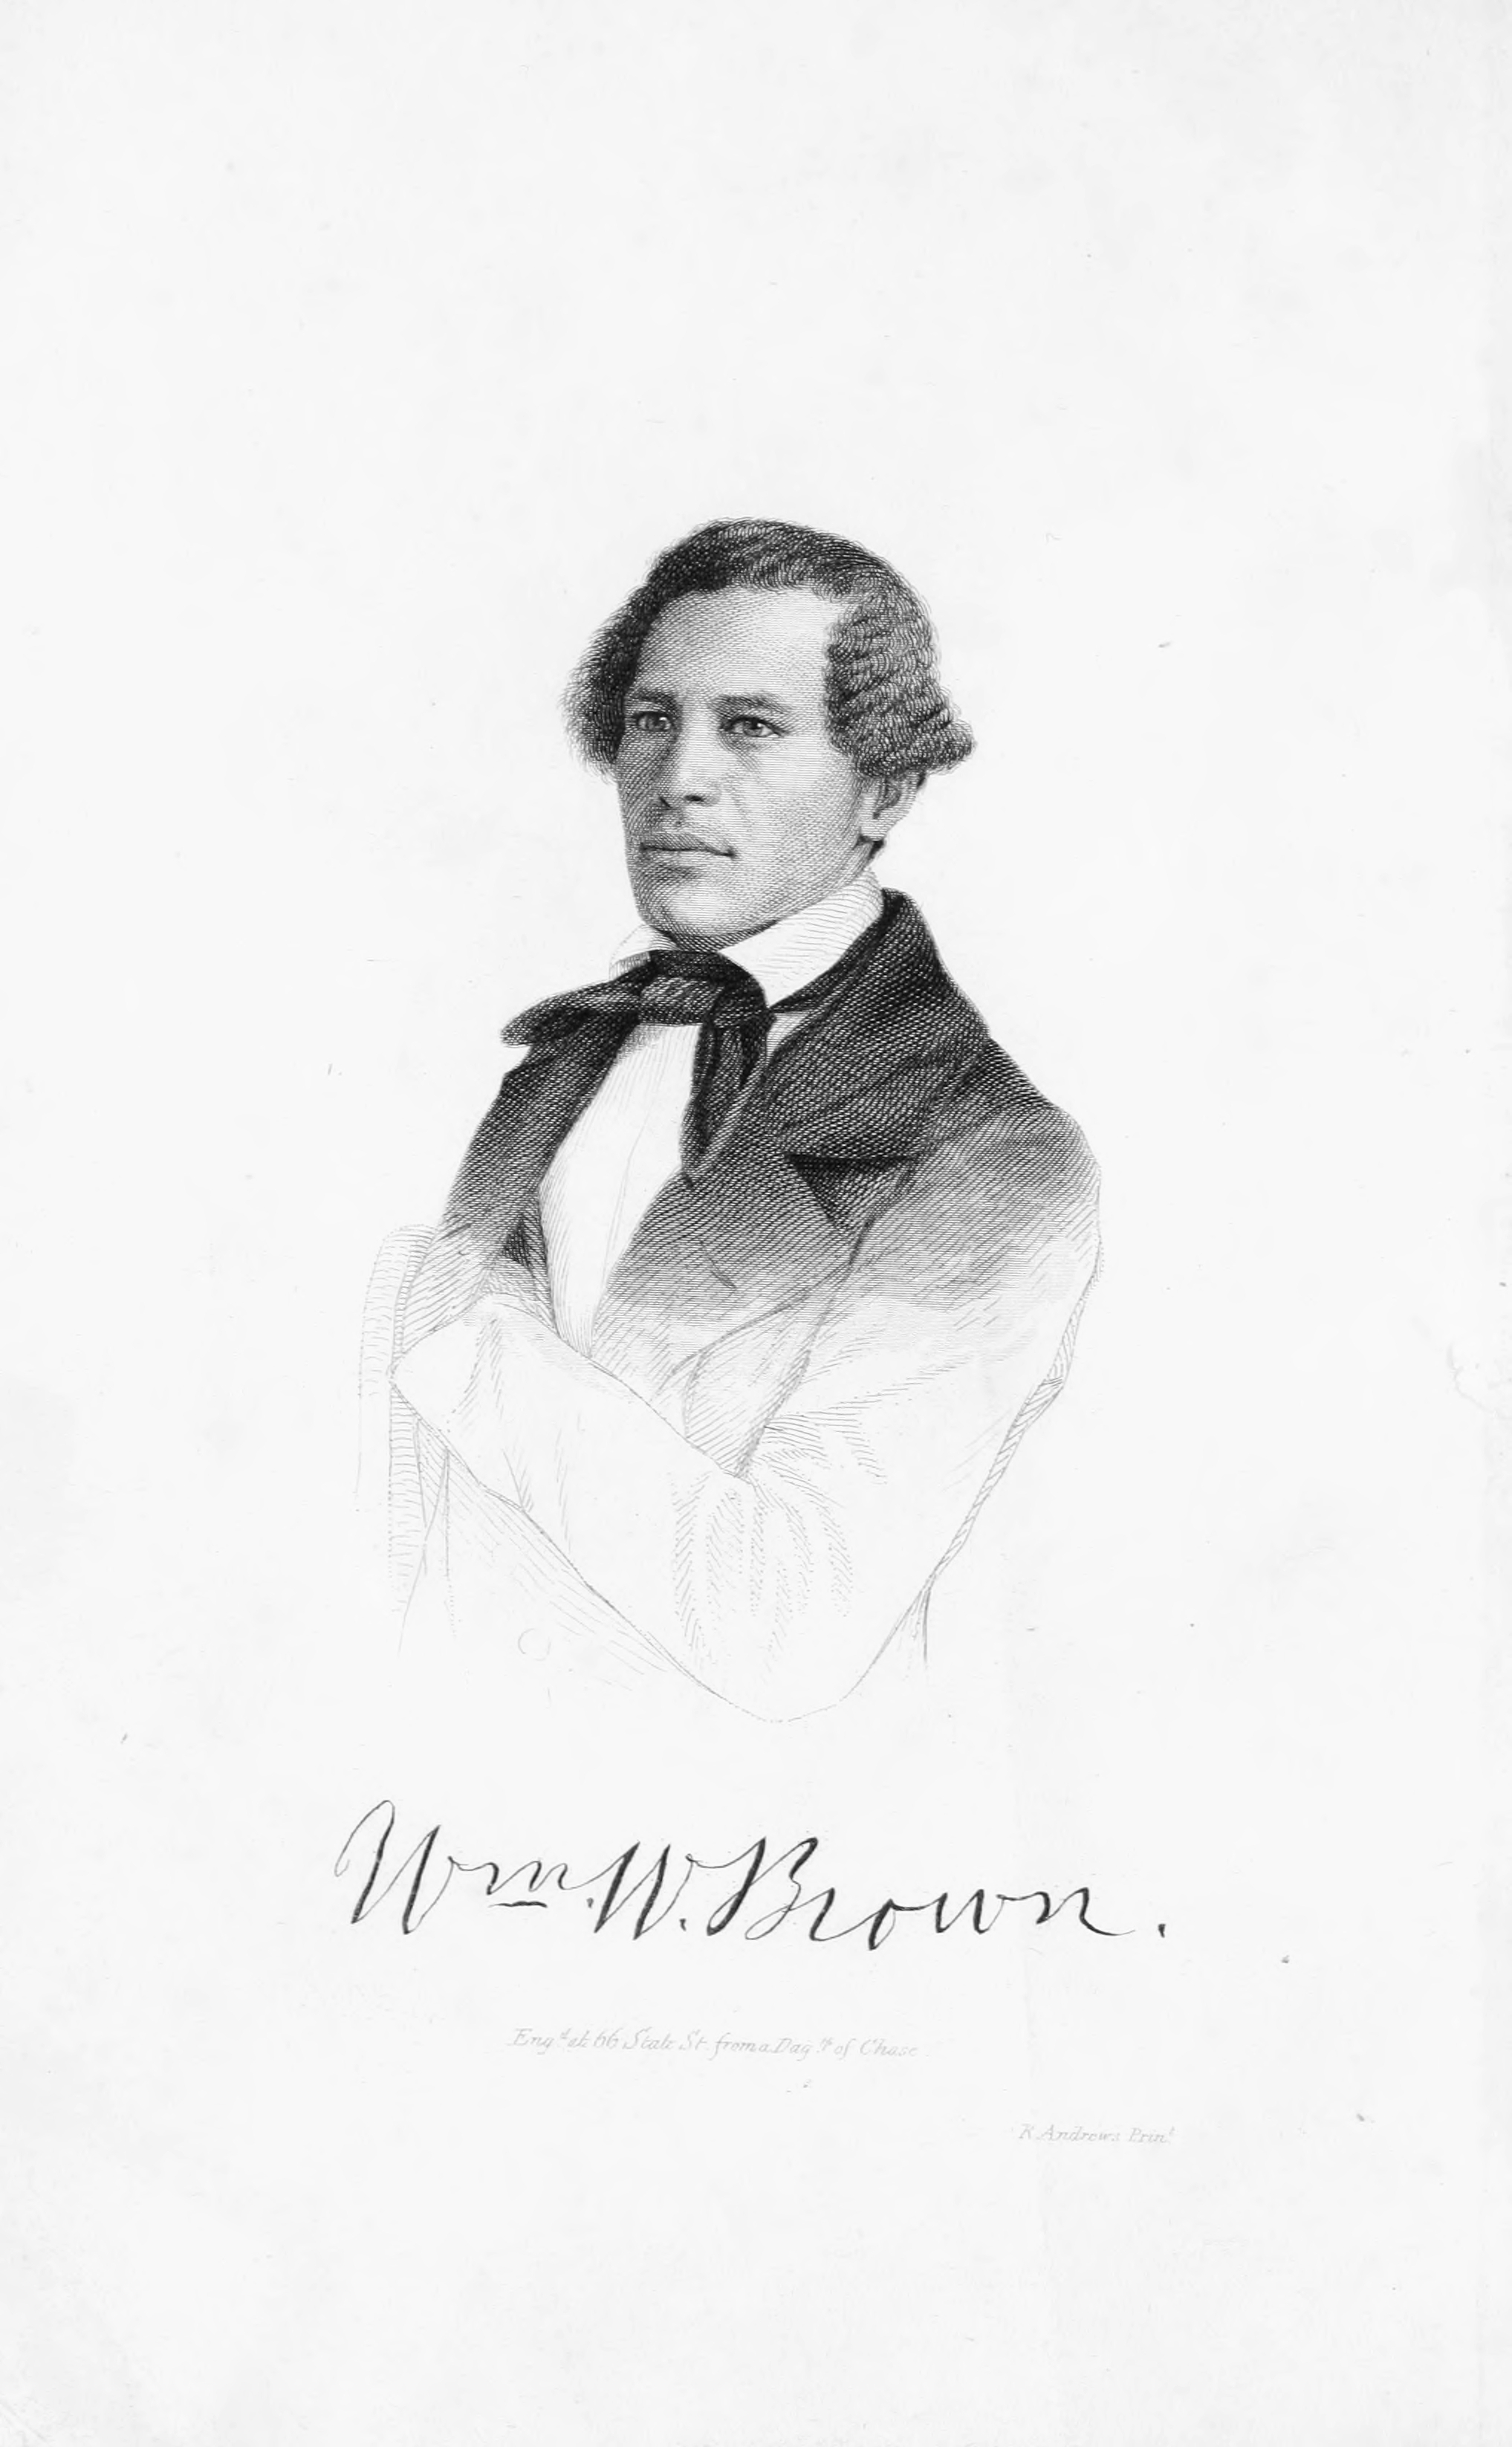
\includegraphics[width=134mm]{./imgs/front1.jpg}  \label{front}
  %\hfill
\end{adjustwidth}
  \caption{}
\end{figure}
\end{vplace}

\thispagestyle{empty}
\end{absolutelynopagebreak}


\pagebreak

\begin{absolutelynopagebreak}
\begin{vplace}
\begin{figure}[H]
\begin{adjustwidth}{-1.8cm}{}
  %\centering
  \vspace*{-2.6cm}
  %\hspace{-0.5cm}
  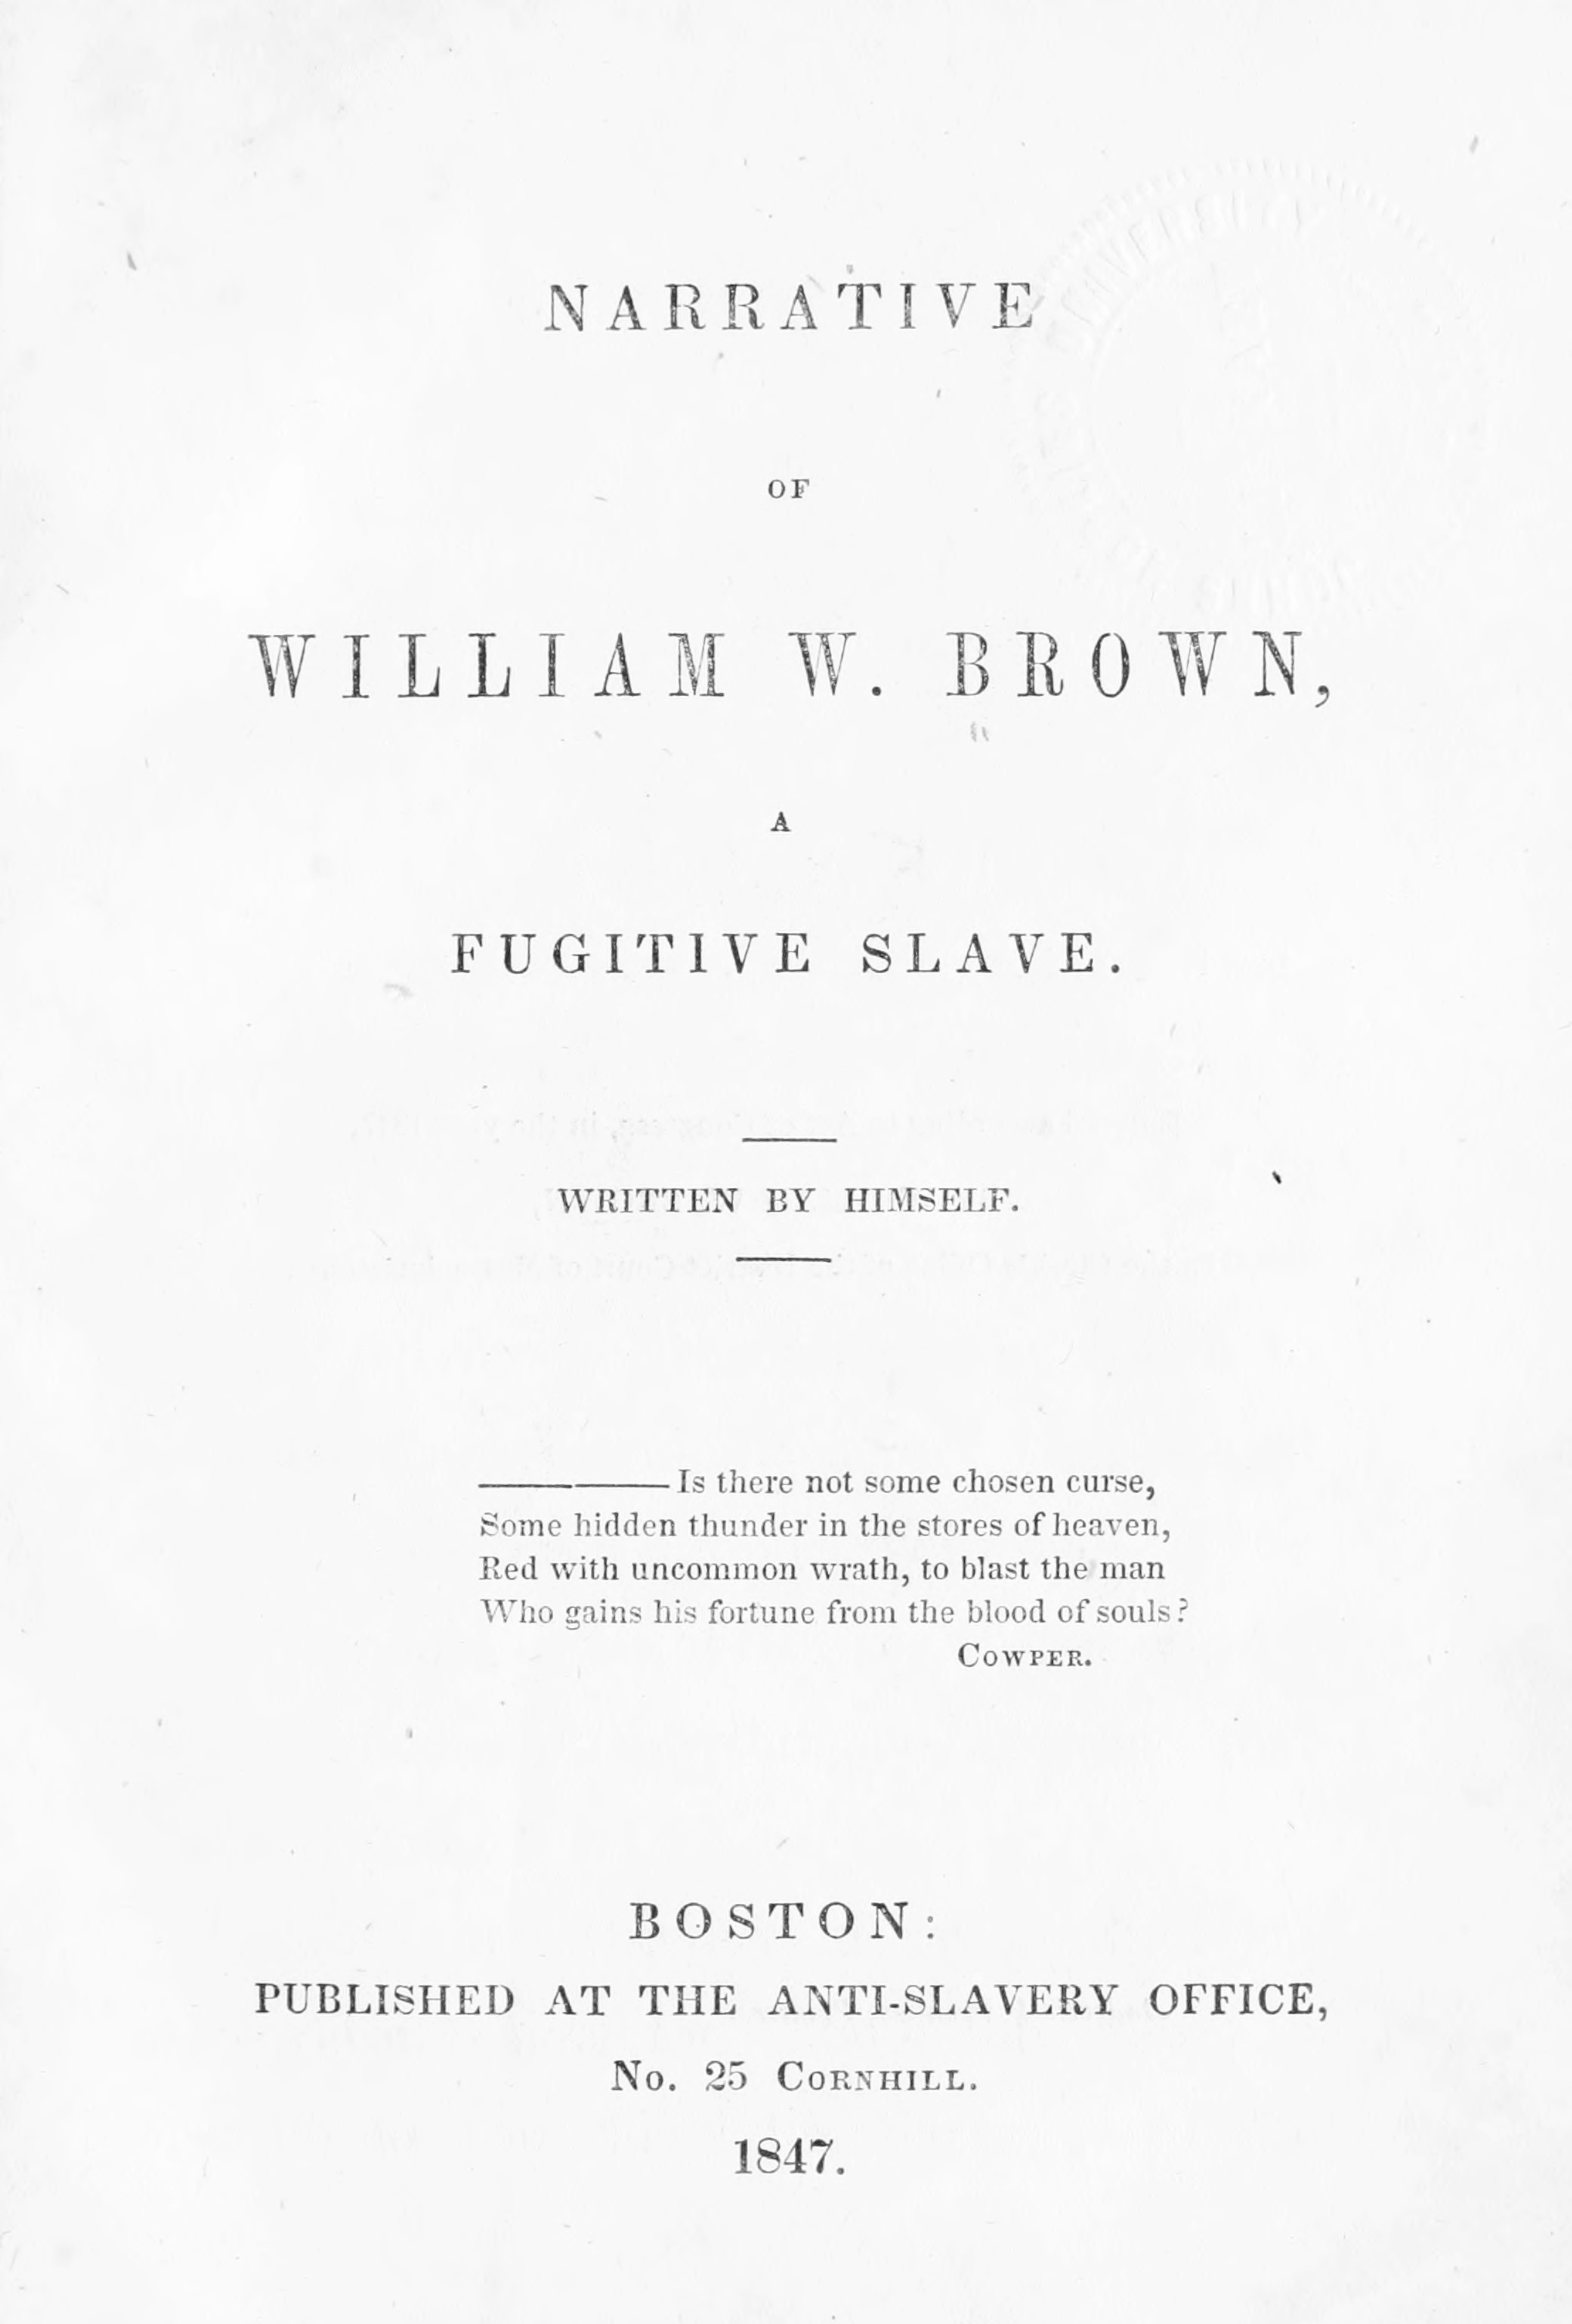
\includegraphics[width=134mm]{./imgs/front2.jpg}  
  %\hfill
\end{adjustwidth}
  \caption{Frontispício da primeira edição da autobiografia de William Wells Brown, publicada em Boston em 1847.}
\end{figure}
\end{vplace}

\thispagestyle{empty}
\end{absolutelynopagebreak}


\movetooddpage
\addcontentsline{toc}{part}{Narrativa de William Wells Brown}
\part*{Narrativa de William Wells Brown, escravo fugitivo, escrita por ele mesmo}


\chapter*{}
\thispagestyle{empty}
\begin{verse}
---Is there not some chosen curse,\\
Some hidden thunder in the stores of heaven,\\
Red with uncommon wrath, to blast the man\\
Who gains his fortune from the blood of \qb{}souls?\footnote{Tradução: ``Não haveria uma maldição seleta/ Um trovão oculto no arsenal celeste,/ Rubro com fúria especial, para fulminar o homem/ Que faz sua fortuna com o sangue das almas?''}
\end{verse}
\begin{flushright}
\versal{COWPER}\footnote{Brown atribui esses versos ao poeta inglês William
  Cowper (1731--1800). Na verdade, a passagem pertence à peça \emph{Cato,
  A Tragedy}, de Joseph Addison (1672--1719).}
\end{flushright}

\chapter{Para Wells Brown, de Ohio}

Treze anos atrás eu batia à sua porta, cansado, fugindo dos grilhões e
da chibata. Era forasteiro e você me hospedou. Estava faminto e você me
deu de comer. Estava nu e você me deu de vestir. A escravidão me negara
até um nome pelo qual pudesse ser chamado entre os homens, e você me deu
o seu. Eu seria uma criatura deveras vil se esquecesse tudo que te devo 
ou fizesse o que fosse para desonrar o seu nome sagrado!

Como pequeno testemunho da gratidão que tenho pelo meu primeiro
benfeitor, tomo a liberdade de lhe dedicar esta pequena \emph{Narrativa} dos
sofrimentos dos quais estava fugindo quando fui agraciado com a sua
compaixão. Entre as multidões que receberam seu auxílio, é bem possível
que você não se lembre de mim; mas até que eu esqueça Deus e a mim
mesmo, nunca me esquecerei de você.

Teu amigo agradecido

\begin{flushright}
\emph{William Wells Brown}
\end{flushright}

\chapter{Carta de Edmund Quincy} %, esq.

\begin{flushright}
\emph{Dedham, 1º de julho de 1847}
\end{flushright}

\begin{flushleft}
Para William Wells Brown
\end{flushleft}

Meu caro amigo: Agradeço sinceramente pelo privilégio de ler o
manuscrito da sua \emph{Narrativa}. Li"-a com profundo interesse e fiquei
emocionado. Tenho certeza que será, além de um enorme sucesso, de
extrema utilidade. Ela apresenta uma fase diferente do sistema
escravista infernal em relação àquela retratada na história admirável do
Sr.\,Douglass\footnote{Frederick Douglass (1819--1895): Abolicionista,
  jornalista e político americano. Sua primeira autobiografia, a
  \emph{Narrativa da vida de Frederick Douglass, um escravo americano},
  foi um sucesso de vendas na época e ainda é considerada um clássico da
  literatura dos \versal{EUA}.} e nos permite vislumbrar as crueldades atrozes de
outras partes do seu domínio.

As oportunidades que você teve de observar o funcionamento desse sistema
maldito foram particularmente grandes. Suas experiências na Lavoura, na
Casa Grande e, especialmente, no Rio, a serviço de Walker, o traficante
de escravos, quase não encontra paralelo entre outros indivíduos, e
certamente nenhum que tenha demonstrado a competência para descrevê"-los.
O que admiro, e o que me assombra, na sua \emph{Narrativa} é a calma e a
simplicidade com que descreve cenas e ações que poderiam muito bem
``levar as próprias pedras a se erguerem em motim'' contra a Instituição
Nacional que as tornam possíveis.

Como irá perceber, em muito pouco fiz uso da gentil permissão que me deu
para alterar aquilo que escreveras. Corrigir alguns equívocos, que \label{ref1}
pareciam ser meros erros de cópia, cometidos na pressa da composição,
empreendida em condições desfavoráveis, e sugerir alguns abreviamentos,
foi tudo que ousei fazer. Seria muita audácia da minha parte, e muita
vaidade também, tentar melhorar as descrições do que você viu e sofreu.
Algumas das cenas fariam jus ao próprio De Foe.

Confio que sua narrativa terá ampla circulação e tenho certeza de que
ela o merece. Deve possuir uma natureza diferente da minha o homem que
encerre a leitura da \emph{Narrativa} sem acreditar que entende a escravidão
melhor do que nunca, e a odeie ainda mais.

Fiel e respeitosamente, 

Seu amigo

\begin{flushright}
\emph{Edmund Quincy}
\end{flushright}

\chapter{Prefácio à primeira edição}

Os amigos da liberdade podem comemorar o surgimento da \emph{Narrativa} a
seguir, que acrescenta mais um volume à crescente literatura
antiescravista contemporânea. Como afirmou um grande observador da
natureza humana: ``Deixem"-me compor as canções de uma nação e não me
importarei com quem compõe suas leis'';\footnote{Frase de Andrew Fletcher
  (1655--1716), escritor e político antiunionista escocês.} e com o
mesmo grau de verdade pode"-se dizer que, entre um povo leitor como o
nosso, nossos livros irão ao menos caracterizar nossas leis. É uma
influência que avança silenciosamente em sua missão, mas jamais deixa de
encontrar o caminho a muitos corações calorosos para acender em seus
altares a chama da liberdade que um dia se conflagrará no incêndio que
há de consumir a opressão.

Este livreto é uma voz emanando da prisão, desvendando os feitos
sombrios que nela são perpetrados. Nossa causa recebe um grande socorro
dessa fonte. Os nomes daqueles que vieram de lá, e que batalharam
valorosamente pela justiça, não precisam ser registrados aqui. As obras
de alguns deles são monumentos eternos à divindade e seu registro
perpétuo encontra espaço nos corações agradecidos dos cativos redimidos.

Poucas pessoas tiveram maior oportunidade para conhecer a escravidão em
todos os seus aspectos mais terríveis do que William W. Brown. Ele
esteve por trás dos panos. Visitou suas câmaras secretas. Os ferros dela
penetraram a sua alma. Os laços mais caros da natureza foram fendidos em
sua pessoa. Uma mãe foi açoitada cruelmente perante seus próprios olhos.
Um pai\ldots{} mas, ah, escravo não tem pai. Um irmão se tornou vítima
de sua própria misericórdia. Uma irmã foi entregue ao controle
irresponsável do pálido opressor. E esta nação assente com a cena. A
União americana sanciona esses feitos. A Constituição protege os
criminosos. A religião americana santifica o crime. Mas a maré está
virando. Uma corrente submarina arrasta o país para a frente. Uma voz de
alerta, de admoestação, de censura, de rogo, está soando. Mãos seguram
mãos e corações se mesclam com corações na grande obra da salvação dos
escravos.

Mesmo agora, as convulsões do monstro evidenciam suas feridas profundas.

O autor desta \emph{Narrativa} foi emprestado pelo seu senhor para um
``\emph{traficante de almas}'' e testemunhou todos os horrores do
tráfico, desde a compra do rebanho humano nos estados criadores de
escravos, que produzem uma cena constante da separação das vítimas dos
seus entes queridos, até a sua venda final no mercado do Sul, para serem
exauridos em sete anos ou entregues à luxúria dos \emph{cristãos}
sulistas.

Muitas cenas pungentes são retratadas explicitamente, mas também com uma
simplicidade e uma engenhosidade que transmitem a certeza sobre a
veracidade da imagem.

Este livro fará muito para desmascarar aqueles que ``se vestiram com o
libré da corte celestial'' a fim de disfarçar a monstruosidade dos seus
atos.

Durante os últimos três anos, o autor dedicou todas as suas energias à
causa antiescravista. Labutando sob todas as deficiências e desvantagens
decorrentes de ter sido educado sob a escravidão, de ter sido sujeitado,
como foi desde nascença, a todos os males e privações inerentes à sua
condição, ainda assim ele seguiu em frente, atraído ao trabalho pelo
amor à liberdade, estimulado pela memória do próprio sofrimento, instado
pela consideração de que mãe, irmãos e irmã ainda agonizavam no
cativeiro ao lado de três milhões de filhos do Nosso Pai, sustentado por
uma fé inabalável na onipotência da verdade e no triunfo final da
justiça, para defender a causa dos escravos, e pela eloquência da sua
sinceridade transmitiu a certeza a muitas mentes e arregimentou a
simpatia e a cooperação de muitos outros em prol da causa.

Seu trabalho se limitou principalmente ao oeste do estado de Nova York,
onde conquistou muitos amigos queridos com seu zelo incansável, sua
energia perseverante, sua fidelidade constante e sua bondade universal.

Leitor, és um abolicionista? O que fizestes pelo escravo? O que fazes
por ele? O que pretendes fazer? Uma grande obra nos espera. Quem há de
ficar parado? Em termos comparativos, este é o grande movimento
humanitário da nossa era, engolindo, por ora, todas as outras questões.
O curso da história humana, obediente às leis imutáveis da nossa
existência, avança rapidamente para uma crise final. Eis a pergunta:

\begin{verse}
Have ye chosen, O my people, on whose \qb{}party ye shall stand,\\
Ere the Doom from its worn sandal shakes \qb{}the dust against our land?\footnote{Tradução: ``Já escolhestes, ó, meu povo, que partido ireis tomar,/ Antes que o Destino de suas sandálias gastas sacuda a poeira contra a
nossa terra?''. Versos de \emph{The Present Crisis}, do poeta
  romântico americano James Russell Lowell (1819--1891). ``Sacudir a
  poeira'' é uma referência a Mateus 10:14 e à antiga prática judaica de
  sacudir a poeira dos pés ao sair de cidades não"-judaicas para indicar
  separação do mundo gentio.}
\end{verse}

Você é cristão? Esta é a realização do Cristianismo prático, e não há
outra forma. O Cristianismo é \emph{prático} em sua própria essência e
natureza. É uma vida que nasce da alma imbuída com o seu espírito. É
amigo da causa missionária? Este é o maior empreendimento missionário de
hoje. Três milhões de \emph{cristãos}, transformados em pagãos pela lei,
anseiam pelas boas novas do Evangelho da liberdade. É amigo da Bíblia?
Vem, então, e nos ajuda a restaurar a vista para esses milhões cujos
olhos foram furados pela escravidão, para que possam enxergar e ler a
Bíblia. Ama Deus, a quem nunca viu? Então manifesta esse amor e devolve
ao irmão que já vistes a sua legítima herança, da qual foi privado por
tanto tempo e com tanta crueldade.

Não é por uma única geração de três milhões que trabalhamos, por mais
sublime que seja tal esforço. É pela humanidade, ao redor do mundo, não só agora, mas por todos os tempos, e por todas as gerações futuras:

\begin{verse}
For he who settles Freedom's principles,\\
Writes the death"-warrant of all tyranny.\footnote{Tradução: ``Pois quem estabelece os princípios da Liberdade/ Redige a sentença de morte
de toda a tirana.'' De \emph{L'Envoi}, poema final de \emph{A
  Year's Life}, o primeiro livro de James Russell Lowell.}
\end{verse}

É um trabalho vasto, um empreendimento glorioso, digno da devoção
inarredável de toda a vida dos grandes e dos bons.

O escravismo e os escravistas devem ser convertidos em seres
ignominiosos e detestáveis. Devem perder sua respeitabilidade e sua
reputação cristã. Devem ser tratados como ``ladrões de homens, culpados
do mais grave roubo e pecadores de primeira ordem''.\footnote{Passagem da
  Disciplina da Igreja Presbiteriana dos \versal{EUA}, adotada em 1794 e
  eliminada em 1816 com a influência crescente dos escravistas na
  Assembleia Geral.} Seus cúmplices mais culpados, na pessoa dos
\emph{apologistas nortistas}, tanto na Igreja quanto no Estado, devem
ser colocados na mesma categoria. Os homens honestos devem ser
convencidos a ver esses crimes com a mesma aversão e desprezo que
destinam aos ladrões e assassinos menos culpados, até que:


\begin{verse}
The common damned shun their society,\\
And look upon themselves as fiends less \qb{}foul.\footnote{Tradução: ``Os condenados comuns rejeitam a sua sociedade/ E se consideram demônios menos atrozes.'' De \emph{The Grave}, do poeta
  escocês Robert Blair (1699--1746).}
\end{verse}

Quando o crime da escravidão receber sua justa sentença, o trabalho
estará completo. E terá chegado o dia glorioso:

\begin{verse}
When man nor woman in all our wide \qb{}domain,\\
Shall buy, or sell, or hold, or be a slave.\footnote{Tradução: ``Quando nem homem nem mulher em nossos vastos domínios/ Há de comprar, ou vender, ou ter, ou ser escravo.'' Paráfrase dos versos finais de \emph{Inscription under the Picture of an Aged Negro"-woman}, do poeta escocês James Montgomery (1771--1854).}
\end{verse}

\bigskip

\begin{flushright}
\emph{J. C. Hathaway}

Farmington, Nova York, 1847.
\end{flushright}



\chapter*{Capítulo I}
\addcontentsline{toc}{chapter}{Capítulo \textsc{i}}

Nasci em Lexington, Kentucky. O homem que me roubou assim que nasci \label{ref5}
registrava o nascimento de todos os bebês que alegava serem de sua
propriedade em um livro que mantinha para esse fim. O nome de minha mãe
era Elizabeth. Ela teve sete filhos, a saber: Solomon, Leander,
Benjamin, Joseph, Millford, Elizabeth e eu. Nenhum de nós tinha o mesmo
pai que o outro. O nome de meu pai, como soube de minha mãe, era George
Higgins. Ele era um homem branco, aparentado com meu senhor, e ligado a
algumas das famílias mais proeminentes do Kentucky.

Meu senhor possuía cerca de quarenta escravos, vinte e cinco dos quais
eram lavradores. Ele se mudou do Kentucky para o Missouri quando eu era
ainda muito jovem e se estabeleceu cinquenta ou setenta quilômetros
acima de St.\,Charles, no Rio Missouri, onde, além da clínica de
medicina, praticava a moagem de cereais, o comércio e a agricultura. Ele
tinha uma fazenda grande, e seus principais produtos eram o tabaco e o
cânhamo. As senzalas ficavam situadas nos fundos da fazenda, com a casa
do feitor, chamado Grove Cook, em seu meio. Ele era encarregado de toda
a fazenda e, por não ter família, mantinha uma mulher que cuidava da
casa para ele; era ela a responsável por distribuir as provisões para os
lavradores.

Também havia uma mulher que ficava nos alojamentos para cozinhar para os
trabalhadores do eito, que eram convocados para a sua labuta incessante
todos os dias às quatro da manhã. O sino pendurado em um poste junto à
casa do feitor repicava e então eles tinham meia hora para fazer seu
desjejum e partir para o campo. Às quatro e meia, o feitor soava um
berrante, sinalizando o começo do trabalho, e todos que não estivessem
presentes naquele instante recebiam dez chibatadas do chicote com o qual
o feitor estava sempre armado. O cabo tinha quase um metro de
comprimento, com a ponta cheia de chumbo, e a chibata de couro tinha
dois metros, com arame trançado na ponta. O chicote era aplicado com
bastante frequência e liberdade, e qualquer pequeno delito por parte de
um escravo era causa para a sua utilização. Durante a época em que o Sr.\,Cook foi feitor, eu era criado doméstico, uma situação preferível à do
escravo do eito, pois eu era mais bem alimentado, me vestia melhor e não
era forçado a me levantar com o tocar do sino, e sim cerca de meia hora
depois. Muitas vezes fiquei deitado, escutando os estalos da chibata e
os berros dos escravos. Minha mãe trabalhava no eito e, uma manhã,
chegou ao campo dez ou quinze minutos depois dos outros. Logo que chegou
no local onde eles iriam trabalhar, o feitor começou a açoitá"-la.

--- Ah! por favor\ldots{} Ah! por favor\ldots{} Ah! por favor --- ela
gritava.

Essas eram as palavras recorrentes dos escravos, implorando por piedade
das mãos dos seus opressores. Eu reconheci a voz dela, saltei do meu
catre e saí correndo para a porta. A lavoura ficava longe da casa, mas
ainda assim eu escutava cada estalo do chicote, cada grito e gemido da
minha pobre mãe. Permaneci junto à porta, sem ousar ir além. Senti um
calafrio correr de cima a baixo e caí em prantos. Após a décima
chibatada, o som do chicote cessou e eu voltei para a cama, consolado
apenas pelas lágrimas. O sol ainda não havia nascido.

\chapter*{Capítulo II}
\addcontentsline{toc}{chapter}{Capítulo \textsc{ii}}

Meu senhor era um demagogo político e logo encontrou quem estivesse
disposto a obter"-lhe um cargo em troca dos favores que poderia prestar,
e poucos anos após sua chegada ao Missouri ele foi eleito para o
Legislativo estadual. Enquanto ele estava ausente, o Sr.\,Cook, o feitor,
ficava encarregado de tudo, e logo se tornou ainda mais tirânico e
cruel. Entre os escravos da fazenda havia um que atendia pelo nome de
Randall. Era um homem de cerca de um metro e oitenta de altura, esbelto,
conhecido por todos por sua enorme força, e considerado o escravo mais
valioso e capaz de toda a plantação; contudo, por melhor ou mais útil
que seja um escravo, ele quase nunca escapa da chibata. Mas Randall era
uma exceção. Ele estava na fazenda desde que eu me lembrava, mas eu
nunca o vira ser castigado. Isso não era graças ao senhor ou ao feitor.
Muitas vezes eu o ouvi declarar que nenhum branco jamais o açoitaria,
que morreria antes disso.

Desde o dia em que chegara à fazenda, Cook sempre declarara que podia e
iria castigar qualquer crioulo que trabalhasse sob o seu comando no
campo. Meu senhor lhe dissera inúmeras vezes que não tentasse açoitar
Randall, mas o feitor estava decidido. Assim que se tornou o único
ditador da fazenda, determinou que chegara o momento de executar suas
ameaças. Um dia, ordenou uma tarefa muito difícil, mais do que Randall
seria capaz de fazer; e à noite, como a tarefa não estava concluída,
disse a Randall que deveria lembrar dele na manhã seguinte. No outro
dia, depois que os escravos haviam feito seu desjejum, Cook chamou
Randall e disse que pretendia açoitá"-lo. O feitor ordenou que ele
cruzasse as mãos e fosse amarrado. Randall perguntou por que queria
açoitá"-lo. A resposta foi que ele não completara a tarefa do dia
anterior. Randall disse que a tarefa era grande demais, e que a teria
realizado se não fosse por isso. Cook respondeu que não fazia diferença,
que era preciso açoitá"-lo. Randall ficou em silêncio por um instante e
então respondeu:

--- Sr.\,Cook, eu sempre tentei agradá"-lo desde que o senhor chegou à
fazenda, mas o senhor está decidido a não se satisfazer com o meu
trabalho. Deixe"-me trabalhar como posso. Homem nenhum colocou as mãos em
mim para me açoitar nos últimos dez anos, e há muito concluí que não
existe homem vivo que vá me açoitar.

Cook, percebendo pelo olhar e os gestos decididos de Randall que este
iria resistir, chamou três escravos que estavam trabalhando, ordenou
que agarrassem Randall e o amarrassem. Os escravos ficaram parados; eles
conheciam Randall, e sabiam muito bem a força deste, então tinham medo
de atacá"-lo. Logo que Cook ordenou que os homens o agarrassem, Randall
se virou para eles e disse:

--- Rapazes, vocês todos me conhecem, sabem que posso com qualquer de
vocês três e que o homem que encostar em mim há de morrer. Esse branco
não consegue me castigar sozinho, então chamou vocês para ajudá"-lo.

O feitor não conseguiu convencê"-los a amarrar Randall e finalmente
ordenou que todos voltassem para o trabalho.

Randall não ouviu nada do feitor por mais de uma semana. Uma manhã, no
entanto, enquanto os escravos estavam no eito, ele chegou com três
amigos, Thompson, Woodbridge e Jones. Eles foram até onde Randall estava
trabalhando e Cook ordenou que deixasse o trabalho de lado e os
acompanhasse até o celeiro. Randall se recusou, então foi atacado pelo
feitor e seus companheiros; ele reagiu e os derrotou um a um,
prostrando"-os no chão. Woodbridge sacou sua pistola e disparou,
derrubando"-o com uma bala. Os outros saltaram sobre ele, desferindo
porretadas sobre a cabeça e no rosto até que conseguiram amarrá"-lo.
Depois, Randall foi levado ao celeiro e amarrado a uma trave. Cook lhe
deu mais de cem chibatadas com um chicote de couro pesado, mandou lavar
as feridas com salmoura e deixou"-o amarrado durante o dia. No dia
seguinte, ele foi desamarrado e levado à ferraria, onde uma bola com
corrente foi presa à sua perna. Randall foi forçado a trabalhar no campo
e completar a mesma quantidade de trabalho que todos os outros. Quando
voltou para casa, seu senhor ficou muito contente em descobrir que
Randall fora domado na sua ausência.

\chapter*{Capítulo III}
\addcontentsline{toc}{chapter}{Capítulo \textsc{iii}}

Pouco depois, meu senhor se mudou para a cidade de St.\,Louis e comprou
uma fazenda a seis quilômetros de distância, que colocou sob a
supervisão de um feitor chamado Friend Haskell, um típico yankee da Nova
Inglaterra. Os yankees são famosos por darem os feitores mais cruéis de
todos.

Minha mãe foi alugada na cidade, e eu também fui alugado lá pelo Major
Freeland, que mantinha uma taverna. Oriundo da Virgínia, ele estava
envolvido com corridas de cavalo, rinhas de galos e jogos de azar e era
um bêbado inveterado. Havia dez ou doze criados na casa e, quando ele
estava presente, o lugar era uma balbúrdia e um pandemônio. Em seus
acessos de fúria, ele atirava cadeiras nos criados; em seus momentos
mais racionais, quando desejava castigar alguém, os amarrava e açoitava
no defumadouro, então acendia uma fogueira com talos de tabaco para
defumá"-los. Isso que ele chamava de uma ``\emph{virginiada}''.

Reclamei para o meu senhor do tratamento que recebia do Major Freeland,
mas não fez diferença. Ele não dava nenhuma importância a isso, desde
que recebesse o dinheiro pelo meu trabalho. Após morar com o Major \enlargethispage{\baselineskip}
Freeland por cinco ou seis meses, fugi e me escondi na floresta perto da
cidade. Quando a noite caiu, me dirigi à fazenda do meu senhor, mas tive
medo de ser avistado, sabendo que se o feitor, o Sr.\,Haskell, me
achasse, eu seria arrastado de volta para o Major Freeland; assim,
permaneci na floresta. Um dia, enquanto estava na floresta, ouvi cães
ladrando e uivando, e logo eles se aproximaram tanto que reconheci os
sabujos do Major Benjamin O'Fallon, que criava cinco ou seis cães para
caçar escravos fugitivos.

Logo que me convenci de que eram eles, soube que a fuga seria
impossível. Encontrei refúgio na copa de uma árvore e os cães logo a
cercaram, e ali permaneceram até os caçadores chegarem, meia hora ou
três quartos de hora depois. Dois homens acompanhavam os cães e, assim
que chegaram, me mandaram descer. Eu desci e fui amarrado e levado à
cadeia de St.\,Louis. O Major Freeland logo apareceu, me soltou e ordenou
que eu o seguisse, o que fiz. Após voltarmos para casa, ele me amarrou
no defumadouro e eu fui açoitado horrivelmente. Após o Major me castigar
até se dar por satisfeito, ele mandou chamar Robert, seu filho, um jovem
de dezoito ou vinte anos, para garantir que eu fosse defumado. Ele
acendeu uma fogueira com talos de tabaco que logo me deixou tossindo e
espirrando. Esse era o modo como seu pai lidava com seus escravos na
Virgínia, Robert me contou. Após aplicarem o que consideravam uma
defumada decente, fui desamarrado e colocado no trabalho mais uma vez.

Robert Freeland era ``filho de peixe''. Apesar de muito jovem,
frequentemente chegava em casa embriagado. Creio que hoje ele é o
comandante popular de um barco a vapor no rio Mississippi. Os negócios
do Major Freeland logo decaíram e eu fui colocado a bordo do vapor
\emph{Missouri}, que fazia a rota entre St.\,Louis e Galena. O comandante
do navio era William B. Culver. Permaneci a bordo durante a temporada de
navegação, a época mais agradável que havia vivenciado até então. Ao
final do período, fui alugado pelo Sr.\,John Colburn, que mantinha o
Missouri Hotel. Ele era oriundo de um dos Estados Livres, mas não acho
que jamais pôs os pés nesta terra de Deus um inimigo mais inveterado dos
negros. Na época, o hotel era um dos maiores da cidade e empregava vinte
ou trinta criados, quase todos escravos.

O Sr.\,Colburn era muito perverso, e não apenas com os criados, mas com a
esposa também, uma excelente mulher e uma pessoa da qual nunca observei
um criado receber uma única palavra de rispidez, assim como nunca
observei uma palavra de gentileza do marido. Entre os escravos
empregados no hotel havia um chamado Aaron, que pertencia ao Sr.\,John F.
Darby, um advogado. Aaron lavava as facas. Um dia, uma das facas foi
colocada à mesa menos limpa do que poderia estar. Por essa ofensa, o Sr.\,Colburn atou Aaron no depósito de lenha e lhe deu cinquenta chibatadas
nas costas nuas com um chicote de couro, e depois me fez lavar Aaron com
rum. Isso pareceu deixá"-lo em mais agonia do que as vergastadas. Depois
que foi desamarrado, ele voltou para a casa do seu senhor e reclamou do
tratamento que recebera. O Sr.\,Darby também não deu nenhuma atenção ao
que ele tinha a dizer e o mandou de volta na mesma hora. Colburn, ao
descobrir que Aaron fora reclamar para o seu senhor, o amarrou de novo e
o castigou pior do que antes. As costas do pobre rapaz foram
literalmente cortadas em pedacinhos, tanto que não teve como trabalhar
pelos próximos dez ou doze dias.

Entre os criados havia também uma menina de nome Patsey cujo senhor
morava no campo. Uma noite, o Sr.\,Colburn a amarrou e açoitou até que
vários dos hóspedes apareceram para implorar que ele parasse. O motivo
para o castigo era o seguinte. Ela estava noiva de um homem que
pertencia ao Major William Christy, que residia seis ou sete quilômetros
ao norte da cidade. O Sr.\,Colburn a proibira de ver John Christy.
Supostamente, o motivo era o apreço que ele mesmo tinha por Patsey. Ela
foi encontrá"-lo naquela tarde e John voltou para casa com ela. O Sr.\,Colburn pretendia castigar John se ele passasse pelo cercado, mas este
conhecia muito bem o temperamento do rival e se manteve a uma distância
segura. Assim, ele extraiu sua vingança da pobrezinha. Se todos os
capatazes do mundo fossem reunidos, não creio que se encontraria entre
eles um homem mais cruel do que John Colburn, e este um nortista ainda
por cima.

Enquanto eu morava no Missouri Hotel, ocorreu uma circunstância que me
causou enorme infelicidade. Meu senhor vendeu minha mãe e todos os seus
filhos, exceto por mim. Foram todos vendidos para pessoas diferentes na  
cidade de St.\,Louis.

\chapter*{Capítulo IV}
\addcontentsline{toc}{chapter}{Capítulo \textsc{iv}}

Logo fui retirado das mãos do Sr.\,Colburn e alugado para Elijah P.
Lovejoy, na época editor e proprietário do \emph{St.\,Louis Times}. Nesse
período, meu trabalho era principalmente na tipografia, atendendo os
trabalhadores, manejando a prensa etc. O Sr.\,Lovejoy era um homem muito
bom, absolutamente o melhor senhor que jamais tive. A ele mais do que
ninguém, e ao meu emprego na tipografia, devo o pouco aprendizado que
obtive na escravidão.

Apesar de haver quem considerasse que a escravidão era leve no Missouri,
em comparação com os estados onde se cultiva algodão, açúcar e arroz,
não há parte do nosso país escravista mais famoso pelo barbarismo dos
seus habitantes do que St.\,Louis. Foi aqui que o Coronel Harney, oficial
dos Estados Unidos, açoitou uma escrava até a morte. Foi aqui que
Francis McIntosh, um negro livre de Pittsburgh, foi arrancado do vapor
\emph{Flora} e queimado na fogueira. Durante meus oito anos de
residência na cidade, pude observar pessoalmente inúmeros casos de
extrema crueldade; registrar todos eles ocuparia mais espaço do que
jamais seria possível neste pequeno volume. Assim, apresentarei apenas
mais alguns, além daqueles que já relatei.

O Capitão J. B. Brunt, que residia próximo ao meu senhor, tinha um
escravo chamado John. Este era seu criado pessoal, cocheiro etc. Em uma
ocasião, enquanto guiava seu senhor pela cidade, estando as ruas muito
lamacentas e os cavalos galopando à velocidade, um pouco de lama
respingou em um cavalheiro chamado Robert More. More estava decidido a
se vingar. Três ou quatro meses após o ocorrido, ele comprou John com o
objetivo expresso, disse ele, de ``domar esse mal***o crioulo''. Após a
compra, ele o levou a um ferreiro, prendeu bola e corrente à sua perna e
o colocou a guiar uma parelha de bois. John ficou preso no trabalho
árduo até o ferro ao redor da sua perna desgastar tanto a carne que a
mortificação parecia garantida. Além disso, John me contou que seu
senhor o açoitou regularmente três vezes por semana pelos dois primeiros
meses, e tudo isso para ``domá"-lo''. Seria impossível encontrar em toda
St.\,Louis um homem de aspecto mais nobre do que John antes de cair nas
mãos de More; e uma criatura mais degradada e de espírito mais subjugado
não se encontraria em qualquer fazenda sulista após ele ter sido
sujeitado a esse processo de ``domação'' por três meses. Na última vez
que o vi, ele havia perdido quase completamente o uso dos membros.

Enquanto morava com o Sr.\,Lovejoy, eu frequentemente era mandado aos
escritórios do \emph{Missouri Republican}, publicado pelo Sr.\,Edward
Charles, para fazer pequenas tarefas. Uma vez, enquanto voltava para o
escritório carregando tipos, fui acossado por vários meninos maiores,
filhos de escravistas, que me atacaram com bolas de neve. Por estar
carregando os tipos pesados nas mãos, eu não podia correr deles, então
coloquei os tipos no chão e reagi. Eles se reuniram ao meu redor,
atirando pedras e pedaços de pau até me dominarem, e teriam me capturado
se eu não tivesse saído em disparada. Com a minha retirada, eles se
apossaram dos tipos, e eu não conseguia imaginar como recuperá"-los.
Sabendo que o Sr.\,Lovejoy era um homem muito benevolente, voltei para o
escritório e expliquei para ele toda a situação. Ele me mandou
permanecer onde estava, recrutou um dos aprendizes e foi atrás dos
tipos. Ele logo retornou com o material, mas na volta me informou que
Samuel McKinney lhe dissera que pretendia me açoitar, pois eu havia
machucado seu filho. Logo depois, um dos tipógrafos avistou McKinney se
dirigindo ao escritório e me avisou, permitindo que eu fugisse pela
porta dos fundos.

Como eu não estava lá quando chegou no escritório, McKinney saiu
enfurecido, jurando que me açoitaria até a morte. Alguns dias depois,
enquanto eu caminhava pela Rua Principal, ele me agarrou pela gola e me
deu cinco ou seis bengaladas violentas na cabeça, fazendo com que o
sangue jorrasse do meu nariz e das minhas orelhas de tal forma que
minhas roupas ficaram completamente saturadas de sangue. Após me
espancar o quanto quis, ele me soltou. Eu voltei para o escritório tão
enfraquecido com a perda de sangue que o Sr.\,Lovejoy me mandou para
casa, de volta para o meu senhor. Cinco semanas se passaram antes que eu
voltasse a caminhar. Durante esse período, foi necessário que alguém me
substituísse no escritório, então perdi meu emprego.

Depois que me recuperei, fui alugado pelo Capitão Otis Reynolds como
camareiro de bordo do vapor \emph{Enterprize}, de propriedade dos
senhores John e Edward Walsh, agentes comerciais de St.\,Louis. Na época,
o navio trafegava no Alto Mississippi. Minha função a bordo era atender
cavalheiros e, como o capitão era um bom homem, a posição me agradava;
mas ao estar sempre de um lugar para outro, vendo rostos novos todos os
dias, e sabendo que eles podiam ir aonde bem entendessem, logo fiquei
infeliz. Várias vezes, pensei em desembarcar em algum lugar e tentar uma
fuga para o Canadá, onde sempre ouvira falar que os escravos podiam
viver, ser livres e ficar protegidos.

Mas sempre que essas ideias me ocorriam, minha determinação logo era
abalada pela memória de minha cara mãe, ainda escrava em St.\,Louis, e eu
não suportava a ideia de deixá"-la naquela situação. Tantas vezes ela me
sentara no joelho e contara como me carregara nas costas quando eu era
bebê enquanto trabalhava no eito, chegando a ser frequentemente
castigada por deixar o trabalho para me amamentar, como eu parecia feliz
quando ela me pegava no colo. Quando lembrava disso, decidia nunca
abandonar a terra da escravidão sem minha mãe. Eu pensava que deixá"-la
na escravidão, após tudo o que ela passara e sofrera por mim, seria
renegar tudo o que devia a ela. Além disso, eu tinha três irmãos e uma
irmã na cidade (dois dos meus irmãos haviam morrido).

Minha mãe, meus irmãos Joseph e Millford e minha irmã Elizabeth
pertenciam ao Sr.\,Isaac Mansfield, oriundo de um dos Estados Livres
(Massachusetts, creio). Funileiro por profissão, ele comandava uma
grande manufatura. De todos os meus parentes, minha mãe era a primeira,
minha irmã a segunda. Uma tarde, enquanto as visitava, fiz alguma alusão
à minha proposta de viajar para o Canadá. Minha irmã se sentou ao meu
lado, tomou minhas mãos nas suas e, com os olhos cheios de lágrimas,
disse:

--- Meu irmão, você não vai abandonar mamãe aqui, e sua querida irmã
também, sem um amigo sequer no mundo, vai?

Eu olhei no seu rosto banhado em lágrimas e caí em prantos também.

--- Não, eu nunca hei de desertar você e mamãe.

Ela apertou minhas mãos e disse:

--- Meu irmão, você sempre declara que não vai terminar seus dias na
escravidão. Não consigo imaginar nenhum jeito possível de escapar
conosco; e agora, irmão, você está em um barco a vapor, onde tem alguma chance
de fugir para a terra da liberdade. Por favor, não se prenda por nós. Se
não pudermos obter a nossa liberdade, não queremos ser nós o motivo para
impedi"-lo de conquistar a sua.

Eu não conseguia mais conter meus sentimentos, e quando os extravasei
ela deixou de tocar no assunto. Contrário aos desejos delas, jurei para
mim mesmo que não as deixaria nas mãos do opressor. Parti de volta para
o navio e deitei no meu catre, mas ``o sono fugiu dos meus olhos e o
repouso das minhas pálpebras''.

Algumas semanas depois, na nossa passagem para o Sul, uma turma de
escravos embarcou em Hannibal, com destino ao mercado em Nova Orleans. A
turma era composta por cinquenta ou sessenta homens e mulheres de dezoito a 
quarenta anos. Uma turma de escravos em um navio a vapor sulista, indo
em direção às regiões do algodão e do açúcar, é uma ocorrência tão comum
que ninguém, nem mesmo os passageiros, parecia notar, apesar das
correntes retinirem com cada passo que davam. Contudo, havia um membro
dessa turma que chamava a atenção dos passageiros e da tripulação. Era
uma linda menina, aparentando vinte anos de idade, perfeitamente branca,
com cabelo claro e liso e olhos azuis. Mas não era a brancura da sua
pele que causava sensação em quem a avistava, era sua beleza
praticamente ímpar. A bordo, não demorou para que atraísse os olhos de
todos os passageiros, incluindo as damas, e que o assunto de todas as
conversas fosse a linda escrava. Ela não estava acorrentada. O homem que
reclamava para si esse artigo de mercadoria humana era um tal Sr.\,Walker, um famoso traficante de escravos que residia em St.\,Louis. Entre
passageiros e tripulação, havia uma ânsia geral pela história da menina.
Seu senhor a mantinha sempre junto de si, e teria sido considerado
impudente da parte dos passageiros se dirigir a ela, enquanto os
tripulantes ficavam proibidos de conversar com eles o mínimo que fosse.
Quando chegamos a St.\,Louis, os escravos foram transferidos para um
barco com destino a Nova Orleans, então o histórico dessa bela escrava
permaneceu um mistério.

Continuei a bordo durante a temporada, e não raro tínhamos no navio
turmas de escravo a caminho das fazendas de algodão, açúcar e arroz do
Sul.

Na segunda metade do verão, o Capitão Reynolds deixou o barco e eu fui
mandado para casa. A seguir, fui mandado para trabalhar na fazenda sob o
Sr.\,Haskell, o feitor. Como eu estava longe do campo havia algum tempo,
e desacostumado a trabalhar sob o sol escaldante, foi muito difícil, mas
fui forçado a acompanhar o ritmo dos melhores escravos.

Descobri que havia uma enorme diferença entre o trabalho na cabine de um
navio a vapor e o trabalho em um milharal.

Meu senhor, que estava morando na cidade, logo se mudou para a fazenda,
então eu fui retirado do campo e levado para trabalhar de atendente na
casa grande. Sua esposa era rabugenta e difícil de agradar, mas eu muito
preferia estar sob o seu controle do que do feitor. Eles levaram consigo
o Sr.\,Sloane, um ministro presbiteriano; a Srta.\,Martha Tulley, sua
sobrinha do Kentucky; e William, seu sobrinho. O último frequentava a
família havia vários anos, mas os outros eram recém"-chegados.

O Sr.\,Sloane era um ministro jovem, estava no Sul havia muito pouco
tempo e parecia que todo o seu objetivo de vida era agradar os
escravistas, especialmente meu senhor e minha senhora. Ele pretendia
visitá"-los durante o inverno e não só tentou agradá"-los, creio que foi
admiravelmente bem"-sucedido. Quando eles queriam música, ele cantava;
quando queriam orações, rezava; quando queriam uma história, contava. Em
vez de ensinar teologia ao meu senhor, meu senhor ensinou teologia a
ele. Enquanto estava com o Capitão Reynolds, meu senhor havia
``descoberto a religião'', então havia novas leis na fazenda. Antes, aos
domingos, tínhamos o privilégio de caçar, pescar, fabricar vassouras e
cestos etc., mas tudo isso parou. Agora, todos os domingos éramos
forçados a participar de cultos. Nosso senhor era tão religioso que
convenceu outros a se juntar a ele para contratar um pastor a fim de
pregar para os escravos.

\chapter*{Capítulo V}
\addcontentsline{toc}{chapter}{Capítulo \textsc{v}}

Meu senhor fazia a família orar de manhã e à noite. À noite, os escravos
eram chamados para participar; pelas manhãs, no entanto, eles precisavam
estar no trabalho, então o senhor cuidava de todas as orações. Meu
senhor e minha senhora eram grandes entusiastas do \emph{mint
julep},\footnote{Coquetel tradicional do sul dos \versal{EUA} à base de bourbon,
  hortelã, xarope e gelo triturado.} e todas as manhãs se preparava uma
jarra cheia, da qual eles bebiam livremente, incluindo o jovem William.
Depois que todos bebiam com gosto, eles faziam as orações da família e
então o desjejum. Não posso negar que amava o \emph{julep} tanto quanto
eles, e durante as orações sempre tomava cuidado para me sentar perto da
mesa onde a jarra ficava para me servir enquanto eles se ocupavam das
suas devoções. Quando eles terminavam de rezar, ninguém estava mais
feliz do que eu. Uma manhã, ocorreu um acidente triste. Enquanto me
servia e ficava de olho na minha velha senhora ao mesmo tempo,
acidentalmente deixei a jarra cair no chão, que se despedaçou toda, e
derramou a bebida. Foi um mau bocado para mim; assim que as orações
terminaram, fui levado e castigado duramente.

A família do meu senhor era constituída por ele, pela esposa e pelo
sobrinho, William More, que fora adotado quando tinha poucas semanas.
Como ele e eu tínhamos o mesmo nome, o meu foi alterado para dar
precedência ao dele, apesar de eu ser dez ou doze anos mais velho. Como
a fazenda ficava a seis quilômetros da cidade, eu precisava guiar a
família até a igreja. Eu sempre odiava a chegada do domingo, pois,
durante o culto, era forçado a ficar junto aos cavalos, sob o sol
escaldante ou então na chuva, dependendo do dia.

Um domingo, enquanto passávamos pela casa de D.\,D.\,Page, um cavalheiro
proprietário de uma grande padaria, eu estava sentado na boleia, que
ficava bastante elevada, quando vi o Sr.\,Page perseguindo um escravo
pelo jardim, estalando um chicote comprido e acertando"-o com cada salto.
O homem logo fugiu do quintal, seguido pelo Sr.\,Page. Eles passaram
correndo por nós e, quando o escravo percebeu que seria alcançado, parou
de repente. Page tropeçou nele e caiu nas pedras da calçada, quebrando
uma das pernas e ficando aleijado pelo resto da vida. O mesmo
cavalheiro, pouco tempo antes, havia amarrado Delphia, uma de suas
mulheres, e a açoitado quase até a morte; contudo, ele era também
diácono da igreja batista e em boa situação com todos. Pobre Delphia! Eu
a conhecia bem e fui chamado para visitá"-la na sua convalescença; nunca
hei de me esquecer do seu estado. Ela pertencia à mesma igreja que o seu
senhor.

Logo depois disso, fui alugado pelo Sr.\,Walker, o mesmo homem que
mencionei que carregava turmas de escravos rio abaixo no vapor
\emph{Enterprize}. Ao me encontrar no posto de camareiro de bordo, e
acreditando que eu seria a pessoa certa para cuidar dos escravos, ele
decidiu me empregar para esse propósito; quando descobriu que meu senhor
não estava disposto a me vender, ele me alugou pelo período de um ano.

Quando descobri que fora alugado para um especulador de negros, ou
``traficante de almas'', como os escravos costumavam chamá"-los, ninguém
seria capaz de imaginar minha emoção. O Sr.\,Walker oferecera um preço
alto por mim, como viria a descobrir, mas imagino que meu senhor não
podia me vender, pois eu e ele éramos parentes próximos. Quando fui
trabalhar para o Sr.\,Walker, descobri que minha chance de fugir para a
terra da liberdade passara, pelo menos por ora. Ele tinha uma turma de
escravos pronta para Nova Orleans, e em poucos dias nossa jornada
começou. Não tenho palavras para expressar meus sentimentos naquela \label{ref6}
ocasião. Apesar do meu senhor ter dito que não havia me vendido, e o Sr.\,Walker ter dito que não me comprara, eu não acreditava neles; foi só
após visitar Nova Orleans e estar a caminho de volta que acreditei que
não havia sido vendido.

O navio tinha um salão grande no convés inferior onde os escravos eram
mantidos, homens e mulheres, promiscuamente. Eles ficavam acorrentados
aos pares, sob vigilância constante para garantir que não se soltassem;
já ocorreram casos de escravos soltarem suas correntes e fugirem nos
desembarcadouros, quando os navios param para carregar madeira. Apesar
de todo o nosso cuidado, perdemos uma mulher que havia sido tirada do
marido e dos filhos; como não desejava viver sem eles, com a alma
agonizando, ela saltou pela borda fora e se afogou. Ela não estava
acorrentada.

Era quase impossível manter aquela parte do barco limpa.

Ao atracar em Natchez, os escravos foram todos levados para o
barracão,\footnote{No original, \emph{slave"-pen}. Termo usado na literatura
  antiescravista para referir"-se ao edifício que servia de loja para a
  venda dos escravizados, mas que também possuía elementos de prisão (grades
  e algemas) para o confinamento dos cativos.} onde foram mantidos por
uma semana, durante a qual vários foram vendidos. O Sr.\,Walker
alimentava bem seus escravos. Em St.\,Louis, carregamos várias centenas
de quilos de toicinho defumado e farinha de milho, e seus escravos se
alimentavam melhor do que o normal em Natchez, até onde pude observar.

Ao final da semana, partimos para Nova Orleans, nosso destino final,
onde chegamos após dois dias. Lá, os escravos foram colocados em um
barracão, onde aqueles que desejavam comprá"-los podiam examiná"-los. O
barracão era um pátio pequeno, cercado de edifícios, de cinco a sete
metros de largura, com exceção de um portão com grades de ferro. Os
escravos eram mantidos nos edifícios durante a noite e mandados para o
pátio durante o dia. Depois que os melhores eram negociados em vendas
privadas no barracão, o resto era levado ao Exchange Coffee House
Auction Rooms, estabelecimento comercial de Isaac L. McCoy, e leiloado
para o público. Após a venda desse lote de escravos, partimos de volta
para St.\,Louis.

\chapter*{Capítulo VI}
\addcontentsline{toc}{chapter}{Capítulo \textsc{vi}}

Quando cheguei em St.\,Louis, fui ver o Dr.\,Young e disse que não queria
mais ficar com o Sr.\,Walker. Estava desgostoso de ver criaturas como eu
sendo compradas e vendidas, mas o doutor havia me cedido por um ano,
então eu precisava continuar. O Sr.\,Walker começou a comprar outra turma
de escravos. Ele adquiriu um homem do Coronel John O'Fallon, que morava
nos subúrbios. Esse homem tinha mulher e três filhos. Assim que a compra
foi finalizada, ele foi colocado em custódia na cadeia até estar pronto
para a viagem a Nova Orleans. Sua esposa o visitou lá várias vezes, e
várias vezes, quando chegou à cadeia para a visita, foi proibida de
entrar.

O Sr.\,Walker levou oito ou nove semanas para compor sua carga de carne
humana. Esse lote incluía um certo número de homens e mulheres mais
velhos, alguns com cachos grisalhos. Partimos de St.\,Louis no vapor
\emph{Carlton}, do Capitão Swan, com destino a Nova Orleans. No caminho,
e antes de chegarmos a Rodney, onde faríamos nossa primeira parada,
precisei preparar os escravos idosos para o mercado. Minha ordem foi
raspar as barbas e bigodes dos velhos e arrancar os cabelos grisalhos
quando estes não eram por demais numerosos; caso contrário, ele possuía
uma mistura de graxa preta e um pincel para aplicá"-la. A tarefa era \label{ref7}
novidade para mim, e realizada em um quarto onde os passageiros não
teriam como nos ver. O Sr.\,Walker também ensinava a esses escravos sua
nova idade e, após o processo de engraxamento, eles pareciam dez ou
quinze anos mais jovens. Tenho certeza de que alguns daqueles que
compraram escravos do Sr.\,Walker foram vítimas de uma trapaça terrível,
especialmente quanto à idade dos escravos adquiridos.

Atracamos em Rodney e os escravos foram levados para um barracão no
fundo do vilarejo. Vários foram vendidos ali mesmo, durante nossa
estadia de quatro ou cinco dias, antes de procedermos para Natchez.
Atracamos nessa cidade à noite e a turma foi colocada em um armazém até
a manhã, quando foi levada para o barracão. Assim que os escravos eram
colocados nesses barracões, um enxame de fazendeiros aparece ao seu
redor. Eles sabiam quando Walker iria chegar, pois este sempre anunciava
de antemão quando estaria em Rodney, Natchez e Nova Orleans. Esses eram
os principais locais onde colocava à venda os seus escravos.

Na minha segunda vez em Natchez, vi um escravo ser açoitado cruelmente.
Ele pertencia ao Sr.\,Broadwell, um mercador que possuía uma loja no
cais. O nome do escravo era Lewis. Eu o conhecia havia vários anos, pois
ele era oriundo de St.\,Louis. Estávamos esperando o vapor que iria nos
levar para Nova Orleans e o Sr.\,Walker me mandou até o cais para ficar
de vigia e avisá"-lo quando este chegasse. Enquanto estava lá, fui até a
loja visitar Lewis. Vi um escravo na loja e perguntei onde estava Lewis.

--- Estão com Lewis pendurado entre o Céu e a terra.

Perguntei o que ele queria dizer com isso e ele me respondeu para ir até
o armazém para ver. Entrei e encontrei Lewis amarrado a uma viga, os
dedos dos pés mal encostando no chão. Como não havia mais ninguém no
armazém, perguntei qual o motivo de ele estar naquela situação. Ele
disse que o Sr.\,Broadwell havia vendido sua esposa para um fazendeiro a
dez quilômetros da cidade e que ele fora visitá"-la; que fora à noite,
esperando voltar antes do sol raiar, e que fora sem a permissão do seu
senhor. Uma patrulha o apanhara antes de alcançar a esposa. Ele foi
colocado na cadeia e seu senhor teve que pagar pela captura e a
custódia, e era por isso que estava amarrado.

Assim que ele terminou a história, o Sr.\,Broadwell entrou e perguntou o
que eu estava fazendo lá. Eu não sabia o que dizer e, enquanto pensava
em uma resposta, ele me acertou na cabeça com o chicote. A ponta acertou
acima do meu olho direito e cravou na carne, deixando uma cicatriz que
tenho até hoje. Antes da minha visita, Lewis havia recebido cinquenta
chibatadas, e o Sr.\,Broadwell deu outras cinquenta depois que saí, como
o próprio Lewis me informaria posteriormente.

No dia seguinte partimos para Nova Orleans, e a turma foi colocada no
mesmo barracão que havíamos ocupado da outra vez. Não demorou para os
fazendeiros descerem sobre o barracão para comprar escravos. Antes de
serem expostos à venda, os escravos foram vestidos e levados para o
pátio. Alguns foram colocados a dançar, alguns a pular, alguns a cantar \label{ref8}
e alguns a jogar cartas. O objetivo era fazer com que parecessem alegres 
e felizes. Meu dever era garantir que eles estariam nessas situações
antes da chegada dos compradores, e muitas vezes os pus a dançar
enquanto seus rostos ainda estavam úmidos de lágrimas. Como a procura
pelos escravos era forte na época, logo todos foram vendidos e estávamos
de volta a caminho de St.\,Louis.

Quando chegamos, o Sr.\,Walker adquiriu uma fazenda a oito ou nove
quilômetros da cidade. Ele não tinha família, mas colocou uma das suas
escravas de governanta. Pobre Cynthia! Eu a conhecia bem. Ela era uma
quadrarona e uma das mulheres mais lindas que jamais vi. Nativa de St.\,Louis, tinha uma personalidade irrepreensível em termos de virtude e boa
conduta. O Sr.\,Walker a comprara para o mercado de Nova Orleans e a
levara consigo em uma das viagens que fiz com ele. Nunca esquecerei as
circunstâncias daquela viagem! Na primeira noite a bordo do vapor, ele
me mandou colocá"-la no camarote particular que adquirira para ela, longe
dos outros escravos. Eu havia testemunhado o funcionamento da escravidão
por tempo demais para não saber o que isso queria dizer. Assim, eu o
assisti entrar no camarote e fiquei escutando o que se passou entre
eles. Eu ouvi ele fazer ofertas vis, que ela rejeitou. Ele disse que se
ela aceitasse suas propostas sórdidas, ele a levaria consigo de volta
para St.\,Louis e a colocaria de governanta da fazenda. Se persistisse em
rejeitá"-las, no entanto, ele a venderia para ser escrava de eito na pior
fazenda do rio. Como nem ameaças nem suborno tiveram sucesso,
entretanto, ele se retirou, desenganado da sua presa.

Na manhã seguinte, a pobre Cynthia me contou o que se passara e pranteou
sua triste sina com uma enxurrada de lágrimas. Eu a reconfortei e
encorajei o quanto pude, mas sabia muito bem qual haveria de ser o
resultado. Sem entrar em mais detalhes, basta dizer que Walker cumpriu a
sua parte do contrato na época. Ele a levou de volta para St.\,Louis e a
estabeleceu como sua senhora e governanta da fazenda; antes da minha
partida, ele havia tido dois filhos com ela. Mas, cuidem o resultado!
Desde a minha chegada ao Norte, fui informado de fonte segura que Walker
havia se casado e, como precaução, vendera a pobre Cynthia e seus quatro
filhos (ela teve outros dois desde que eu fui embora)!

Ele logo começou a comprar membros para uma terceira turma. Tomamos um
vapor até Jefferson City, uma cidade no Rio Missouri. Lá atracamos e
tomamos uma diligência para o interior do estado. Ele comprou vários
escravos enquanto passava por diversas fazendas e vilarejos. Após
adquirir vinte e dois ou vinte e três homens e mulheres, chegamos a St.\,Charles, uma vila nas margens do Missouri. Lá ele comprou uma mulher com
um bebê de colo que parecia ter quatro ou cinco semanas de idade.

Estávamos viajando por terra havia alguns dias e esperávamos encontrar
nesse local um navio para St.\,Louis, mas nos desiludimos. Como o próximo
navio ainda demoraria alguns dias, partimos para St.\,Louis por terra. O
Sr.\,Walker havia comprado dois cavalos. Ele montava um, eu o outro. Os
escravos foram acorrentados e então começamos a marcha, com o Sr.\,Walker
na dianteira e eu na retaguarda. A distância era de menos de trinta
quilômetros, mas não a completamos no primeiro dia. Jamais encontrei uma
estrada em pior condição do que aquela.

Logo depois que partimos de St.\,Charles, o bebê começou a ficar muito
irritado e choramingou durante quase todo o dia. O Sr.\,Walker reclamou
do choro várias vezes e disse à mãe que se ela não parasse com aquele
mal***o barulho, ele iria. A mulher tentou fazer com que a criança
parasse de chorar, mas não conseguiu. Passamos a noite com um conhecido
do Sr.\,Walker e, pela manhã, quando estávamos prestes a sair, a criança
recomeçou o choro. Walker foi até a mãe e mandou que lhe entregasse o
bebê. A mãe obedeceu, trêmula. Ele pegou a criança por um braço, como se
pegaria um gato pela perna, entrou na casa e disse para a dona da casa: \label{ref9}

--- Senhora, estou lhe dando esse crioulinho de presente, ele grita
tanto que não aguento mais.

--- Obrigado, senhor --- disse a senhora.

A mãe, assim que viu que o filho seria deixado para trás, correu para o
Sr.\,Walker e caiu de joelhos, implorando para ficar com a criança.

--- Ai, meu filho! Meu filho! --- ela gemia, agarrada à suas pernas. ---
Senhor, deixa eu ficar com o meu filho! Por favor, por favor, por favor!
Eu vou parar com o choro, só me deixa ficar com ele.

Quando vi a mulher chorando tão pateticamente pelo filho, um calafrio
correu pelo meu corpo, uma sensação quase de terror. Na minha
imaginação, fico imaginando o lamento dela por aquele bebê:

\begin{verse}
O, master, let me stay to catch\\
My baby's sobbing breath,\\
His little glassy eye to watch,\\
And smooth his limbs in death,\\[5pt]

And cover him with grass and leaf,\\
Beneath the large oak tree:\\
It is not sullenness, but grief,---\\
O, master, pity me!\\[5pt]

The morn was chill---I spoke no word,\\
But feared my babe might die,\\
And heard all day, or thought I heard,\\
My little baby cry.\\[5pt]

At noon, oh, how I ran and took\\
My baby to my breast!\\
I lingered---and the long lash broke\\
My sleeping infant's rest.\\[5pt]

I worked till night---till darkest night,\\
In torture and disgrace;\\
Went home and watched till morning light,\\
To see my baby's face.\\[5pt]

Then give me but one little hour---\\
O! do not lash me so!\\
One little hour---one little hour---\\
And gratefully I'll go.\footnote{Tradução: ``Senhor, deixa"-me recuperar/ O fôlego soluçante do meu bebê,/ Cuidar do seu olhinho nublado,/ E alisar seus membros na morte,// E cobri"-lo com grama e folhagem/ Sob o grande carvalho:/ Não é teimosia, é pesar;/ Ó, senhor, tenha piedade de mim!// A manhã estava fria, eu não disse nada,/ Mas temia que meu bebê morresse,/ E ouvi todo o dia, ou achei que ouvi,/ Meu bebezinho chorar.//
Ao meio"-dia, ah, corri e levei/ Meu bebê ao peito!/ Eu me detive, e o chicote interrompeu/ O repouso do meu bebê.// Trabalhei até a noite, a noite mais sombria,/ Torturada e desgraçada;/ 
Voltei para casa e fiquei acordada até a aurora/ Para ver o rosto do meu bebê.// Então me dê só uma hora;/ Ai! Não me açoite assim!/ Uma horinha, uma horinha,/ E agradecida irei.''
Adaptado de \emph{The Slave and her Babe}, poema de Charlotte Elizabeth Tonna
  (1790--1846), publicado por George W. Clark em \emph{The Liberty
  Minstrel} (1844).}
\end{verse}

O Sr.\,Walker ordenou que ela se juntasse aos outros escravos. As
mulheres que tinham filhos não eram acorrentadas, mas as que não tinham,
eram. Assim que a criança foi alienada, a mãe foi acorrentada à turma.

Muito ouvi a canção a seguir de escravos prestes a serem levados para o
Sul. Diz"-se que foi composta por um escravo.


\begin{verse}
See these poor souls from Africa\\
Transported to America;\\
We are stolen, and sold to Georgia,\\
Will you go along with me?\\
We are stolen, and sold to Georgia,\\
Go sound the jubilee!\\[5pt]

See wives and husbands sold apart,\\
Their children's screams will break my \qb{}heart;---\\
There's a better day a coming,\\
Will you go along with me?\\
There's a better day a coming,\\
Go sound the jubilee!\\[5pt]

O, gracious Lord! when shall it be,\\
That we poor souls shall all be free;\\
Lord, break them slavery powers---\\
Will you go along with me?\\
Lord, break the slavery powers,\\
Go sound the jubilee!\\[5pt]

Dear Lord, dear Lord, when slavery'll cease,\\
Then we poor souls will have our peace;---\\
There's a better day a coming,\\
Will you go along with me?\\
There's a better day a coming,\\
Go sound the jubilee!\footnote{Tradução: ``Veja essas pobres almas da África,/ Transportadas para a América;/ Fomos roubados e vendidos para a Geórgia,/ Irás me acompanhar?/ Fomos roubados e vendidos para a Geórgia,/ Soai o jubileu!//
Veja mulheres e maridos vendidos e separados,/ Os gritos dos seus filhos vão partir meu coração;/
Um dia melhor está por vir,/ Irás me acompanhar?/ Um dia melhor está por vir,/ Soai o jubileu!//
Senhor cheio de graça! quando será/ Que nós, pobres almas, seremos livres;/ Senhor, destrua os poderes da escravidão;/ Irás me acompanhar?/ Senhor, destrua os poderes da escravidão;/ Soai o jubileu!// Senhor, Senhor, quando a escravidão acabar,/ Então nós, pobres almas, teremos paz;/ 
Um dia melhor está por vir,/ Irás me acompanhar?/ Um dia melhor está por vir,/ Soai o jubileu!''. Essa música é uma variação de \emph{Song of the Coffle Gang}, publicada e musicada por
  George W. Clark em \emph{The Liberty Minstrel} (1844). Wells Brown
  reproduz a sua versão em \emph{The Anti"-Slavery Harp; A Collection of
  Songs for Anti"-Slavery Meetings} (1849) com a mesma nota de Clark.}
\end{verse}

Finalmente chegamos à fazenda do Sr.\,Walker. Em nossa ausência, ele
mandara construir uma casa para colocar os escravos. Era uma espécie de
cadeia doméstica. Os escravos eram colocados na cadeia à noite e
trabalhavam na fazenda durante o dia. Eles eram mantidos ali até a turma
estar completa, quando mais uma vez partimos para Nova Orleans, desta
vez a bordo do vapor \emph{North America}, do Capitão Alexander Scott.
Tínhamos uma grande quantidade de escravos nessa turma. Um, pelo nome de
Joe, o Sr.\,Walker estava treinando para ocupar o meu lugar, pois meu
tempo estava quase esgotado, o que muito me agradava. Fizemos nossa
primeira parada em Vicksburg, onde permanecemos uma semana e vendemos
vários escravos.

O Sr.\,Walker não era um bom senhor, mas não castigara nenhum escravo
desde que eu fora trabalhar para ele, apesar de ter me ameaçado. Os
escravos eram mantidos no barracão e ele sempre se hospedava nos
melhores hotéis, com vinhos no seu quarto para receber aqueles que o
visitavam para negociar a compra dos escravos. Um dia, enquanto
estávamos em Vicksburg, vários cavalheiros vieram vê"-lo com esse fim e,
como sempre, o vinho foi pedido. Peguei a bandeja e comecei a servi"-los,
mas como acidentalmente enchera demais algumas das taças, os cavalheiros
respingaram vinho nas suas roupas quando foram beber. O Sr.\,Walker se
desculpou pela minha desatenção, mas me lançou um olhar que dizia que
voltaríamos àquele assunto.

Depois que os cavalheiros foram embora, ele me perguntou o que eu queria
com aquele descuido e disse que cuidaria de mim. Na manhã seguinte, ele
me deu um bilhete para levar ao carcereiro e um dólar em dinheiro para o
homem. Suspeitando que havia algo de errado, fui até o cais e procurei
um marinheiro. Perguntei a ele se me faria o favor de ler o que o
bilhete dizia. Ele leu o papel e então olhou para mim. Pedi que me
informasse o que dizia.

--- Você vai levar uma surra.

--- Por quê? --- perguntei.

--- Esse bilhete diz que é para açoitá"-lo e que você tem um dólar para
pagar pelo serviço.

Ele me entregou o bilhete de volta e eu fui embora. Eu não sabia o que
fazer, mas estava decidido a não ser açoitado. Fui até a cadeia, dei uma
olhada e me afastei de novo. Como o Sr.\,Walker conhecia o carcereiro, eu
temia que se descobrisse que eu não havia ido até a cadeia, a
consequência seria um tratamento ainda pior.

Enquanto meditava sobre o assunto, apareceu um homem de cor mais ou
menos do mesmo tamanho que eu, então tive a ideia de mandá"-lo para a
cadeia com o meu bilhete. Fui até ele e perguntei quem era o seu dono.
Ele disse que era livre e que estava na cidade havia pouco tempo. Contei
que tinha um bilhete me mandando ir até a cadeia e pegar um baú para
levar até um dos vapores, mas estava tão ocupado que não tinha como
fazê"-lo, apesar de ter um dólar para pagar pelo serviço. Ele me
perguntou se eu não poderia repassar o serviço para ele. Entreguei o
bilhete e o dólar e ele partiu em direção à cadeia.

Fiquei cuidando para confirmar que ele entrara na cadeia e, assim que vi
a porta se fechar, virei a esquina e me posicionei, aguardando para
descobrir em que estado meu amigo sairia dali. Não demorou para que um
outro homem de cor virasse a esquina e comentasse para um conhecido,
também negro:

--- Estão surrando um crioulo na cadeia.

--- Por quê?

--- Um crioulo chegou na cadeia e pediu para ver o carcereiro --- o
primeiro continuou. --- O carcereiro saiu, ele entregou um bilhete e
disse que estava buscando um baú. O carcereiro mandou ele ir junto e
disse que ia entregar o baú. Ele o levou até um quarto e mandou o
crioulo entregar o dólar. Ele disse que um homem lhe dera o dólar para
pagar pela entrega do baú, mas essa mentira não adiantou. Fizeram ele
tirar a roupa, depois o amarraram e agora estão açoitando o rapaz.

Fiquei escutando essa conversa e logo descobri que a pessoa mencionada
era o meu cliente. Fui até a rua no outro lado da cadeia e me escondi
para que não pudesse ser visto por ninguém que saísse. Pouco tempo
depois, o jovem rapaz apareceu, procurando por mim. Discretamente, saí
do meu esconderijo atrás de uma pilha de tijolos, e, quando me viu, ele
veio reclamar para mim, dizendo que eu o havia enganado. Neguei ter
conhecimento sobre o que dizia o bilhete e perguntei o que havia
acontecido. Ele me contou o mesmo que eu ouvira do homem que saíra da
cadeia.

--- Sim, eles me açoitaram e pegaram o meu dólar, e depois me deram este
bilhete.

Ele me mostrou o bilhete que o carcereiro lhe dera, dizendo que devia
entregá"-lo para o seu senhor. Eu disse que daria cinquenta centavos pelo
bilhete, que era todo o dinheiro que tinha. Ele me entregou e aceitou o
dinheiro. Ele havia recebido vinte chibatadas nas costas nuas. \label{ref2}

Peguei o bilhete e parti para o hotel onde havia deixado o Sr.\,Walker.
Ao chegar, entreguei"-o a um estranho que nunca vira antes e pedi que o
lesse para mim. Até onde lembro, o texto era o seguinte:

\begin{quote}
Caro senhor: Seguindo suas instruções, dei ao seu menino vinte
chibatadas. Ele é muito levado e quis me convencer que não pertencia ao
senhor, de modo que caprichei no castigo por causa da mentira.

Continuo sempre,

Seu criado obediente.
\end{quote}

É verdade que na maioria das cidades escravistas, quando um cavalheiro
deseja que seus criados sejam castigados, ele pode mandá"-los para a
cadeia para isso. Antes de entrar onde o Sr.\,Walker estava, molhei
minhas bochechas um pouco, como se tivesse chorado. Ele olhou para mim e
perguntou qual era o problema. Respondi que nunca fora tão açoitado na
vida e entreguei o bilhete. Ele olhou para o papel e deu uma risada.

--- E você disse que não era meu.

--- Sim, senhor --- respondi. --- Não sabia que tinha algum mal nisso.

Ele disse que eu deveria me comportar se não queria ser castigado de
novo.

Esse incidente mostra como a escravidão transforma suas vítimas em
mentirosos mesquinhos, vícios pelos quais ela os censura depois e usa
como argumento para provar que não merecem sina melhor do que essa.
Desde a minha fuga, muito lamentei e me arrependi profundamente do logro \label{ref4}
que perpetrei contra esse pobre rapaz; é meu desejo sincero que, um dia,
esteja ao meu alcance ressarci"-lo pela tortura que sofreu em meu nome.

\chapter*{Capítulo VII}
\addcontentsline{toc}{chapter}{Capítulo \textsc{vii}}

Chegamos a Nova Orleans alguns dias depois, à noite, então permanecemos
a bordo até a manhã seguinte. Nessa visita a Nova Orleans, eu vi um
escravo ser morto; um relato do caso foi publicado por Theodore D. Weld,
em seu livro \emph{Slavery as it is} {[}A escravidão como ela
é{]}. As circunstâncias foram as seguintes. À noite, entre sete e oito
horas, um escravo veio correndo pelo dique, seguido de vários homens e
meninos.

--- Segurem esse crioulo! Segurem esse crioulo! --- os brancos gritavam.

--- Eu não roubei a carne! Eu não roubei a carne! --- o pobre escravo
repetia, arfando.

O pobre coitado buscou um último refúgio no rio. Os brancos que o
perseguiam subiram a bordo de um dos barcos para procurá"-lo. Finalmente,
eles o avistaram sob a proa do vapor \emph{Trenton}, pegaram um croque e
tentaram expulsá"-lo do esconderijo. Quando eles o atacavam, o homem
mergulhava. A água estava tão fria que logo ficou evidente que ele iria
se afogar se não saísse.

--- Eu não roubei a carne, eu não roubei a carne --- ele implorava e
balbuciava enquanto tentavam tirá"-lo de baixo da proa ou afogá"-lo. ---
Meu senhor mora rio acima, quero ver meu senhor. Eu não roubei a carne.
Deixem"-me ir para casa ver meu senhor.

Após atacá"-lo e acertar a sua cabeça algumas vezes, ele finalmente se
afundou no rio e não emergiu novamente com vida.

O croque com o qual o atacaram tinha um gancho na ponta que prendeu na
sua roupa, então o içaram até a proa do navio. Alguns diziam que ele
estava morto, outros que estava fingindo, outros ainda desferiram chutes
para que se levantasse. Nada adiantou; ele estava morto.

Assim que se convenceram disso, começaram a ir embora, um após o outro.
Um dos marinheiros informou ao capitão que um homem havia sido morto e
que o corpo estava caído no convés. O capitão apareceu no convés e se
dirigiu àqueles que haviam sobrado:

--- Vocês mataram esse crioulo, agora tirem ele do meu barco.

O nome do capitão era Hart. O cadáver foi arrastado até a margem e
deixado ali. Fui a bordo do navio onde estava a nossa turma de escravos
e minha mente passou toda a noite ocupada com a cena que assistira. No
começo da manhã, fui à margem para ver se o corpo continuava lá.
Encontrei"-o na mesma posição em que fora deixado na noite anterior.
Fiquei observando para ver o que fariam com ele. O corpo foi deixado ali
até as oito ou nove horas, quando apareceu a carroça que recolhe o lixo.
O corpo foi atirado nela e em poucos minutos foi coberto com a sujeira
removida das ruas. Durante todo esse período, não vi mais de seis ou
sete pessoas nas redondezas, e pelo seu comportamento ficava evidente
que não viam nada de incomum no ocorrido.

Durante a nossa estadia na cidade, encontrei um jovem branco que
conhecia bem em St.\,Louis. Ele fora vendido como escravo sob as
seguintes circunstâncias. Seu pai era um bêbado, e muito pobre também,
com uma família de cinco ou seis filhos. O pai morreu e a mãe precisou
cuidar e sustentar dos filhos como fosse possível. O mais velho era um
menino chamado Burrill, de cerca de treze anos, que fazia pequenos
serviços na loja do Sr.\,Riley para ajudar a mãe no sustento da família.
Após trabalhar com ele por dois anos, o Sr.\,Riley o levou a Nova Orleans
para servi"-lo durante a visita; quando voltou a St.\,Louis, ele disse à
mãe que o menino havia morrido de febre amarela. Ninguém teve mais
notícia dele, pois ninguém acreditava que estivesse vivo. Foi um espanto
quando Burrill me contou a sua história. Por mais que me condoesse dele,
eu não tinha como ajudá"-lo. Éramos ambos escravos. Ele era pobre, sem
educação e sem amigos; e se ainda vive, suponho que continua em
cativeiro.

Após vender toda a carga de carne humana, voltamos a St.\,Louis, e meu
tempo com o Sr.\,Walker se encerrou. Eu o servira por um ano, e foi o ano
mais longo de toda a minha vida.

\chapter*{Capítulo VIII}
\addcontentsline{toc}{chapter}{Capítulo \textsc{viii}}

Fui mandado para casa, feliz de deixar o serviço de alguém que arrancava
maridos de mulheres, filhos de mães e irmãs de irmãos, mas uma provação
mais severa e cruciante ainda me aguardava. Minha cara irmã fora vendida
para um homem que ia para Natchez e estava na cadeia, aguardando a
partida. Ela expressara a determinação de morrer antes de ser levada ao
Sul extremo e fora colocada em custódia na cadeia. Fui à cadeia no mesmo
dia que cheguei, mas o carcereiro estava ausente e não pude vê"-la.

Voltei para a casa do meu senhor, no interior, e no primeiro dia após o
meu retorno, ele foi até onde eu estava trabalhando e falou comigo
educadamente. Pela sua aparência, eu sabia que havia algo de errado.
Após conversar sobre as minhas várias jornadas até Nova Orleans com o
Sr.\,Walker, ele me disse que suas finanças estavam complicadas e que,
como havia vendido minha mãe e todos os seus filhos, exceto por mim,
achava que seria melhor me vender do que qualquer outro; e que como eu
estava acostumado a morar na cidade, acreditava que eu provavelmente
preferiria essa situação à vida no campo. Ergui minha cabeça e olhei nos
seus olhos. Quando nossos olhares se cruzaram, ele imediatamente baixou
a cabeça. Após uma breve pausa, respondi:

--- Senhor, minha mãe sempre diz que nós somos parentes próximos, e
várias vezes ouvi o senhor admitir esse fato; e tendo alugado meus
serviços e recebido, como uma vez ouvi o senhor dizer, novecentos
dólares por isso, após receber tamanha soma, o senhor quer que eu seja
levado para Nova Orleans ou algum outro lugar?

--- Não, eu não pretendo vendê"-lo para um traficante. Se eu quisesse
fazer isso, poderia tê"-lo vendido para o Sr.\,Walker por uma boa soma,
mas eu não o venderia para um traficante. Você pode ir para a cidade e
procurar um bom senhor.

--- Mas não consigo encontrar um bom senhor em toda a cidade de St.\,Louis --- respondi.

--- Por quê? --- ele perguntou.

--- Porque não há bons senhores no estado.

--- Eu não sou um bom senhor?

--- Se fosse, não me venderia.

--- Vou lhe dar uma semana para encontrar um senhor, com certeza vai ser
tempo o suficiente.

O preço que meu senhor fixara por minha alma e meu corpo foi de meros
quinhentos dólares. Eu tentei arranjar algum acordo pelo qual poderia
comprar minha liberdade, mas ele se recusou a fazê"-lo.

Parti para a cidade com o entendimento de que deveria voltar em uma
semana com alguém disposto a ser meu novo senhor. Logo após chegar à
cidade, fui até a cadeia para saber se poderia visitar minha irmã, mas
não consegui entrar. A seguir, fui ver minha mãe, e ouvi dela que o dono
da minha irmã pretendia partir para Natchez em alguns dias.

Fui até a cadeia no dia seguinte e o Sr.\,Simonds, o carcereiro, me
deixou ver minha irmã pela última vez. Não seria possível oferecer uma
descrição justa da cena naquela conversa de despedida. Nunca, jamais se
apagará do meu coração os ocorridos daquele dia! Quando entrei no quarto
onde ela estava, encontrei"-a sentada em um canto, sozinha. Havia quatro
outras mulheres no mesmo quarto, todas pertencentes ao mesmo homem,
compradas, segundo ele, para o seu próprio uso. Ela estava sentada com o
rosto virado para a porta pela qual eu entrara, mas não me olhou até que
me aproximei. Assim que me observou, ela deu um salto, atirou os braços
ao redor do meu pescoço, descansou a cabeça sobre o meu peito e, sem
dizer uma só palavra, caiu em prantos. Logo que se recuperou o
suficiente para falar, ela me aconselhou a pegar nossa mãe e tentar
fugir da escravidão. Ela disse que não havia mais esperança para si, que
ela iria viver e morrer uma escrava. Após dar alguns conselhos e tirar
um anel do meu dedo e colocá"-lo no seu, me despedi dela para sempre e
voltei para a minha mãe. Naquele instante, tomei a decisão de partir
para o Canadá assim que possível.

Eu estava na cidade havia quase dois dias, e como deveria me ausentar do
trabalho por apenas uma semana, achei que seria melhor começar minha
jornada assim que possível. Conversando com minha mãe, vi que ela não
estava disposta a empreender a tentativa de chegar à terra da liberdade,
mas me aconselhou a obter a minha própria libertação se pudesse. Ela
disse que, como todos os seus filhos estavam na escravidão, não desejava
abandoná"-los. Eu não suportava a ideia de deixá"-la entre aqueles piratas
quando não havia nenhuma possibilidade de escapar deles. Após muito
esforço, consegui persuadi"-la a tentar uma fuga.

A hora combinada para a nossa partida foi a noite seguinte. Eu levava
comigo o pouco dinheiro que recebera, de tempos em tempos, por fazer
pequenas tarefas para alguns cavalheiros. Reuni meus parcos recursos e
comprei um pouco de carne seca, bolachas e queijo, que levei para minha
mãe, que havia arranjado uma sacola para levar os mantimentos.
Ocasionalmente, lembrava do meu velho senhor e da minha missão na cidade
de encontrar um substituto para ele. Esperava com máxima ansiedade a
hora combinada para partir da terra da escravidão em busca da terra da
liberdade.

O momento finalmente chegou; saímos da cidade assim que o relógio soou
nove horas. Seguimos para o norte da cidade, onde eu estivera duas ou
três vezes naquele dia, e selecionamos um esquife para atravessar o rio.
O barco não era meu e eu não sabia a quem pertencia; também não me
importava. O barco estava preso a uma pequena vara que, com a ajuda de
barra, logo soltei do atracadouro. Após procurar e achar uma prancha
para usar de remo, me virei para a cidade e, com uma longa despedida,
empurrei meu barco rio adentro. A correnteza era muito forte e ainda não
havíamos chegado ao meio do rio quando passamos diretamente para o outro
lado da cidade.

Logo chegamos às margens do Illinois e, saltando do barco, colocamo"-lo à
deriva; da última vez que o vi, ele descia o rio a uma boa velocidade.
Tomamos a estrada principal para Alton e atravessamos a cidade ao nascer
do sol, dirigindo"-nos para a floresta, onde ficamos durante o dia. Nosso
motivo para entrar na floresta é que esperávamos que o Sr.\,Mansfield (o
homem que possuía minha mãe) começaria a perseguição assim que
descobrisse sua ausência. Ele também sabia que eu estava na cidade à
procura de um novo senhor, e achávamos que ele provavelmente iria até o
meu senhor à procura de minha mãe; no processo, o Dr.\,Young poderia ser
levado a suspeitar que eu fora ao Canadá atrás de um comprador.

Permanecemos na floresta durante o dia, mas assim que a escuridão
encobriu a terra, recomeçamos nossa trilha sombria, a estrela do norte
nossa única guia. Continuamos a viajar à noite e a nos ocultar na
floresta durante o dia; e todas as noites, antes de emergirmos do nosso
esconderijo, procurávamos ansiosamente nossa guia, nossa cara amiga, a
estrela do norte.

\chapter*{Capítulo IX}
\addcontentsline{toc}{chapter}{Capítulo \textsc{ix}}

Viajando em direção à terra da liberdade, às vezes meu coração dava
saltos de alegria. Outras, por estar quase constantemente na caminhada,
eu sentia que não conseguiria mais continuar. Mas quando pensava na
escravidão, com suas chibatas democratas, suas correntes republicanas,
seus sabujos evangélicos e seus escravistas religiosos, quando pensava
em toda a parafernália da Religião e da Democracia americanas atrás de
mim e na perspectiva da liberdade à minha frente, eu me encorajava a
persistir, meu coração se fortalecia e eu esquecia que estava cansado ou
faminto.

No oitavo dia da nossa jornada caiu uma chuva pesadíssima e, algumas
horas depois que ela começou, não tínhamos um fio seco que fosse sobre
nossos corpos. Isso deixou nossa jornada ainda mais desagradável. No
décimo dia, estávamos absolutamente desprovidos de mantimentos e não
imaginávamos como poderíamos obter mais. Finalmente, decidimos parar 
em alguma fazenda e tentar arranjar algo de comer. Assim que decidimos
fazê"-lo, fomos até uma casa e pedimos um pouco de comida. Fomos tratados
com muita bondade; não só ganhamos algo para comer, também nos deram
provisões para levarmos conosco. Eles nos aconselharam a viajar de dia e
descansar à noite. Como já estávamos a 230 quilômetros de St.\,Louis,
concluímos que seria seguro viajar à luz do dia e não saímos da casa até
a manhã seguinte. Naquele dia, atravessamos uma região densamente
povoada e também um pequeno vilarejo. Fugíamos de uma terra de opressão,
mas nossos corações continuavam lá. Minha querida irmã e dois irmãos
amados haviam ficado para trás, e a ideia de abandoná"-los para todo o
sempre nos deixava tristes. Mas, apesar de toda essa tristeza no
coração, a ideia de que um dia eu seria livre e chamaria meu corpo de
meu era uma grande fonte de animação e fazia meu coração dar saltos de
alegria. Eu estava dizendo à minha mãe que tentaria arranjar um emprego
assim que chegasse ao Canadá, que pretendia comprar uma fazendinha para
nós, que ganharia dinheiro o suficiente para comprar minha irmã e meus
irmãos e como seríamos felizes em nosso lar livre quando três homens a
cavalo apareceram e nos mandaram parar onde estávamos.

Voltei"-me para aquele que parecia ser o líder e perguntei o que ele
queria. Ele disse que tinha um mandado para nos capturar. Os três
imediatamente desmontaram e um deles tirou do bolso um panfleto que nos
declarava fugitivos e oferecia uma recompensa de duzentos dólares pela
nossa apreensão e entrega na cidade de St.\,Louis. O anúncio fora
publicado por Isaac Mansfield e John Young.

Enquanto liam o anúncio, minha mãe me olhou nos meus olhos e caiu em
prantos. Um calafrio correu por mim, uma sensação tal que nunca tivera
antes e que espero nunca ter de novo. Eles tiraram uma corda e me
amarraram e então fomos levados cerca de dez quilômetros de volta, até a
casa do indivíduo que parecia ser o líder. Chegamos lá perto das sete
horas da noite, jantamos e fomos separados pelo resto da noite. Dois
homens permaneceram comigo no quarto durante toda a noite. Antes de a
família se retirar, todos foram chamados para fazer suas orações. O
homem que poucas horas antes havia atado minhas mãos com uma corda agora
lia um capítulo da Bíblia e oferecia suas preces, como se Deus
sancionasse o ato que ele acabara de cometer contra um pobre escravo
fugitivo e esbaforido.

Na manhã seguinte, um ferreiro veio me prender com um par de algemas e
nós começamos nossa jornada de volta à terra do chicote, das correntes e
das Bíblias. Minha mãe não foi amarrada, mas era vigiada de perto à
noite. Fomos levados de volta em uma carroça e, após quatro dias de
viagem, avistamos St.\,Louis ao longe. Não consigo descrever o que senti
ao me aproximar daquela cidade.

Enquanto fazíamos a travessia, o Sr.\,Wiggins, proprietário da balsa,
veio até mim e perguntou o que eu andara fazendo para estar acorrentado.
Ele não ouvira falar que eu fugira. Em alguns minutos, estávamos no lado
do Missouri e eu fui levado diretamente para a cadeia. No caminho,
enxerguei vários dos meus amigos, que acenaram seu reconhecimento
enquanto eu passava. Quando chegamos à cadeia, fomos trancados em
alojamentos separados.

\chapter*{Capítulo X}
\addcontentsline{toc}{chapter}{Capítulo \textsc{x}}

Pouco após ser preso, informaram"-me que meu senhor estava doente, e nada
trouxe mais alegria para o meu coração do que receber essa notícia.
Rezei ardorosamente por ele; não pela sua recuperação, mas pela sua
morte. Eu sabia que ele ficaria contrariado por ter que pagar pela minha
apreensão e, conhecendo a sua crueldade, eu o temia. Na cadeia, descobri
que Elizabeth, minha irmã, que estava presa quando saímos da cidade,
fora levada quatro dias antes da nossa chegada.

Poucas horas depois de chegar à cadeia, três traficantes de escravos, ao
saber que eu fora preso daquela maneira por fugir, vieram até a prisão
para me examinar, com a expectativa de que eu seria posto à venda. O Sr.\,Mansfield, o homem que possuía minha mãe, veio até a cadeia assim que o
Sr.\,Jones, o homem que nos prendera, o informou que a trouxera de volta.
Ele disse que não a castigaria e que, em vez disso, a venderia para um
traficante ou a levaria ele mesmo para Nova Orleans. Após cerca de uma
semana na cadeia, o senhor mandou um homem para me buscar e me levar
para casa. Fui solto e levado de volta, onde encontrei o velho bem o
suficiente para me receber sentado. Fui levado ao quarto onde ele estava
e, assim que entrei, ele perguntou onde eu estivera. Eu disse que agira
de acordo com as suas ordens. Ele me mandara procurar um senhor, e eu
estava procurando. Ele respondeu que não havia me mandado procurar um
novo senhor no Canadá. Eu disse que o havia servido fielmente e que
pelos meus préstimos ele havia embolsado centenas e centenas de dólares,
então achava que tinha direito à minha liberdade. Ele disse que
prometera ao meu pai que eu não seria vendido para o mercado de Nova
Orleans, ou para um traficante.

Mandaram"-me trabalhar no eito, e eu era vigiado de perto pelo feitor
durante o dia e preso à noite. No segundo dia no campo, o feitor me
vergastou gravemente. Pouco tempo depois de chegar em casa, meu senhor
se recuperou o suficiente para ir até a cidade; na volta, me informou
que havia me vendido para Samuel Willi, dono de uma confecção. Eu
conhecia o Sr.\,Willi, tendo morado com ele durante três ou quatro meses
alguns anos antes, quando ele alugara meus serviços.

O Sr.\,Willi não era considerado um homem muito mau pelos seus criados,
mas também não era o melhor dos senhores. Fui para a minha nova casa e
descobri que minha nova senhora estava muito contente em me ver. O Sr.\,Willi já possuía dois criados antes de me comprar, Robert e Charlotte.
Robert era um excelente caiador e alugava o seu próprio tempo do seu
senhor, pagando um dólar por dia, além de cuidar de si mesmo. Ele era
conhecido na cidade pelo nome de Bob Music. Charlotte era uma mulher
idosa que cuidava da cozinha, lavava roupas, etc. O Sr.\,Willi não era um
homem rico e não se sentia apto a manter tantos criados em casa, então
logo decidiu alugar meus serviços; como eu estava acostumado a trabalhar
em barcos a vapor, ele me deu o privilégio de encontrar emprego nesse
ramo.

Logo obtive uma posição a bordo do vapor \emph{Otto}, sob o Capitão J.
B. Hill, que trafegava entre St.\,Louis e Independence, Missouri. O Dr.\,Young, meu antigo senhor, não informara o Sr.\,Willi que eu havia fugido,
ou então este não teria permitido que eu subisse a bordo de um vapor. O
barco ainda não estava pronto para zarpar, então tive que permanecer com
o Sr.\,Willi. Contudo, durante esse período tive que enfrentar uma
provação para a qual estava completamente despreparado. Minha mãe, presa
desde o seu retorno, estava prestes a ser levada para Nova Orleans, para
morrer em uma fazenda de algodão, cana"-de"-açúcar ou arroz!

Eu visitara a cadeia diversas vezes, mas não conseguira conversar com
ela. Ainda assim, eu conseguira determinar o horário de partida do navio
no qual ela iria embarcar. Como não via minha mãe desde que ela fora
atirada na prisão, estava ansioso pelo momento da partida. Finalmente,
chegara o dia em que poderia vê"-la pela primeira vez desde a nossa
separação tão dolorosa, e, até onde sabia, pela última vez neste mundo!

Cerca de dez horas da manhã, subi a bordo do navio e a encontrei na
companhia de cinquenta ou sessenta outros escravos. Ela estava
acorrentada à outra mulher. Quando me enxergou, imediatamente baixou a
cabeça sobre o peito cansado. Ela não se mexeu, não chorou. Seus
sentimentos eram profundos demais para as lágrimas. Eu cheguei mais
perto, coloquei os braços em torno do seu pescoço, beijei"-a e caí de
joelhos, implorando o seu perdão, pois me considerava culpado pelo seu
triste estado; se não a tivesse persuadido a me acompanhar, ela não
estaria acorrentada naquele instante.

Ela finalmente ergueu a cabeça, me olhou nos olhos (com aquele olhar que
somente um anjo seria capaz de dar!) e disse:

--- Meu filho amado, não é culpa sua que estou aqui. Você não fez nada
mais nada menos que o seu dever. Não chore por mim, eu imploro. Eu não
vou durar muito em uma fazenda de algodão. Creio que meu Senhor Celeste
logo há de me chamar para casa, e então vou estar livre das mãos dos
escravistas!

Eu não aguentava mais; meu coração se debatia para se livrar da forma
humana. Em um instante, ela avistou o Sr.\,Mansfield vindo em direção
àquela parte do barco, então sussurrou no meu ouvido:

--- Meu filho, logo vamos ter que nos despedir e não vamos mais nos
encontrar neste lado do túmulo. Você sempre disse que não morreria
escravo, que quer ser livre. Pois corra pela sua liberdade! Logo não vai
ter ninguém para cuidar além de si mesmo!

Assim que cochichou essa última frase, Mansfield se aproximou de mim e
começou a gritar e me chutar com suas botas pesadas.

--- Saia já daqui neste instante, você me fez perder cem dólares para
trazer essa vagabunda de volta!

Quando parti, ela deu um último grito:

--- Vai com Deus!

Foi a última vez que a vi, e a última palavra que ouvi dos seus lábios.

Fui caminhando pela margem do rio. O sino estava tocando, o barco estava
prestes a partir. Com um peso no coração, fiquei ali parado, assistindo
ao navio desatracar. Pensando em minha mãe, só conseguia sentir que
havia perdido:

\begin{verse}
---the glory of my life,\\
My blessing and my pride!\\
I half forgot the name of slave,\\
When she was by my side.\footnote{Tradução: ``--- a glória da minha vida,/ Minha bênção e meu orgulho!/ Eu quase esquecia o nome de escravo/ Quando ela estava ao meu lado.'' Paráfrase de \emph{The Bereaved Father}, de Elizabeth
  Margaret Chandler (1807--1834), publicada no jornal abolicionista
  \emph{The Genius of Universal Emancipation}, nº 12, vol.~\versal{I}, Terceira
  Série, março de 1831.}
\end{verse}

\chapter*{Capítulo XI}
\addcontentsline{toc}{chapter}{Capítulo \textsc{xi}}

O amor à liberdade que ardia em meu seio havia quase se apagado. Eu me
sentia preparado para morrer. O navio se afastou gentilmente do cais, e
enquanto ele planava rio abaixo, percebi que minha mãe realmente:

\begin{verse}
Gone, ---gone, ---sold and gone\\
To the rice swamp dank and lone!\footnote{Tradução: ``Foi"-se, foi"-se, vendida se foi/ Para os arrozais, úmidos e ermos!''. De \emph{The Farewell of a Virginia Slave Mother to
  her Daughters sold into Southern Bondage}, do poeta abolicionista
  americano John Greenleaf Whittier (1807--1892).}
\end{verse}

 

Quando o navio sumiu de vista, voltei para casa, mas minha mente estava
absorta no que testemunhara e eu não sabia o que estava acontecendo no
mundo metade do tempo. A noite caiu, mas não trouxe sono aos meus olhos.

Alguns dias depois, o navio no qual eu deveria trabalhar estava pronto,
então embarquei para começar. Esse emprego me agradava mais do que morar
na cidade, então permaneci a bordo até quase o início da navegação; não
que o período tenha sido agradável em qualquer sentido. O capitão era um
bêbado esbanjador, com um coração de pedra, que não sabia tratar a si
mesmo ou qualquer outra pessoa.

Na sua segunda viagem, o navio trouxe de volta o Sr.\,Walker, o homem que
mencionei em um capítulo anterior e que alugara meu tempo. Ele tinha de
cem a duzentos escravos em correntes e grilhões. Entre eles estava um
homem que pertencera a Aaron Young, irmão do meu ex"-senhor. Seu nome era
Solomon. Ele era um pastor e pertencia à mesma igreja que o seu senhor.
Fiquei feliz em ver o velho. Ele chorou como uma criança quando me
contou que fora vendido e separado da mulher e dos filhos.

Enquanto permaneci a bordo, o navio transportou quatro ou cinco turmas
de escravos. O Missouri, apesar de ser um estado comparativamente novo,
é bastante envolvido com a criação de escravos para o abastecimento do
mercado sulista. Em um capítulo anterior, mencionei que uma vez fui
empregado por um traficante de escravos, ou condutor, como são chamados
no Sul. Por medo que alguém acredite que estou difamando um condutor de
escravos, apresento a seguir uma passagem do \emph{Millennial
Trumpeter}, um jornal publicado no estado escravista do Tennessee.

\begin{quote}
Rebanhos de negros, acorrentados às dezenas e vintenas, e algemados,
foram conduzidos através de nossa região em quantidades muito maiores do
que em qualquer ano anterior, e esses sórdidos condutores e traficantes
descem sobre nós como abutres sobrevoando carniça. Nesse condado, é
impossível andar alguns quilômetros nas grandes estradas sem ter cada
gota de humanidade insultada e lacerada por esse escândalo, nem mesmo é
possível adentrar qualquer condado ou mesmo vizinhança sem ver ou ouvir
uma dessas criaturas desprezíveis chamadas de condutores de negros.

Quem é o condutor de negros? Alguém cujos olhos se deleitam nos corpos
lacerados de homens, mulheres e crianças indefesas; cuja alma sente um
regozijo diabólico na presença de correntes e algemas e chibatas, com a
tortura de mães lacrimosas, arrancadas da sua prole desvalida, e de
maridos e mulheres divididos para sempre!\footnote{Provavelmente
  extraído de \emph{The Brotherhood of Thieves: Or, A True Picture of
  the American Church and Clergy: a Letter to Nathaniel Barney, of
  Nantucket} (1844), de Stephen Symonds Foster (1809--1881).}
\end{quote}

Por mais sombrio e revoltante que seja esse retrato, ele veio da pena de
alguém que vive no meio da escravidão. Esses homens podem choramingar
sobre os condutores, e informar a todos as criaturas desprezíveis que
são, mas quem, pergunto, quem os fornece com os seres humanos que estão
separando? Minha resposta, até onde vai meu conhecimento sobre o estado
de que me originei, é que aqueles que criam escravos para o mercado
estão entre todas as classes, desde Thomas H. Benton\footnote{Thomas
  Hart Benton (1782--1858), senador do estado do Missouri de 1821 a 1851
  pelo Partido Democrata que foi um dos maiores defensores da doutrina
  de Destino Manifesto e da expansão dos \versal{EUA} para o Oeste. Benton se
  transformou em adversário da escravidão após a Guerra
  Mexicano"-Americana (1846--1848).} até o menor demagogo político, e são
capazes de adquirir uma mulher para fins de cultivar seu rebanho, do
Doutor em Divindade até o membro leigo mais humilde da congregação.

Em St.\,Louis, não era raro passar por uma casa de leilão, encontrar uma
mulher na plataforma e escutar o leiloeiro berrando:

--- Quanto se oferece por essa mulher? Boa cozinheira, boa lavadeira,
criada obediente. E religiosa!

Por que esse homem informaria os compradores que ela é religiosa? A
resposta é que no Missouri e, até onde sei da escravidão, nos outros
estados o ensino religioso consiste em ensinar o escravo que ele jamais
deve atacar um homem branco; que Deus o fez para ser escravo; e que,
quando açoitado, ele não deve culpar ninguém, pois diz a Bíblia que ``E
o servo que soube a vontade do seu senhor, e não se aprontou, nem fez
conforme a sua vontade, será castigado com muitos açoites!''\footnote{Lucas
  12:47.} E para os escravistas, essa religião muito lhes convém.

Após deixar o vapor \emph{Otto}, fiquei morando em casa, com a família
do Sr.\,Willi, e mais uma vez comecei a traçar planos para executar minha
fuga da escravidão. Meu anseio por ser livre não me deixava descansar
dia ou noite. Eu pensava nas cidades do Norte, das quais tanto ouvira
falar; no Canadá, onde tantos dos meus conhecidos haviam se refugiado. À
noite, sonhava que estava no Canadá, livre, e quando acordava de manhã,
chorava ao perceber o triste equívoco.

\begin{verse}
I would think of Victoria's domain,\\
And in a moment I seemed to be there!\\
But the fear of being taken again,\\
Soon hurried me back to despair.\footnote{Tradução: ``Eu pensava nos domínios de Vitória,/ E em um instante parecia estar lá!/ Mas o medo de ser recapturado/ Logo me levava de volta ao desespero.'' Adaptado de \emph{The Solitude of Alexander Selkirk}, do poeta inglês William Cowper.}
\end{verse}

O Sr.\,Willi me tratava melhor do que o Dr.\,Young jamais tratou; mas em
vez de me deixar contente e feliz, isso só me deixou ainda mais
miserável, pois me permitiu valorizar mais a liberdade. O Sr.\,Willi era
um homem que amava o dinheiro, assim como a maioria dos homens, e sem
procurar uma oportunidade para me vender, encontrou uma na oferta do
Capitão Enoch Price, agente comercial e proprietário de navios a vapor
que morava na cidade de St.\,Louis. O Capitão Price ofereceu setecentos
dólares, duzentos a mais do que o Sr.\,Willi pagara. Assim, ele decidiu
que era preciso aceitar a oferta. Fui adquirido para ser cocheiro, e a
Sra.\,Price ficou muito satisfeita com a barganha do capitão. A família
ainda tinha uma criança. O capitão tinha três criados além de mim: um
homem e duas mulheres.

A Sra.\,Price tinha muito orgulho dos seus criados, sempre mantendo"-os
bem vestidos. Assim que fui comprado ela decidiu que precisava de uma
nova carruagem, e logo adquiriram uma, com todas as preparações para
adereços e complementos grandiosos, e comigo na boleia.

Uma das criadas era uma menina de dezoito ou vinte anos chamada Maria. A
Sra.\,Price não demorou para decidir que deveríamos nos unir, caso
pudesse arranjá"-lo. Ela sempre insistia comigo que eu precisava ter uma
esposa, dizendo que seria muito agradável para mim se ela fosse da mesma
família! Mas casar"-se, ainda na escravidão, era a última ideia que me
ocorria; e mesmo que estivesse inclinado a tanto, não teria casado com
Maria, pois meu amor já estava reservado a outra. A Sra.\,Price logo
descobriu que não lograria sucesso em seus esforços casamenteiros por
mim e Maria. Ela também descobriu (ou assim pensava) que eu gostava de
uma menina chamada Eliza, da propriedade do Dr.\,Mills. Isso a induziu
imediatamente a tentar comprar Eliza, tamanho era o seu desejo de me
arranjar uma esposa!

Antes de realizar a tentativa, no entanto, ela considerou que seria
melhor conversar um pouco comigo sobre amor, namoro e casamento. Desse
modo, uma tarde ela me chamou para o seu quarto e me mandou puxar uma
cadeira e me sentar. Foi o que fiz, achando aquilo muito estranho, pois
os criados quase nunca são chamados a se sentar na mesma sala que o seu
senhor ou senhora. Ela disse que descobrira que eu não gostava o
suficiente de Maria para me casar com ela. Respondi que era verdade.
Depois, me perguntou se não havia alguma menina na cidade que eu amasse.
Ora, mas isso estava virando intimidade demais para mim! Em geral, as
pessoas não contam suas histórias de amor a qualquer um que se ache no
direito de perguntar sobre elas, e assim era comigo. Contudo, após corar
um pouco e me recuperar, disse a ela que não queria uma esposa. Então
ela me perguntou se eu não tinha algum interesse por Eliza. Respondi que
tinha. Por fim, ela disse que se eu desejasse me casar com Eliza, ela a
compraria, se pudesse.

Não tentei encorajar a proposta, pois estava determinado a lograr outra
tentativa de obter minha liberdade, e sabia que, se tivesse uma esposa,
não estaria disposto a deixá"-la para trás; e que se tentasse levá"-la
comigo, as chances de sucesso diminuiriam. Contudo, Eliza foi comprada e
trazida para a família.

\chapter*{Capítulo XII}
\addcontentsline{toc}{chapter}{Capítulo \textsc{xii}}

Mas quanto mais pensava na armadilha que a Sra.\,Price criara para me
deixar satisfeito com meu novo lar ao me obter uma esposa, mais decidido
ficava a jamais me casar com mulher nenhuma sobre a terra até conquistar
minha liberdade. Mas esse segredo eu era forçado a guardar de todos, o \label{ref3}
que me colocava em uma situação bastante crítica. Era preciso me manter
nas graças da Sra.\,Price. Assim, prometi à Sra.\,Price que me casaria com
Eliza, mas disse que ainda não estava pronto. E precisava me manter nas
graças de Eliza também, por medo de que a Sra.\,Price descobrisse que eu
não pretendia me casar.

Falo aqui em casamento, e é muito comum entre os escravos que se fale
disso. E é comum também que os escravos se casem, ou pelo menos que
realizem a cerimônia de casamento. Mas não existem escravos legalmente
casados. Jamais ocorreu de um escravo ser julgado por bigamia. O homem
pode ter tantas mulheres quanto desejar, e a mulher tantos homens; e a
lei não toma conhecimento de tais atos entre os escravos. Na verdade,
alguns senhores, quando vendem o marido e o separam da esposa, forçam
esta a arranjar outro.

No outro lado da rua do Capitão Price morava o Dr.\,Farrar, muito
conhecido em St.\,Louis. Ele vendera um homem chamado Ben para um dos
traficantes. Ele também possuía a esposa de Ben, e alguns dias depois
forçara Sally (esse era o seu nome) a se casar com Peter, outro homem
que lhe pertencia. Perguntei a Sally por que ela se casara com Peter tão
pouco depois que Ben foi vendido.

--- Porque o meu senhor me obrigou --- ela respondeu.

O Sr.\,John Calvert, que morava próximo à nossa residência, tinha uma
mulher chamada Lavínia. Ela era muito jovem, e o homem com quem ela
estava prestes a se casar foi vendido e levado para o interior próximo a
St.\,Charles, a cerca de trinta quilômetros de St.\,Louis. O Sr.\,Calvert
queria lhe arranjar um marido, mas ela estava decidida a não se casar
com mais ninguém e então se recusou. O Sr.\,Calvert a vergastou de tal
forma que se acreditou que ela iria morrer. Alguns cidadãos o prenderam,
mas o caso logo foi acobertado. E assim terminou a história. A mulher
não morreu, mas foi como se tivesse.

\textls[-15]{O Capitão Price me comprara no mês de outubro, e permaneci com ele até
dezembro, quando a família fez uma viagem a Nova Orleans em um navio de
sua propriedade, o \emph{Chester}. Servi a bordo na função de camareiro.
Ao chegar em Nova Orleans, em meados do mês, o navio embarcou cargas com
destino a Cincinnati, e foi decidido que a família subiria o rio com
ele; e, o que era do meu interesse, que eu os acompanharia.}

A oportunidade tão ansiada de executar minha fuga da escravidão se
aproximava.

O Capitão Price tinha alguns receios quanto ao cabimento de me levar tão
perto de um estado livre, ou até algum lugar onde eu provavelmente
poderia fugir e ter uma boa perspectiva de conquistar a liberdade. Ele
me perguntou se eu já estivera em um Estado Livre antes.

--- Ah, sim --- respondi. --- Já estive no Ohio. Meu senhor me levou até
aquele estado uma vez, mas nunca gostei dos Estados Livres.

Logo foi decidido que seria seguro me levar com eles, e mais seguro
ainda porque Eliza estava no navio conosco; e a Sra.\,Price, para me
tentar, perguntou se eu ainda pensava em Eliza tanto quanto antes.
Respondi que Eliza me era muito cara e que nada além da morte poderia
nos separar. Era como se estivéssemos casados. Isso teve o efeito
desejado. O navio zarpou de Nova Orleans e partiu rio acima.

Em diferentes momentos eu obtivera pequenas somas de dinheiro que
guardara para um dia difícil. Arranjei um pouco de tecido de algodão,
que transformei em um saco para levar mantimentos. As provações do
passado se dissiparam nas esperanças para o futuro. O amor à liberdade,
que ardia em meu seio havia anos e que quase se extinguira, agora se
reanimara. À noite, enquanto tudo estava em silêncio, eu caminhava pelo
convés, meditando sobre a felicidade vindoura.

Eu devia ter explicado que antes de partir de St.\,Louis, fora visitar um
velho escravo chamado Frank, de propriedade do Sr.\,Sarpee. Esse idoso
era um vidente muito respeitado (não apenas entre a população escrava,
mas entre os brancos também). Ele tinha cerca de setenta anos de idade e
mais de um metro e oitenta de altura e era muito esguio. Na verdade, seu
corpo era tão estreito que parecia não ter força suficiente para
sustentar a cabeça.

Tio Frank era um grande favorito entre as jovens damas, que o procuravam
em grande quantidade para ler a sorte. E a crença geral era que ele
realmente tinha a capacidade de penetrar os mistérios do futuro. Verdade
ou não, ele tinha o \emph{nome}, e isso é metade do necessário nessa era
de credulidade. Encontrei Tio Frank às dez horas da noite, sentado no
canto junto à chaminé. Logo que entrei, o velho se ergueu da cadeira.
Observei seus movimentos como pude sob a luz fraca da lareira. Ele logo
acendeu uma lâmpada e se aproximou de mim.

--- Ora, meu filho --- ele disse, me encarando. --- Veio pedir para o tio
ler a sua sorte, é?

--- Sim --- respondi.

\textls[-20]{Como o velho sabia por que o procurara, eu não sabia dizer. Contudo, fiz
o pagamento de vinte e cinco centavos, e ele começou observando uma
cabaça cheia d'água. Se o velho era um profeta, ou o filho de um
profeta, não sei dizer; mas uma coisa é certa, que muitas das suas
previsões se confirmaram.}

Não acredito na clarividência, mas às vezes não sei explicar como Tio
Frank sabia prever tão precisamente o que ocorreria no futuro. Entre as
muitas coisas que ele me contou estava uma que compensaria toda a
dificuldade que tive em encontrá"-lo. Era que \emph{eu seria livre!} Além
disso, ele disse que na tentativa de obter minha liberdade, eu
enfrentaria muitas provações terríveis. ``Qualquer idiota sabe disso!'',
pensei comigo mesmo.

\textls[-15]{Nosso primeiro atracadouro em um Estado Livre foi em Cairo, um vilarejo
na foz do Rio Ohio. Permanecemos ali poucas horas, e então seguimos em
frente para Louisville. Após desembarcar parte da carga, o navio
continuou em sua viagem rio acima. O dia seguinte era primeiro de
janeiro. Eu aguardava ansiosamente a chegada do Dia de Ano Novo, que
representava o início de uma nova era na história da minha vida. Eu
decidira abandonar a instituição peculiar naquele dia.}

Durante minha última noite sob a escravidão, não fechei meus olhos um
único instante. Quando não pensava sobre meu futuro, minha mente se
atinha ao passado. O amor de uma mãe querida, uma irmã querida e três
irmãos queridos, ainda vivos, me fez derramar muitas lágrimas. Se
pudesse apenas ter alguma garantia da sua morte, eu teria ficado
satisfeito; mas eu imaginava ver minha mãe querida no algodoal, seguida
por um capataz impiedoso, sem ninguém para lhe oferecer uma palavra de
consolo! Eu enxergava minha irmã nas mãos de um feitor, forçada a se
submeter à sua crueldade! Apenas alguém colocado nessa situação por um \label{ref10}  
instante ao menos seria capaz de imaginar a agonia intensa a que tais
reflexões me sujeitavam. 

\chapter*{Capítulo XIII}
\addcontentsline{toc}{chapter}{Capítulo \textsc{xiii}}

A hora da ação finalmente chegara. O barco atracou em um local que me
parecia o ponto de partida ideal, acima de todos os outros. Descobri que
seria impossível levar qualquer coisa comigo além do que carregava no
corpo. Eu tinha alguns mantimentos e uma única muda de roupa, e esta um
tanto gasta. Enquanto o navio desembarcava sua carga e os passageiros
traziam e levavam suas bagagens para a margem, aproveitei a oportunidade
para me deslocar para a terra, junto com meus humildes pertences. Peguei
um baú, desci para o cais e logo me afastei da multidão. Rumei
diretamente para a floresta, onde permaneci até o cair da noite, sabendo
muito bem que não poderia viajar durante o dia, mesmo no estado do Ohio,
sem correr o risco de ser preso.

Há muito estava decidido que não colocaria meu destino nas mãos de mais
ninguém, fosse ele homem branco ou de cor. O escravo é ensinado a
considerar todo homem branco um inimigo pessoal e da raça; e vinte e um
anos na escravidão me ensinaram que existem traidores em nosso meio,
inclusive entre as pessoas de cor. Após o anoitecer, saí da floresta e
segui um caminho estreito até a estrada principal. Mas eu não sabia para
onde ir. Não sabia distinguir Norte de Sul, Leste de Oeste. Busquei em
vão a Estrela do Norte; uma nuvem negra a ocultava da vista. Andei de um
lado para o outro pela estrada até quase meia"-noite, quando as nuvens
sumiram e pude cumprimentar minha amiga, a verdadeira amiga do escravo,
a Estrela do Norte!

Assim que a avistei, sabia qual caminho deveria seguir, e antes da
aurora percorri trinta e cinco ou quarenta quilômetros. Como era
inverno, sofri horrivelmente com o frio, pois estava sem casaca, e
minhas outras roupas eram um tanto leves para a estação. Estava munido
de um isqueiro, de modo que podia fazer fogo quando necessário. Se não
fosse por isso, com certeza teria morrido congelado, já que estava
decidido a não buscar abrigo em casa alguma. Eu sabia de um homem
pertencente ao General Ashly, de St.\,Louis, que fugira perto de
Cincinnati, a caminho de Washington, e fora capturado e levado de volta
à escravidão; e temia a mesma sina caso alguém me avistasse. Eu viajava
à noite e descansava durante o dia.

No quarto dia, minhas provisões se esgotaram e eu não sabia o que fazer
a partir de então. Ter algo de comer era necessário; mas como
arranjá"-lo, essa era a questão! Na primeira noite após minha comida
terminar, entrei em um celeiro à beira da estrada, onde encontrei
algumas espigas de milho. Peguei dez ou doze delas e continuei minha
viagem. Durante o dia seguinte, escondido na floresta, assei o milho e
me deliciei com o resultado, agradecendo a Deus por estar tão bem
suprido.

Minha fuga para a terra da liberdade agora parecia certa, e as
possibilidades do futuro ocupavam boa parte dos meus pensamentos. Uma
questão que me enchia de ansiedade era qual haveria de ser minha
ocupação; e a seguinte era qual deveria ser meu nome. Como já mencionei,
meu antigo senhor, o Dr.\,Young, não tinha filhos, mas tinha com ele um
sobrinho, filho de Benjamin Young, seu irmão. Quando o menino foi levado
para o Dr.\,Young, como o seu nome era William, igual ao meu, minha mãe
recebeu a ordem de trocar o meu nome ou sofrer as consequências. Na
época, este eu considerei um dos atos mais cruéis que poderiam ser
perpetrados contra os meus direitos; e recebi vários castigos
fortíssimos por dizer às pessoas que meu nome era William após ter
recebido a ordem de mudá"-lo. Apesar de jovem, eu era velho o suficiente
para dar grande valor ao meu nome. Contudo, fora decidido que eu seria
chamado de ``Sandford'', e este era o nome pelo qual era conhecido na
fazenda do meu senhor e até o momento em que executara minha fuga. Fui
vendido sob o nome de Sandford.

Mas assim que o assunto me ocorreu, decidi adotar meu antigo nome de
William e lançar Sandford pela borda fora, pois sempre o odiara. Não que
houvesse nada de peculiar no nome, mas porque ele me fora forçado. No
Sul, às vezes é comum que os escravos adotem o nome dos seus senhores.
Alguns têm o direito legítimo de fazê"-lo, mas eu sempre detestei a ideia
de ser chamado pelo nome de qualquer um dos meus senhores. E quanto ao
meu pai, eu teria preferido adotar o nome de ``Sexta"-Feira'', e ser
conhecido como o criado de algum Robinson Crusoé, a usar o seu nome. 
Assim, eu não caçava apenas a liberdade, eu estava à caça de um nome
também, ainda que desse pouca importância para o segundo, desde que
pudesse obter a primeira. Andando pela estrada, às vezes eu falava
sozinho, pronunciando meu nome a fim de me acostumar com ele antes de
estar entre seres humanos civilizados. No quinto ou sexto dia caiu uma
chuva rápida, e que congelava com a mesma velocidade, de modo que minhas
roupas se transformaram em uma capa de gelo. Viajei durante a noite, com
o vento soprando contra o rosto, até ficar tão gelado e entorpecido que
se tornou impossível ir mais além. Busquei abrigo em um celeiro, onde
fui forçado a caminhar de um lado para o outro para não congelar.

Sempre penso naquela noite como a parte mais memorável da minha fuga da
escravidão. Nada além da providência divina, e aquele velho celeiro, me
salvou de morrer congelado. Peguei um resfriado fortíssimo que me atacou
os pulmões, e meus pés haviam sofrido algumas queimaduras de frio, de
modo que eu caminhava com dificuldade. Viajei dois dias nessa situação,
até que decidi que era preciso buscar abrigo em algum lugar, ou morrer.

A ideia da morte não me assustava em nada em comparação com a de ser
pego e arrastado de volta para a escravidão. Nada além da perspectiva de
gozar da liberdade teria me convencido a me submeter a essa provação,
pois:


\begin{verse}
Behind I left the whips and chains,\\
Before me were sweet Freedom's plains!\footnote{Tradução: ``Para trás deixei chicotes e correntes,/ À frente, as planícies da doce Liberdade!''. Da canção abolicionista \emph{The Flying
  Slave}, publicada por George W. Clark em \emph{The Liberty Minstrel} (1844).}
\end{verse}

Isso e nada mais me encorajava a seguir em frente. Mas finalmente
resolvi buscar alguma proteção contra a inclemência do clima, então me
escondi atrás de algumas toras e arbustos, pretendendo esperar ali até
que alguém passasse. Considerava provável que poderia avistar alguma
pessoa de cor, ou, se não, alguém que não fosse um escravista, pois
tinha a ideia de que saberia reconhecer um escravista assim que o
enxergasse.

\chapter*{Capítulo XIV}
\addcontentsline{toc}{chapter}{Capítulo \textsc{xiv}}

A primeira pessoa a passar foi um homem em uma charrete, mas ele parecia
distinto demais para que eu o interpelasse. Logo passou outro, a cavalo.
Tentei falar com ele, mas o medo fez minha voz fraquejar. Quando ele
passou, saí do meu esconderijo e estava me aproximando da estrada quando
observei um homem mais velho caminhando na minha direção, guiando um
cavalo branco. Ele usava um chapéu de abas largas e um casaco bem
comprido e obviamente estava se exercitando com uma caminhada. Assim que
o avistei e observei suas vestes, pensei comigo mesmo: ``Aí está o homem
que procuro!'' E não estava enganado. Era o próprio!

Ao se aproximar, ele me perguntou se eu não seria um escravo. Olhei para
ele por algum tempo e então perguntei se ele sabia de alguém que poderia
me ajudar, pois estava doente. Ele respondeu que me ajudaria, mas
perguntou mais uma vez se eu não era um escravo. Disse que era. Ele
respondeu que estávamos em uma comunidade muito pró"-escravidão e que se
eu esperasse até ele voltar para casa, obteria uma carroça coberta para
mim. Prometi permanecer onde estava. Ele montou seu cavalo e logo sumiu
de vista.

Depois que ele se foi, refleti se deveria ou não esperar, apreensivo com
a possibilidade de ele ter ido buscar alguém para me prender.
Finalmente, concluí que deveria ficar onde estava até que ele voltasse,
afastando"-me algumas dezenas de metros para observar seus movimentos.
Após um suspense de uma hora e meia ou mais, ele voltou com uma carroça
coberta puxada por dois cavalos, como aquelas que costuma se ver no
alpendre das casas de culto dos Quakers aos domingos e às
quintas"-feiras, pois o velho era um Quaker ao estilo de George
Fox.\footnote{George Fox (1624--1691): Líder religioso inglês e um dos
  fundadores da Sociedade Religiosa dos Amigos, mais conhecida como
  Quakers ou quacres. Os Quakers tiveram uma participação importante no
  movimento abolicionista nos \versal{EUA}.}

Ele me levou até a sua casa, mas demorou algum tempo até me convencer a
adentrá"-la; foi só depois que a velha senhora saiu que ousei entrar na
casa. Creio ter visto algo na touca da senhora que me disse que não
apenas estaria seguro dentro da sua casa, mas que eu seria bem"-vindo. Eu
não estava, entretanto, preparado para receber suas hospitalidades. O
único defeito que vi neles foi o de serem bondosos demais. Nunca um
homem branco me tratara como igual, e a ideia de uma senhora branca me
servindo à mesa era pior ainda! Embora a mesa estivesse cheia das coisas
boas da vida, nada comi, pensando que se ao menos tivesse o privilégio
de comer na cozinha, estaria mais do que satisfeito.

Como eu não comia, a velha senhora, que era uma
``thomsoniana'',\footnote{Sistema de medicina alternativa fitoterápica
  criado pelo autodidata Samuel Thomson (1769--1843), popular nos \versal{EUA}
  durante o séc.~\versal{XIX}.} preparou uma xícara de ``composição'', ou
``número seis''; mas tão forte e tão quente que a chamei de
``\emph{número sete}''! Contudo, logo me senti à vontade nessa família.
Em diferentes ocasiões, ao recontar esses fatos, perguntam"-me como me
senti ao ser tratado como um homem por uma família branca, especialmente
tendo acabado de fugir de outra. Não posso dizer que já encontrei uma
resposta.

O fato de que eu muito provavelmente era um homem livre soava como um
feitiço para os meus ouvidos. Estou convencido de que ninguém além de um
escravo saberia valorizar a liberdade tanto quanto eu naquele momento.
Queria ver minha mãe e minha irmã para poder dizer"-lhes ``estou livre!''
Queria ver meus colegas escravos em St.\,Louis para que soubessem que as
correntes não prendiam mais meus membros. Queria ver o Capitão Price e
informá"-lo com meus próprios lábios que não era mais propriedade, que
era um homem! Estava ansioso, também, para informar a Sra.\,Price que ela
precisaria arranjar um novo cocheiro. E eu queria ver Eliza mais do que
o Sr.\,ou a Sra.\,Price!

O fato de que era um homem livre, que podia caminhar, falar, comer e
dormir como um homem, sem ninguém pairando sobre mim com um chicote
sanguinolento, tudo isso fazia com que não me sentisse eu mesmo.

O gentil amigo que me acolhera se chamava Wells Brown. Ele era um amigo
dedicado dos escravos; mas também era muito idoso, e não desfrutava de
boa saúde. Após sentar"-me junto à lareira por algum tempo, descobri que
meus pés haviam congelado bastante. Fui acometido de uma febre que
ameaçava me deixar confinado à cama. Mas meus amigos thomsonianos me
reergueram sem demora, tratando"-me como se fosse um dos seus próprios
filhos. Permaneci com eles por doze ou quinze dias; durante esse tempo
eles me fizeram algumas roupas, e o velho cavalheiro comprou para mim um
par de botas.

Descobri que estava a cerca de oitenta ou noventa quilômetros de Dayton,
no estado de Ohio, e de cento e cinquenta a trezentos quilômetros de
Cleveland, às margens do Lago Erie, local que desejava alcançar no meu
caminho para o Canadá. Sei que isso há de soar estranho aos ouvidos
estrangeiros, mas não deixa de ser verdade. Um cidadão americano estava
fugindo de um governo democrático, republicano e cristão, em busca de
proteção sob a monarquia da Grã"-Bretanha. O povo dos Estados Unidos se
gaba da sua liberdade, mas, ao mesmo tempo, mantém três milhões dos seus
próprios cidadãos acorrentados; e enquanto escrevo esta narrativa,
avistando o Monumento a Bunker Hill da minha cadeira, sou um escravo, e
não há lei alguma, nem mesmo em Massachusetts, que possa me proteger das
mãos dos escravistas!

Antes de deixar esse bom amigo Quaker, ele me perguntou qual era o meu
nome, além de William. Respondi que não tinha nenhum outro.

--- Bem, tu deves ter outro nome. Como fugiste da escravidão, agora és
um homem, e os homens sempre têm dois nomes.

Respondi que como ele fora o primeiro homem a me estender a mão em
amizade, eu lhe daria o privilégio de me nomear.

--- Se te nominar, chamar"-te"-ei de Wells Brown, meu próprio nome.

--- Mas não estou disposto a perder meu nome de William. Como ele me foi
roubado uma vez, não estou disposto a abandoná"-lo jamais, seja qual for
a condição.

--- Então hei de chamar"-te de William Wells Brown.

--- Assim seja --- respondi, e por esse nome sou conhecido desde que
deixei a casa de Wells Brown, meu primeiro amigo branco.

Depois que ele me deu algumas moedas, parti mais uma vez em direção ao
Canadá. Após quatro dias, cheguei a uma hospedaria, onde entrei para me
aquecer, e descobri que alguns escravos fugitivos haviam acabado de
passar por ali. Os homens na sala de bar estavam conversando sobre o
caso, e eu achei que eles deviam estar se referindo a mim, de modo que
fiquei com medo de sair, temendo que me capturassem; finalmente, reuni
coragem o suficiente para abandonar aquele lugar. Assim que saí de
vista, adentrei a floresta e permaneci nela até o cair da noite, quando
mais uma vez retomei a estrada, e segui por ela até o dia seguinte.

Por não ter comida alguma havia quase dois dias, a fome já quase me
fazia desmaiar, e eu estava em um dilema quanto ao que fazer, pois o
pouco dinheiro que meu pai adotivo me fornecera, e que contribuíra para
o meu conforto, já havia se esgotado. Contudo, decidi procurar um sítio
e pedir algo de comer. Ao me aproximar da primeira que encontrei, bati à
porta e logo fui recebido por um homem que perguntou o que eu queria.
Disse que queria algo de comer. Ele perguntou de onde eu vinha e aonde
ia. Respondi que vinha de longe e que estava indo para Cleveland.

Após hesitar por um instante ou dois, ele respondeu que não tinha comida
para me dar, mas completou que se eu trabalhasse, ganharia algo para
comer.

Senti"-me mal com essa recusa de algo que sustentasse minha natureza, mas
não ousei contar"-lhe que era um escravo.

Quando estava indo embora, com um peso no coração, uma mulher, que
depois descobri ser a esposa desse cavalheiro, apareceu na porta e
perguntou ao marido o que eu queria. Ele não parecia inclinado a
informá"-la, então ela própria me perguntou. Contei que havia pedido um
pouco de comida. Após mais algumas perguntas, ela me convidou para
entrar e disse que me daria alguma coisa para comer.

Fui até a porta, mas o marido permaneceu onde estava, como se não
estivesse disposto a me deixar entrar.

Ela pediu duas ou três vezes que ele saísse do caminho e me deixasse
passar. Como ele não se mexeu, ela o empurrou para o lado e me mandou
entrar! Nunca antes eu ficara tão feliz em ver uma mulher empurrando um
homem! Desde aquele ato, sempre fui a favor dos ``direitos das
mulheres''!

Após me dar tanta comida quanto pude consumir, ela me presenteou com dez
centavos, que era todo o dinheiro que tinha para dispor, acompanhados de
um bilhete para um amigo que morava a alguns quilômetros de distância
pela mesma estrada. Com o coração transbordando de alegria, agradeci a
esse anjo de misericórdia e segui em frente, e em três dias cheguei a
Cleveland, Ohio.

Por ser um completo estranho nesse lugar, tive dificuldade para
descobrir onde poderia ficar. Eu não tinha dinheiro e, como o lago
estava congelado, percebi que seria preciso permanecer na cidade até ele
estar aberto para navegação, ou então me dirigir para o Canadá através
de Buffalo. Como acreditava estar um tanto longe do perigo, no entanto,
obtive um emprego de garçom na Mansion House em troca da hospedagem.
Contudo, o proprietário, cujo nome era E. M. Segur, logo me contratou,
pagando doze dólares por mês; trabalhei sob essas condições até a
primavera, quando encontrei um bom emprego a bordo de um vapor do lago.

Comprei alguns livros e passei a folheá"-los nos momentos de folga, o que
me trouxe vantagens consideráveis. Em Cleveland, encontrei pela primeira
vez um jornal antiescravista. Era o \emph{Genius of Universal
Emancipation}, publicado por Benjamin Lundy,\footnote{Benjamin Lundy
  (1789--1839): Jornalista Quaker abolicionista americano, possivelmente
  o primeiro a viajar pelo país para palestrar contra a escravidão.} e
apesar de não ter lar, tornei"-me assinante do jornal. Era meu grande
desejo, tendo saído da escravidão, fazer o possível em prol da
emancipação dos meus irmãos ainda acorrentados; no Lago Erie, tive
diversas oportunidades de ``promover o avanço da sua causa''.

É sabido que um grande número de fugitivos escapa para o Canadá através
de Cleveland; e enquanto estive no lago, sempre arranjava para levá"-los
de barco para Buffalo ou Detroit, o que lhes permitia completar a fuga
para a ``terra prometida''. Os amigos dos escravos, sabendo que eu os
transportaria sem cobrar nada, sempre tinham uma delegação a postos
quando o navio atracava em Cleveland. Às vezes, eu levava quatro ou
cinco a bordo ao mesmo tempo.

No ano de 1842, transportei, entre primeiro de maio e primeiro de
dezembro, sessenta e nove fugitivos para o Canadá através do Lago Erie.
Em 1843, visitei Malden, no Alto Canadá, e contei dezessete naquele
vilarejo que deviam sua fuga aos meus humildes esforços.

Logo após chegar ao Norte, assinei o \emph{Liberator}, editado por
William Lloyd Garrison,\footnote{William Lloyd Garrison (1805--1879):
  Abolicionista e jornalista americano, um dos inimigos mais radicais da
  escravidão.} o campeão da liberdade. Trabalhei durante uma temporada
na promoção da causa da temperança entre as pessoas de cor, mas nos
últimos três anos tenho pleiteado pelas vítimas da escravidão americana.

\begin{flushright}
\emph{William Wells Brown}

Boston, Massachusetts, junho de 1847.
\end{flushright}


} %
%\renewcommand{\ParallelAtEnd}{\noindent{}\vspace{1cm}\Large{Notas}}
\end{Parallel}

\pagebreak
\thispagestyle{empty}
\movetooddpage
\addcontentsline{toc}{chapter}{Notas}
\theendnotes
%\printindex

\end{document}
